\documentclass[a4paper,12pt,oneside,openany]{book}	
\usepackage{layout}
\setlength{\textwidth}{15.0 cm}
\setlength{\textheight}{25.0 cm}


\usepackage[english,brazil]{babel}
\usepackage{pagina}	% pagina-padrao
\usepackage{indentfirst}		% for indent
\usepackage[latin1]{inputenc}
\usepackage{graphics,epsfig}
\usepackage{graphics}
\graphicspath{{./figuras/}}
\usepackage{pstricks,pst-node,pst-tree}
\usepackage{alltt}
%\usepackage{makeidx}
%\makeindex
\usepackage[figuresright]{rotating} % for saydways tables and figures
\usepackage{enumerate}			% for configuration of enumerate environment
\usepackage{amsmath}
\usepackage{amssymb}
\usepackage{portland,multirow}
\usepackage{subcaption}
\usepackage{float}

\setcounter{secnumdepth}{3}	% numeracao ate subsubsecao
\setcounter{tocdepth}{2}	% indice ate subsubsecao

\usepackage{longtable}


\begin{document}
\frontmatter
\thispagestyle{empty}


\includegraphics[scale=0.7]{Poli.eps}

\begin{center}
\large{T�tulo}\\
   \vspace{2cm}
\large{Felipe Claudio da Silva Santos}\\
\end{center}
   \vspace{3cm}
\hspace{7cm}
\hfill \parbox{8.0cm}{Projeto de Gradua��o apresentado ao Curso de Engenharia Eletr�nica e de Computa��o da Escola Polit�cnica, Universidade Federal do Rio de Janeiro, como parte dos requisitos necess�rios � obten��o do t�tulo de Engenheiro.\\}
   \vspace{2cm}
\hfill \parbox{8.0cm}{Orientador: Luiz Pereira Cal�ba \newline 
	Coorientador: Nathanael Nunes de Moura Junior
} \\
   \vspace{2cm}
\begin{center}
Rio de Janeiro

Outubro de 2008
\end{center}




\pagebreak


\begin{center}
\large{T�tulo}\\
   \vspace{1cm}
\large{Felipe Claudio da Silva Santos}\\
\end{center}
   \vspace{2cm}
PROJETO DE GRADUA��O SUBMETIDO AO CORPO DOCENTE DO CURSO DE ENGENHARIA ELETR�NICA E DE COMPUTA��O DA ESCOLA POLIT�CNICA DA UNIVERSIDADE FEDERAL DO RIO DE JANEIRO COMO PARTE DOS REQUISITOS NECESS�RIOS PARA A OBTEN��O DO GRAU DE ENGENHEIRO ELETR�NICO E DE COMPUTA��O   
   
   \vspace{1cm}
Autor:
      \vspace{0.5cm}
      \begin{flushright}
         \parbox{10cm}{
            \hrulefill

            \vspace{-.375cm}
            \centering{Felipe Claudio da Silva Santos}

            \vspace{0.1cm}
         }
      \end{flushright}
      
      
Orientador:
      \vspace{0.5cm}
      \begin{flushright}
         \parbox{10cm}{
            \hrulefill

            \vspace{-.375cm}
            \centering{Prof. Luis Pereira Cal�ba, Dr.Ing}

            \vspace{0.1cm}
         }
      \end{flushright}
  
Co-orientador:
\vspace{0.5cm}
\begin{flushright}
	\parbox{10cm}{
		\hrulefill
		
		\vspace{-.375cm}
		\centering{Natanael Nunes de Moura Junior, Dr.}
		
		\vspace{0.1cm}
	}
\end{flushright}
      
Examinador:
      \vspace{0.5cm}
      \begin{flushright}
         \parbox{10cm}{
            \hrulefill

            \vspace{-.375cm}
            \centering{Examinador 1}

            \vspace{0.1cm}
         }
      \end{flushright}
      
Examinador:
      \vspace{0.5cm}
      \begin{flushright}
         \parbox{10cm}{
            \hrulefill

            \vspace{-.375cm}
            \centering{Examinador 2}

            \vspace{0.1cm}
         }
      \end{flushright}
      
                        
      \vfill
      
      
\begin{center}
Rio de Janeiro

Outubro de 2008
\end{center}


\pagebreak            

% Declaracao
\begin{center}
Declara��o de Autoria e de Direitos
\end{center}

\vspace{0.5cm}

Eu, \emph{Felipe Claudio da Silva Santos} CPF \emph{427.279.208-30}, autor da monografia \emph{t�tulo da monografia}, subscrevo para os devidos fins, as seguintes informa��es:\\
1. O autor declara que o trabalho apresentado na disciplina de Projeto de Gradua��o da Escola Polit�cnica da UFRJ � de sua autoria, sendo original em forma e conte�do.\\
2. Excetuam-se do item 1. eventuais transcri��es de texto, figuras, tabelas, conceitos e id�ias, que identifiquem claramente a fonte original, explicitando as autoriza��es obtidas dos respectivos propriet�rios, quando necess�rias.\\
3. O autor permite que a UFRJ, por um prazo indeterminado, efetue em qualquer m�dia de divulga��o, a publica��o do trabalho acad�mico em sua totalidade, ou em parte. Essa autoriza��o n�o envolve �nus de qualquer natureza � UFRJ, ou aos seus representantes.\\
4. O autor pode, excepcionalmente, encaminhar � Comiss�o de Projeto de Gradua��o, a n�o divulga��o do material, por um prazo m�ximo de 01 (um) ano, improrrog�vel, a contar da data de defesa, desde que o pedido seja justificado, e solicitado antecipadamente, por escrito, � Congrega��o da Escola Polit�cnica.\\
5. O autor declara, ainda, ter a capacidade jur�dica para a pr�tica do presente ato, assim como ter conhecimento do teor da presente Declara��o, estando ciente das san��es e puni��es legais, no que tange a c�pia parcial, ou total, de obra intelectual, o que se configura como viola��o do direito autoral previsto no C�digo Penal Brasileiro no art.184 e art.299, bem como na Lei 9.610.\\
6. O autor � o �nico respons�vel pelo conte�do apresentado nos trabalhos acad�micos publicados, n�o cabendo � UFRJ, aos seus representantes,  ou ao(s) orientador(es), qualquer responsabiliza��o/ indeniza��o nesse sentido.\\
7. Por ser verdade, firmo a presente declara��o.\\

      \vspace{0.5cm}
      \begin{flushright}
         \parbox{10cm}{
            \hrulefill

            \vspace{-.375cm}
            \centering{Felipe Claudio da Silva Santos}

            \vspace{0.1cm}
         }
      \end{flushright}
      
\pagebreak

% Copyright
      \vspace{0.5cm}

UNIVERSIDADE FEDERAL DO RIO DE JANEIRO \\
Escola Polit�cnica - Departamento de Eletr�nica e de Computa��o \\
Centro de Tecnologia, bloco H, sala H-217, Cidade Universit�ria \\ 
Rio de Janeiro - RJ      CEP 21949-900\\
\vspace{0.5cm}
\paragraph{}Este exemplar � de propriedade da Universidade Federal do Rio de Janeiro, que poder� inclu�-lo em base de dados, armazenar em computador, microfilmar ou adotar qualquer forma de arquivamento.
\paragraph{}� permitida a men��o, reprodu��o parcial ou integral e a transmiss�o entre bibliotecas deste trabalho, sem modifica��o de seu texto, em qualquer meio que esteja ou venha a ser fixado, para pesquisa acad�mica, coment�rios e cita��es, desde que sem finalidade comercial e que seja feita a refer�ncia bibliogr�fica completa.
\paragraph{}Os conceitos expressos neste trabalho s�o de responsabilidade do(s) autor(es).


\pagebreak

% Dedicat�ria
\begin{center}
\textbf{DEDICAT�RIA}
\end{center}
      \vspace{0.5cm}

\paragraph{}Opcional.

\pagebreak


% Agradecimento
\begin{center}
\textbf{AGRADECIMENTO}
\end{center}
      \vspace{0.5cm}

\paragraph{}Sempre haver�. Se n�o estiver inspirado, aqui est� uma sugest�o: dedico este trabalho ao povo brasileiro que contribuiu de forma significativa � minha forma��o e estada nesta Universidade. Este projeto � uma pequena forma de retribuir o investimento e confian�a em mim depositados.

\pagebreak


% Resumo
\begin{center}
\textbf{RESUMO}
\end{center}
      \vspace{0.5cm}

\paragraph{}Inserir o resumo do seu trabalho aqui. O objetivo � apresentar ao pretenso leitor do seu Projeto Final uma descri��o gen�rica do seu trabalho. Voc� tamb�m deve tentar despertar no leitor o interesse pelo conte�do deste documento.
\paragraph{}
\noindent Palavras-Chave: trabalho, resumo, interesse, projeto final.

\pagebreak


% Abstract
\begin{center}
\textbf{ABSTRACT}
\end{center}
      \vspace{0.5cm}

\paragraph{}Insert your abstract here. Insert your abstract here. Insert your abstract here. Insert your abstract here. Insert your abstract here.
\paragraph{}
\noindent Key-words: word, word, word.

\pagebreak


% Siglas
\begin{center}
\textbf{SIGLAS}
\end{center}
      \vspace{0.5cm}

\paragraph{}UFRJ - Universidade Federal do Rio de Janeiro
\paragraph{}EPE - Empresa de Pesquisa Energ�tica
\paragraph{}SIN - Sistema Interligado Nacional
\paragraph{}SEB - Sistema El�trico Brasileiro
\paragraph{}RE-SEB - Reestrutura��o do Sistema El�trico Brasileiro
\paragraph{}ANEEL - Ag�ncia Nacional de Energia El�trica
\paragraph{}MME - Minist�rio de Minas e Energias
\paragraph{}CCEE - C�mara de Comercializa��o de Energia El�trica 

\pagebreak










% Table of Contents
% ---------------------------------------------------------------
     \tableofcontents
% ---------------------------------------------------------------
% Lista de figuras
% ---------------------------------------------------------------
%\cleardoublepage
%\addcontentsline{toc}{chapter}{Lista de Figuras}
\listoffigures
% ---------------------------------------------------------------
% Lista de Tabelas
% ---------------------------------------------------------------
%\cleardoublepage
%\addcontentsline{toc}{chapter}{Lista de Tabelas}
\listoftables

\mainmatter
\cleardoublepage
% ---------------------------------------------------------------
% Chapter 1 - Introdu��o
% ---------------------------------------------------------------
\chapter{Introdu��o}
\label{cap1}
\paragraph{}Neste cap�tulo, ser� introduzido o tema do projeto, al�m de mostrar a relev�ncia do mesmo e quais m�todos ser�o utilizados para alcan�ar o determinado objetivo. Ao final exibida a estrutura organizacional do texto.

\section{Tema}
\paragraph{}O sistema el�trico brasileiro � funciona de maneira bem diferente dos demais sistemas el�tricos pelo mundo, pois h� grande abund�ncia de energia barata gerada a partir de fontes h�dricas. Essas fontes s�o respons�veis por aproximadamente 65,2\% da energia consumida no pa�s \cite{EPE}. 
\paragraph{}A volatilidade desses recursos torna bastante complexa a atividade de prever e planejar a utiliza��o de forma a diminuir o custo da energia el�trica. A diferen�a entre a quantidade de energia negociada e efetivamente gerada � liquidada utilizando como base o PLD - Pre�o da Liquida��o das Diferen�as, o qual deseja-se determinar atrav�s de modelos matem�ticos.

\section{Delimita��o}
\paragraph{}O trabalho tem como foco a previs�o do PLD mensal e tem aplica��o para os seguintes setores: el�trico, banc�rio, planejamento e pequisa. Para isso ser�o utilizados dados p�blicos presentes em \cite{ONS} e \cite{CCEE} para treinar redes multicamadas Perceptron - \textit{MLP} para prever a parte residual do PLD m�dio mensal.

\section{Justificativa}
\paragraph{}Os resultados da pesquisa s�o de interesse do setor el�trico, pois permitem, por exemplo, que comercializadoras de energia el�trica consigam obter lucro com a compra e venda de energia.

\paragraph{}Para o setor financeiro, o trabalho pode ser utilizado como ferramenta para an�lise de risco de cr�dito para empresas do setor el�trico. No ramo de planejamento e pesquisa, os resultados podem ser utilizados para entender melhor a din�mica do pre�o e realizar planejamentos mais precisos quanto � utiliza��o de recursos. 


\section{Objetivos}
\paragraph{}O objetivo deste trabalho � obter e avaliar um modelo de predi��o de s�ries temporais aplicado ao problema de previs�o do PLD mensal. Para isso busca-se (1) definir a forma como o pr�-processamento ser� realizado, buscando obter o sinal residual necess�rio para treinar a rede neural; (2) Definir a arquitetura utilizada no treinamento; (3) Avaliar o resultados obtidos de forma a conseguir determinar o erro esperado na previs�o para meses a frente.

\section{Metodologia}
\paragraph{}Ser�o utilizados como entrada os dados de gera��o de energia para diversas fontes, al�m da carga de energia, energia natural afluente e informa��es sobre as vaz�es nos rios e bacias que comp�em a regi�o sudeste e centro-oeste, conforme a divis�o feita no sistema el�trico brasileiro. O PLD m�dio mensal ser� utilizado como base para a sa�da da rede neural.

\paragraph{}O PLD ser� decomposto em tend�ncia, sazonalidade, ciclos senoidais e res�duo, de forma a fornecer como entrada da rede somente a parte n�o-determin�stica do sinal (res�duo). Al�m disso, ser� feito uma an�lise para determinar quais sinais ser�o utilizados na entrada e quantos atrasos dos mesmos ser�o necess�rios.

\paragraph{}Finalmente ser�o treinadas redes neurais com somente uma camada oculta. Em um primeiro est�gio ser� treinada uma rede que consiga obter o res�duo para o mesmo m�s da entrada fornecida. Nos est�gios seguintes ser�o treinadas redes para prever o resultado residual.


\section{Descri��o}
\paragraph{}O cap�tulo 2 traz um resumo sobre as caracter�sticas e o funcionamento do setor el�trico brasileiro, al�m de fazer uma breve revis�o bibliogr�fica. O cap�tulo 3 apresenta as t�cnicas que ser�o utilizadas no trabalho e descreve matematicamente o funcionamento das mesmas. No cap�tulo 4 s�o descritos os m�todos utilizados no trabalho, conectando os conhecimentos mostrados nos cap�tulos 2 e 3. No cap�tulo 5 s�o exibidos os resultados para cada um dos passos descritos no cap�tulo anterior. O cap�tulo 6 traz a conclus�o e trabalhos futuros que podem ser realizados.


% ---------------------------------------------------------------
% Chapter 2 - O sistema el�trico brasileiro
% ---------------------------------------------------------------
\chapter{O sistema el�trico brasileiro}
\label{cap2}
\paragraph{}No come�o da d�cada de 90 a estrutura do setor el�trico brasileiro era verticalizada, composta por grandes estatais que tinham o controle sobre toda a cadeia produtiva (gera��o, transmiss�o e distribui��o). Houve ent�o uma reestrutura��o do setor (RE-SEB), baseado no princ�pio de que "a efici�ncia no setor el�trico ser� assegurada atrav�s da competi��o, onde poss�vel, e da regulamenta��o, onde necess�ria"\cite{AlteracaoModeloComercializacao}. Sendo assim, o mercado foi aberto para o setor privado. O SEB foi ent�o divido em empresas de gera��o, transmiss�o, distribui��o e comercializa��o de energia. Muitas empresas p�blicas foram leiloadas, dentre elas a a Light (21/05/1196) e a CERJ(20/11//1996)\cite{EvolucaoSetorEletrico}.

\paragraph{}Assim como mencionado, um dos pilares do RE-SEB foi a regulamenta��o. Sendo assim, em 1996 foi criada a Ag�ncia Nacional de Energia El�trica - ANEEL, a qual tinha como fun��o regular e fiscalizar a produ��o, transmiss�o, distribui��o e comercializa��o de energia el�trica segundo as diretrizes definidas pelo governo federal.

\paragraph{}Foram aprovadas medidas que incentivavam a realiza��o de contratos de longo prazo entre distribuidores e geradores
\cite{EvolucaoSetorEletrico}. Al�m disso, foi dado livre acesso aos pequenos produtores (potenciais hidr�ulicos menores que 1MW e usinas termoel�tricas com potencial inferior a 5MW)  ao sistemas de transmiss�o e distribui��o das concession�rias e permission�rias do servi�o publico. Isto facilitou o aparecimento de novas fontes de energias e novos produtores no SEB.

\paragraph{}Em 2001 houve uma grande crise energ�tica no pa�s que foi fruto de um per�odo seco. Ent�o, mudan�as estruturais foram implantadas no SEB buscando assim melhorar a gest�o, evitar incidentes, garantir a qualidade e incentivar a expans�o do sistema. Com isso, a organiza��o da estrutura foi modificada, sendo que as institui��es respons�veis pelo pleno funcionamento deste modelo s�o descritas a seguir:\cite{CCEE}:

\begin{itemize}
	\item { \textbf{Minist�rio de Minas e Energias - MME}: Repons�vel pela formula��o e implanta��o de pol�ticas relacionadas ao setor el�trico.}
	
	\item{\textbf{Comit� de Monitoramento do Setor El�trico - CMSE}: Acompanha e avalia a continuidade e a seguran�a do suprimento el�trico em todo o territ�rio nacional}
	
	\item{\textbf{Conselho Nacional de Pol�tica Energ�tica - CNPE}: Formula pol�ticas e diretrizes de energia que garantam o suprimento de energia el�trica para todo o pa�s}
	
	\item {\textbf{Ag�ncia Nacional de Energia El�trica - ANEEL}: Regula, e fiscaliza a produ��o, transmiss�o, distribui��o e comercializa��o de energia el�trica segundo as diretrizes definidas pelo governo federal.}
	
	\item{\textbf{C�mara de Comercializa��o de Energia El�trica - CCEE}: Atua desde a medi��o de energia gerada e efetivamente consumida at� a liquida��o financeira dos contratos de compra e venda no curto prazo \cite{CCEE}. Anteriormente se chamava Mercado Atacadista de Energia - MAE.}
	
	\item{\textbf{Operador Nacional do Sistema El�trico - ONS}: Tem como objetivo a coordena��o e controle da instala��es de gera��o e transmiss�o de energia el�trica no Brasil, buscando garantir a todos os agentes o livre acesso � rede de transmiss�o, o menor custo de expans�o do sistema e as melhores condi��es operacionais futuras \cite{ONS}}
	
	\item{\textbf{Empresa de Pesquisa Energ�tica - EPE}: Realiza pesquisas em �reas relacionadas com energia el�trica, petr�leo, g�s biocombust�veis e planejamento energ�tico\cite{EPE}.}
	
	\begin{figure}[H]
		\centering
		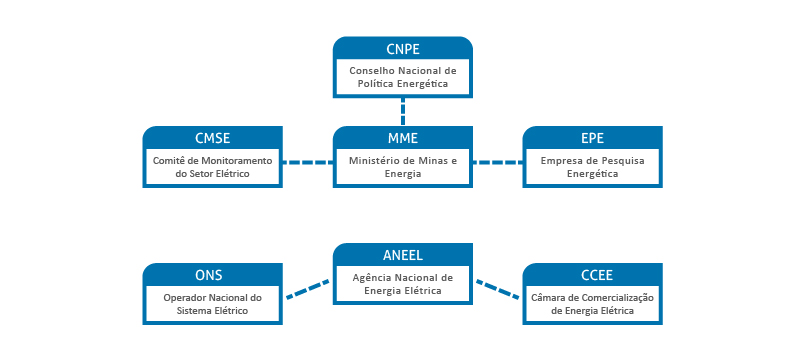
\includegraphics[width=1\linewidth]{orgaos_governo.jpg}
		\caption[\small{Institui��es do setor el�trico brasileiro \cite{}.}]{\label{instituicoesSEB} \small{Institui��es do setor el�trico brasileiro. Fonte: EPE \cite{CCEE}.}}
	\end{figure}
\end{itemize} 


\paragraph{}Outra medida tomada para facilitar o gerenciamento de toda a rede de gera��o, transmiss�o, e consumo de energia el�trica foi dividir o Sistema Interligado Nacional - SIN\cite{ONS} em quatro subsistemas sendo estes: Norte, Nordeste, Sudeste/Centro-Oeste e Sul. Vale ressaltar que existe conex�o entre as partes, de forma que um subsistema pode auxiliar o suprimento da demanda de energia de outro em per�odos de seca. Participam desse sistema diversos agentes\cite{CCEE}, sendo eles: 

\begin{itemize}
	\item{\textbf{Agentes geradores}: s�o agentes autorizados a gerar energia el�trica para o sistema.}
	
	\item{\textbf{Agentes de transmiss�o}: s�o agentes que detem o meios de transmiss�o de energia.}
	
	\item{\textbf{Agentes de distribui��o}: s�o agentes autorizados a distribuir energia contratada dos servi�os de transmiss�o em uma �rea definida pela concess�o}
	
	\item{\textbf{Consumidores livres}: s�o consumidores que tem a op��o de escolher o distribuidor de energia, diferente do que acontece no consumo dom�stico.}
	
	\item{\textbf{Agentes importadores}: s�o agentes titulares de autoriza��o expedida pela ANEEL para exercer as atividades de importa��o de energia el�trica.}
	
	\item{\textbf{Agentes exportadores}: s�o agentes titulares de autoriza��o para implanta��o de sistemas de transmiss�o associados � exporta��o de energia el�trica.}
	
	\item{\textbf{Agente comercializador da energia de Itaipu}: por ser uma usina binacional, segue tratos espec�ficos. Atualmente a comercializa��o desta energia � coordenada pela Eletrobras.}
\end{itemize}

\begin{figure}[H]
	\begin{center}
		
		\parbox[htb]{13.0cm}
		
		{
			
			\begin{center}
				
				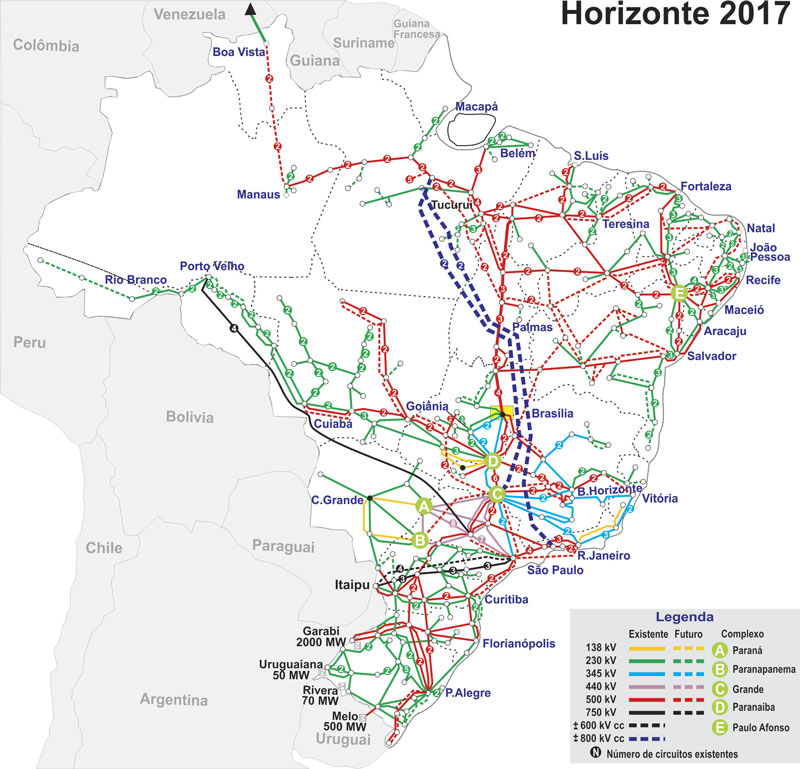
\includegraphics[scale=0.6]{SistemadeTransmissao_Horizonte2017.jpg}
				
				\caption[\small{Mapa do Sistema El�trico Brasileiro no horizonte de 2017 \cite{ONS} }]{\label{MapaH2017} \small{Mapa do Sistema El�trico Brasileiro no horizonte de 2017\cite{ONS}}}
				
			\end{center}
			
		}
		
	\end{center}
	
\end{figure}

\paragraph{}A reestrutura��o tamb�m dividiu o mercado de energia el�trica brasileiro em dois ambientes de comercializa��o: Ambiente de Contrata��o Regulada - ACR e Ambiente de Contrata��o Livre - ACL. O primeiro ambiente � focado na contrata��o de energia para consumidores residenciais e ind�strias de baixo consumo em geral. As negocia��es s�o feitas atrav�s de leil�es onde geralmente os contratos de fornecimento de energia tem foco no m�dio e longo prazo (dura��o maior que 5 anos). As distribuidoras s�o obrigadas a comprar 100\% da energia utilizada atrav�s desse meio. O segundo ambiente � focado em contrata��es bilaterais, de forma a trazer benef�cios para grande consumidores, conforme mostrado abaixo, pois podem negociar o pre�o da energia direto com os geradores \cite{PRECO_SPOT}. Os agentes que podem realizar compra por esse tipo de mercado s�o os agentes livres, conforme mostrados na tabela a seguir:

\begin{table}[h]
	
	\begin{center}
		
		\caption{Crit�rios vigentes para se tornar consumidor Livre \cite{CCEE}.}
		
		\begin{tabular}{|c|c|c|}\hline
			
			\textbf{Demanda M�nima} & \textbf{Tens�o m�nima de fornecimento} & \textbf{\makecell{Data da liga��o \\do consumidor}}\\ \hline \vspace{-1.0mm}
			
			3MW & Qualquer Tens�o & Ap�s 07/07/1995 \\ \hline 
			3MW & 69KV & Ap�s 07/07/1995 \\ \hline
		\end{tabular}
		
	\end{center} 
	\label{table:RegrasConsumidorLivre}
	
\end{table}

\paragraph{} Dado o dinamismo do consumo, dificilmente a energia utilizada ser� igual a contratada. Uma das fun��es da CCEE � realizar medi��es tanto do que � produzido quanto o que � consumido. Esta institui��o concentra informa��es sobre o montante de energia negociado em cada contrato do SEB. A diferen�a entre o que foi negociado e o que foi consumido  � liquidado utilizando como multiplicador o Pre�o de Liquida��o das Diferen�a - PLD, o qual ser� explicado mais a frente. O saldo dos agentes no mercado de curto prazo se d� pelas seguintes equa��es\cite{PRECO_SPOT}. 

\begin{equation} \label{ReceitaGerador}
	Receita_{Gerador} = (Energia_{Gerada} - Energia_{Contratada})  * PLD
\end{equation}
\begin{equation} \label{ReceitaConsumidor}
	Despesa_{Consumidor} = (Energia_{Consumida} - Energia_{Contratada})  * PLD
\end{equation}

\paragraph{}Esse processo de liquida��o das diferen�as � realizado entre as partes envolvidas na negocia��o. A CCEE somente realiza o c�lculo de quanto cada contraparte deve pagar ou receber. A import�ncia do PLD n�o se resume somente ao MCP, pois muitos dos contratos do mercado livre s�o baseados nesse valor\cite{PrevisaoPrecoFuturoACL}. Isto permite que os agentes tomem estrat�gias diferentes para aumentar o lucro ou diminuir o preju�zo. Um exemplo disso seria um agente consumidor, que ao prever o aumento de pre�os nos pr�ximos meses, pode buscar realizar contratos para abastecimento futuro a um pre�o menor do que seria pago. Outro exemplo seria um distribuidor, que ao prever um baixo PLD no MCP do m�s atual, decide vender o excedente de energia contratada no mercado livre ao inv�s de receber o valor proporcional ao PLD.

\section{O C�lculo do Pre�o da Liquida��o das Diferen�as}
O grande desafio do setor � utilizar a energia de maneira eficiente, reduzindo o custo da mesma e o risco de deficit tanto no m�s atual quanto nos meses seguintes. Isto demanda a cria��o e utiliza��o de novas tecnologias auxiliares ao planejamento.

\paragraph{}Conforme observado na figura abaixo, o pre�o depende diretamente da quantidade de �gua nos reservat�rios e a previs�o de quanto �gua estar� armazenada nos meses futuros.

\begin{figure}[H]
	\begin{center}
		{
			\begin{center}
				
				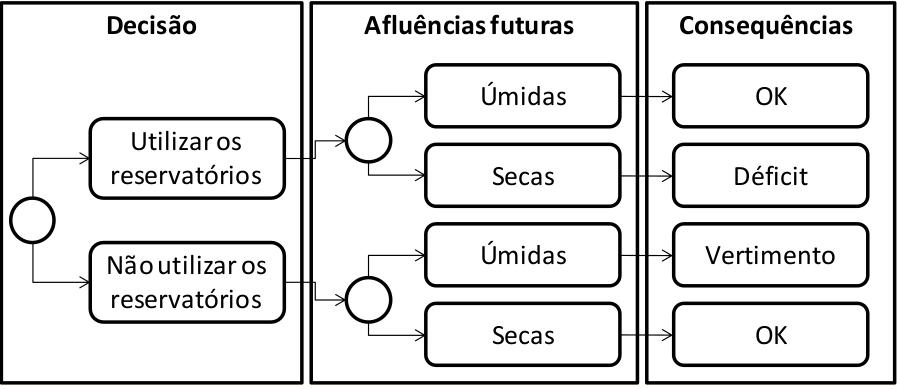
\includegraphics[scale=0.475]{decisao.jpg}
				
				\caption[\small{Mapa do Sistema El�trico Brasileiro no horizonte de 2017 \cite{PrevisaoMultiPassos} }]{\label{Decisao} \small{Planejamento da produ��o de energia do sistema hidrot�rmico\cite{PrevisaoMultiPassos}}}
				
			\end{center}
			
		}
		
	\end{center}
	
\end{figure}

\paragraph{}Sendo assim, utilizar as usinas hidrel�tricas - UHEs na capacidade m�xima gerar� o menor custo de energia poss�vel no m�s atual, por�m, se no futuro for necess�rio utilizar outras fontes para suprir a demanda energ�tica, o custo pode ser muito maior do que em uma situa��o onde a produ��o energ�tica da UHE foi distribu�da durantes os meses consecutivos. Por um outro lado, caso a a quantidade de �gua armazenada em um reservat�rio supere o limiar m�ximo do mesmo, torna-se necess�rio liberar o excedente para o rio, situa��o chamada de "vertimento". Isto � indesej�vel, pois resulta em um desperd�cio de energia barata. Portanto, um planejamento equivocado pode causar altas no PLD, o que afeta diretamente os agentes que participam do mercado de energia el�trico brasileiro.


\paragraph{}O Brasil atualmente possui uma matriz el�trica diferente do que em geral � observado no mundo. Em m�dia 65,2\% da energia utilizada no pa�s vem de fontes hidr�ulicas, diferente do que ocorre em m�dia no resto do mundo (aproximadamente 16,6\%), assim como visto em\cite{EPE}. Essa fonte al�m de ser renov�vel, tem impacto menor no meio ambiente e custos menores quando comparado com fontes baseadas em combust�veis f�sseis. O grande ponto negativo � a caracter�stica vol�til desse recurso, pois depende baste de condi��es clim�ticas, o que dificulta o planejamento para per�odos longos.

\begin{figure}[H]
	\centering
	\begin{subfigure}{.47\textwidth}
		\centering
		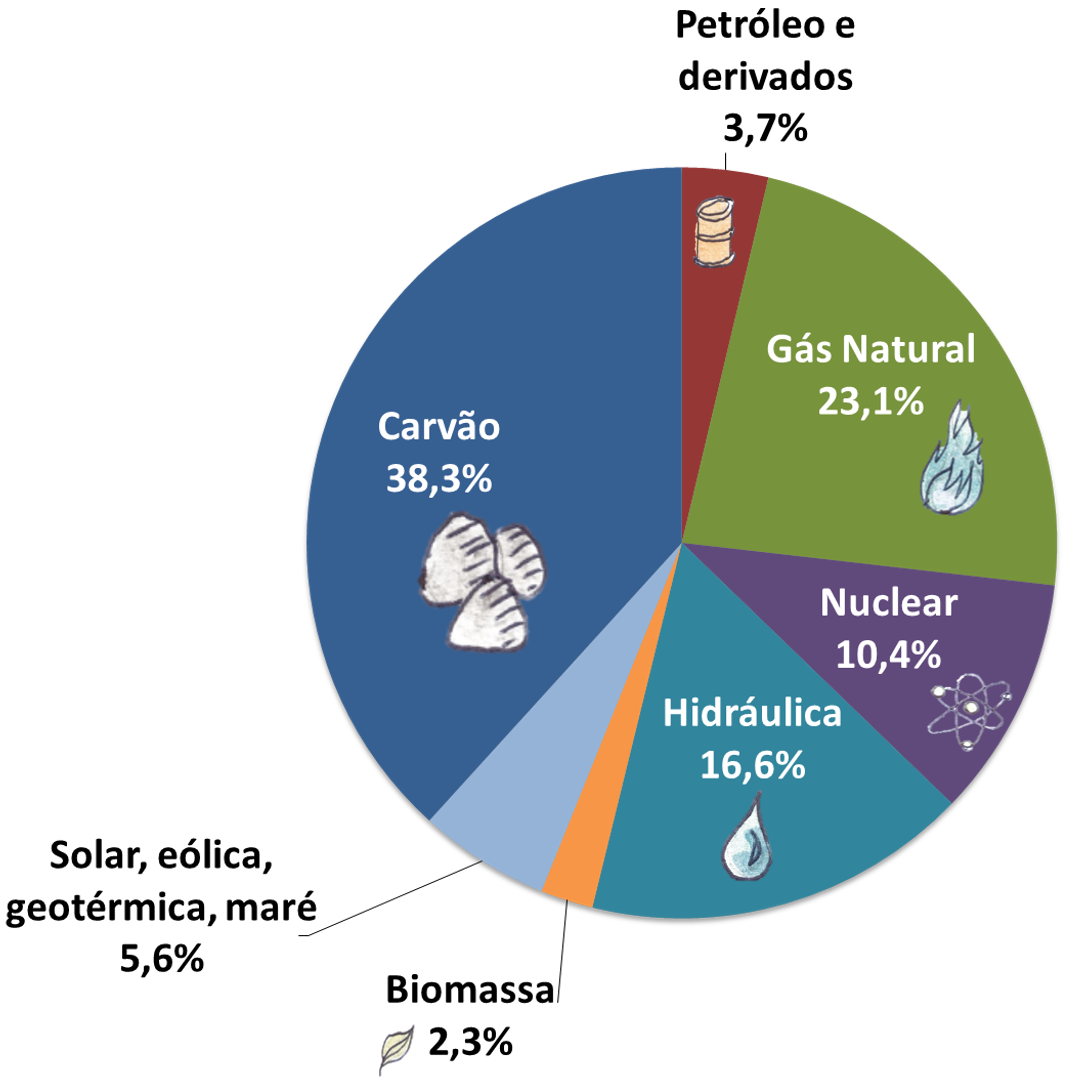
\includegraphics[width=1\linewidth]{matrizEletrica_mundo.png}
		\caption[\small{Matriz El�trica Mundial \cite{EPE}.}]{\label{matrizEletricaMundial} \small{Matriz El�trica Mundial. Fonte: EPE \cite{EPE}.}}
		
	\end{subfigure}\hfill
	\begin{subfigure}{.48\textwidth}
		\centering
		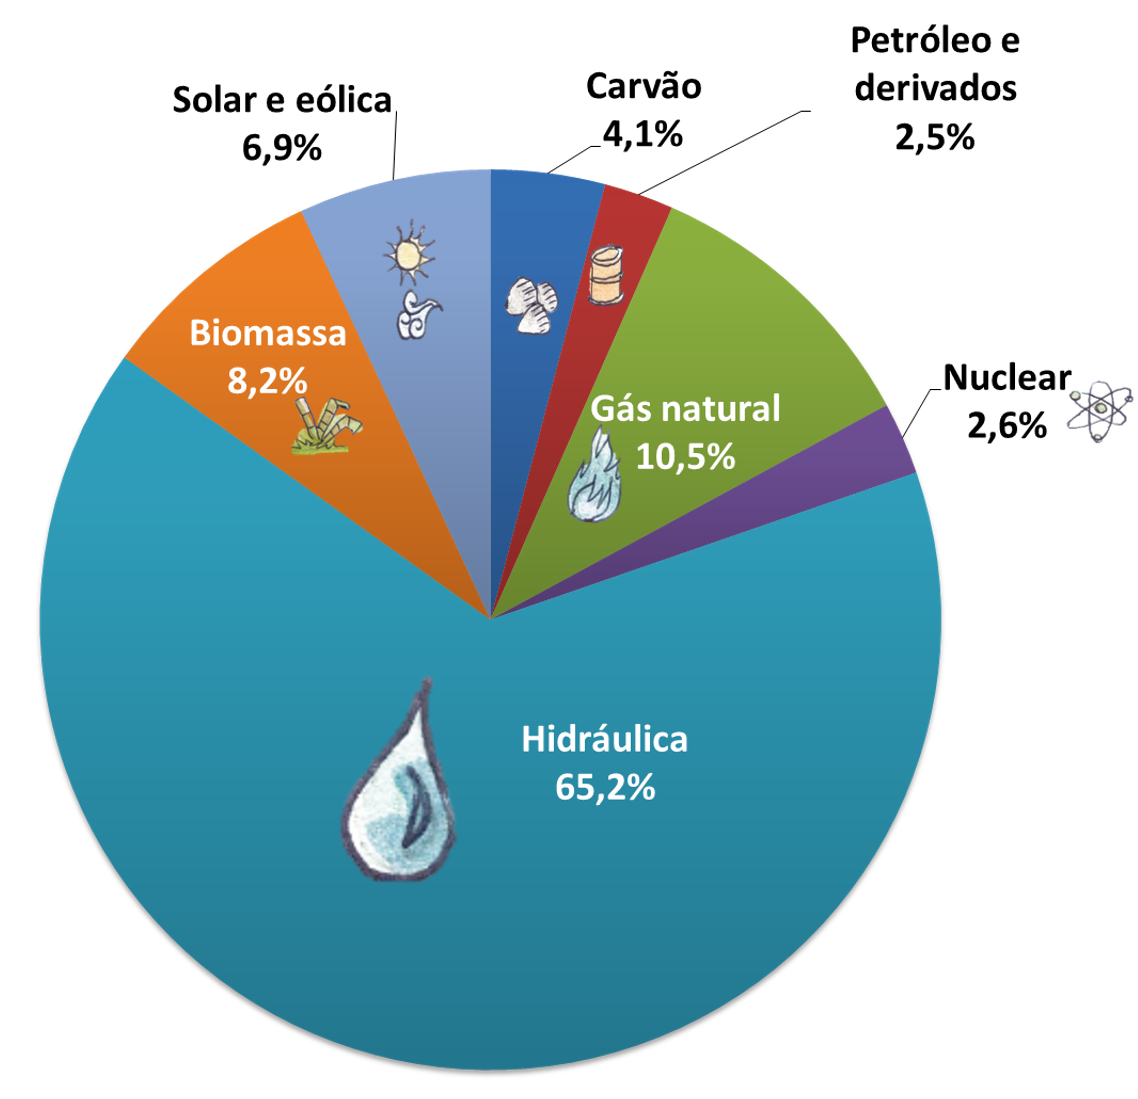
\includegraphics[width=1\linewidth]{matrizEletrica_brasil.png}
		\caption[\small{Matriz El�trica Mundial \cite{EPE}.}]{\label{matrizEletricaBrasil} \small{Matriz El�trica Brasileira. Fonte: EPE \cite{EPE}.}}
	\end{subfigure}
	\caption{Compara��o entre a matriz el�trica mundial e a brasileira}
	\label{fig:MatrizEletricaComparacao}
\end{figure}

\paragraph{}Uma tend�ncia mundial no setor � a transi��o da rede el�trica atual para o smart grid. Este termo engloba uma s�rie de tecnologias, tendo como foco o sensoriamento dos componentes que comp�em a rede. Isto permite ter informa��es sobre o consumo em um per�odo de tempo menor do que nas redes antigas, al�m de conseguir averiguar falhas na rede de maneira remota, mudando a postura das distribuidoras de reativa para ativa, pois torna-se poss�vel resolver os erros antes que os clientes liguem para a concession�ria.

\paragraph{}Assim como visto em \cite{SmartGrid}, no ano de 2012 a ANEEL aprovou a resolu��o normativa No 482 \cite{RES_NORMA_482}, que "Estabelece as condi��es gerais para o acesso de microgera��o e minigera��o distribu�da aos sistemas de distribui��o de energia el�trica, o sistema de compensa��o de energia el�trica, e d� outras provid�ncias". Desde mar�o de 2016 � permitido que qualquer fonte de energia renov�vel participe do sistema de gera��o distribu�do, n�o limitando somente � solar e � e�lica. Sendo assim a tend�ncia � que parte da produ��o de energia seja proveniente de pequenos geradores, diminuindo parcialmente a depend�ncia de grandes produtores de energia, o que pode acarretar na redu��o do risco de deficit de energia.

\begin{figure}[H]
	\centering
	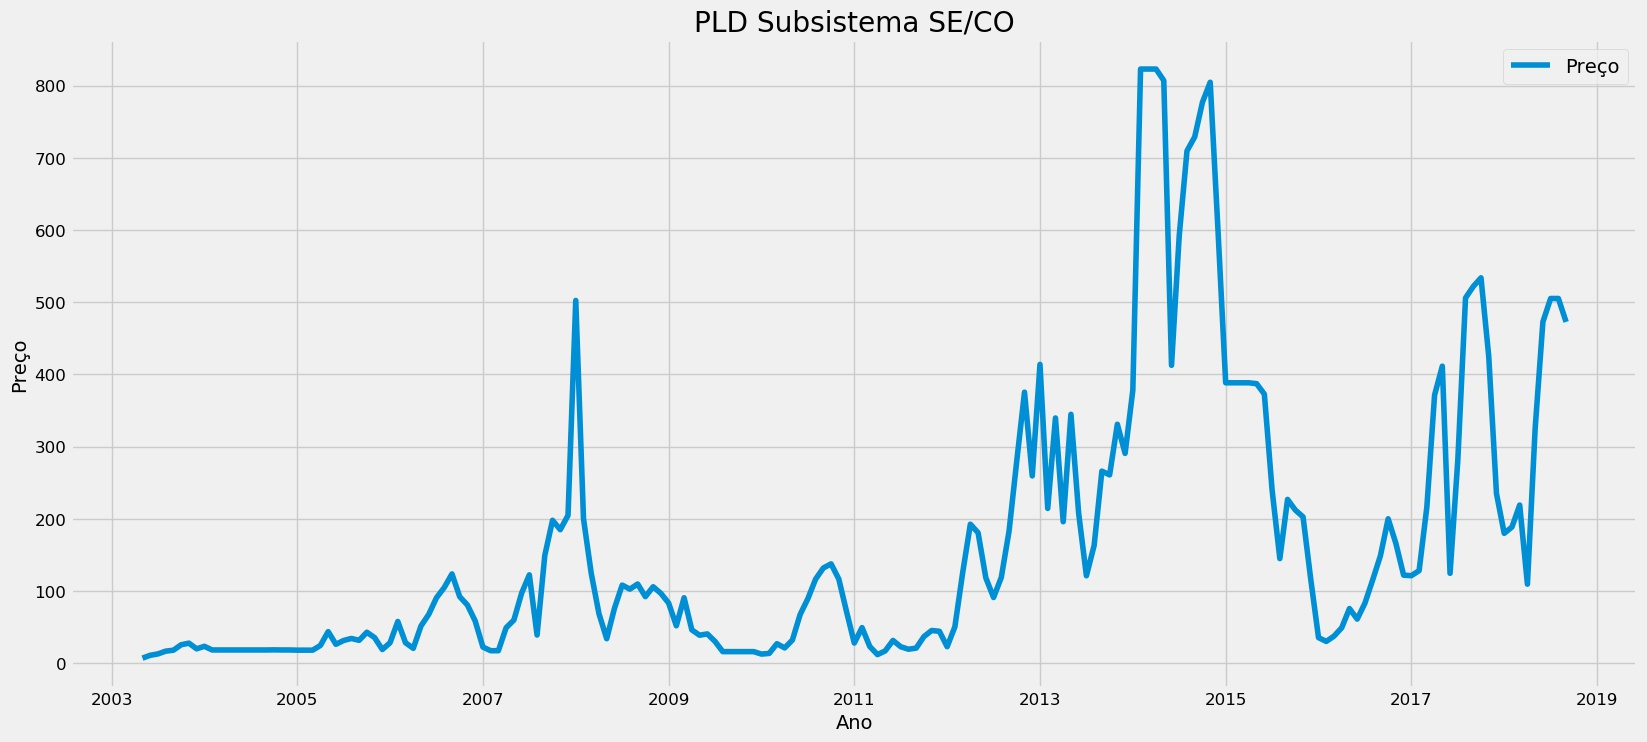
\includegraphics[width=1\linewidth]{PLD_media_mensal_SE.jpg}
	\caption[\small{Institui��es do setor el�trico brasileiro \cite{CCEE}.}]{\label{PLDMensal} \small{Institui��es do setor el�trico brasileiro. Fonte: CCEE \cite{CCEE}.}}
\end{figure}

\paragraph{}No gr�fico acima observa-se que existem pontos onde o SIN foi afetado por crises, fazendo com que o PLD aumentasse abruptamente. No ano de 2007 ocorreu a primeira mostrada no gr�fico. O SEB tinha passado por uma recente reestrutura��o da organiza��o, a qual n�o foi suficiente para evitar o acontecimento. Durante o per�odo de racionamento (2001/06 - 2002/02) a demanda foi menor do que a oferta, por�m com o passar do anos ela voltou a se aproximar da curva de oferta. Ap�s abril de 2005, houve um per�odo sem investimento na capacidade energ�tica sistema. Junto com esse fato, ocorreu um per�odo de baixa aflu�ncia nas usinas hidrel�tricas.

\paragraph{}Outra crise not�vel ocorreu no ano de 2014, onde segundo \cite{CRISE_2014}, houve a diminui��o das tarifas imposta pelo governo em um momento de demanda crescente, o atraso em obras de gera��o e transmiss�o, al�m da escassez de chuvas.

\paragraph{}O PLD � calculado semanalmente e disponibilizado sexta-feira pela CCEE conforme a f�rmula \ref{FormulaPrecoPLD}, com vig�ncia na semana seguinte. Para cada um dos submercados do SIN s�o divulgados valores para os tr�s patamares de carga: leve, m�dio e pesado. Esses est�o relacionados com a hora do dia e o consumo, sendo que o patamar � pesado em hor�rios de alto consumo e leve nos per�odo de baixo demanda energ�tica. O PLD mensal por subsistema � calculado tamb�m pela CCEE atrav�s da m�dia dos pre�os ponderadas pelo tempo em cada patamar.

\begin{equation} \label{FormulaPrecoPLD}
PLD_{s, r, \omega} = min(max(CMO_{s, r, \omega}, PLD_{min_{ano}}), PLD_{max_{ano}})
\end{equation}

\paragraph{} Onde:
\begin{table}[h]

	\begin{center}

		\caption{Vari�veis utilizadas no c�lculo do PLD semanal \cite{CCEE}.}

		\begin{tabular}{|c|c|}\hline

			\textbf{Vari�vel} & \textbf{Significado}\\ \hline \vspace{-1.0mm}

			$s$ & Subsitema ("N", "NE", "S", "SE\textbackslash CO") \\ \hline \vspace{-1.0mm}
			$r$ & Patamar de carga ("leve", "m�dio", "pesado")
\\ \hline \vspace{-1.0mm}
			$w$ & Semana do m�s \\ \hline \vspace{-1.0mm}
			CMO & Custo para produ��o de um MWh adicional no SIN \\ \hline \vspace{-1.0mm}
			$PLD_{min_{ano}}$ & PLD m�nimo estabelecido anualmente pela ONS \\ \hline
			$PLD_{max_{ano}}$ & PLD m�ximo estabelecido anualmente pela ONS \\ \hline
		\end{tabular}

	\end{center} 
	\label{table:VariaveisPLD}

\end{table}

\paragraph{}O PLD m�ximo � calculado com base no custo vari�vel unit�rio - CVU mais elevado de uma Usina t�rmica - UTE em opera��o comercial, a g�s natural, contratada por meio Contrato de Comercializa��o de Energia El�trica no Ambiente Regulado - CCEAR , definido no planejamento mensal de opera��o - PMO de dezembro e ser� aplicado entre a primeira e �ltima semana operativa do ano subsequente, para todos os submercados.

\paragraph{}O PLD m�nimo � calculado com base no maior valor entre: i) o calculado com base na Receita Anual de Gera��o- RAG  das usinas hidrel�tricas em regime de cotas, nos termos da Lei n� 12.783/2013, exclu�dos os valores relacionados � remunera��o e reintegra��o de investimentos, e adicionada a estimativa de Compensa��o Financeira pelo Uso dos Recursos H�dricos - CFURH; e ii) as estimativas dos custos de gera��o da usina de Itaipu para o ano seguinte, fornecidas pela Itaipu Binacional para fins de reajustes e/ou revis�es tarif�rias.

O valores de definidos para os �ltimos 5 anos foram:
\begin{table}[H]
	
	\begin{center}
		
		\caption{Pre�o m�nimo e m�ximo do PLD \cite{CCEE}.}
		
		\begin{tabular}{|c|c|c|}\hline
			
			\textbf{Ano} & \textbf{PLD M�nimo} & \textbf{PLD M�ximo}\\ \hline \vspace{-1.0mm}
			
			2015 & 30,26 & 388,48 \\ \hline \vspace{-1.0mm}
			2016 & 30,25 & 422,56  \\ \hline \vspace{-1.0mm}
			2017 & 33.68 & 533.82 \\ \hline \vspace{-1.0mm}
			2018 & 40,16 & 505,18 \\ \hline
			2019 & 42,35 & 513,89 \\ \hline 
		\end{tabular}
		
	\end{center} 
	\label{table:PLD_MIN_MAX}
	
\end{table}


\paragraph{}O planejamento e o c�lculo do PLD � feito com base em programas desenvolvidos especificamente para o SIN. 
Algum deles s�o \cite{MANUAIS}:
\begin{itemize}
	\item{NEWAVE: Utilizado no planejamento de m�dio prazo (at� 5 anos), com espa�amento mensal entre as previs�es}
	\item{DECOMP: Utilizado no planejamento de curto prazo (at� 12) com base semanal}
\end{itemize}
c�lculo do PLD � feito com base no CMO obtido do programa DECOMP, o qual � disponibilizado somente para agentes cadastrados no CCEE e tem como entrada os seguintes dados:

\begin{table}[H]
	
	\begin{center}
		
		\caption{Arquivos de entrada do DECOMP \cite{CCEE}.}
		
		\begin{tabular}{|c|c|}\hline
			
			\textbf{Arquivo} & \textbf{Conte�do}\\ \hline \vspace{-1.0mm}
			
			CASO.DAT & Cont�m o nome do Arquivo �ndice\\ \hline \vspace{-1.0mm}
			Arquivo �ndice & \makecell{Cont�m a lista de arquivos de entrada \\ sob gerenciamento do usu�rio}\\ \hline \vspace{-1.0mm}
			DADGER.DAT & Dados gerais de planejamento\\ \hline \vspace{-1.0mm}
			VAZOES.XXX & \makecell{Vaz�es incrementais afluentes aos aproveitamentos da \\ configura��o considerada}\\ \hline \vspace{-1.0mm}
			HIDR.DAT & Cadastros de dados das usinas\\ \hline \vspace{-1.0mm}
			MLT.DAT & M�dias mensais de longo termo\\ \hline \vspace{-1.0mm}
			LOSS.DAT & Perdas no sistema\\ \hline
			DADGNL.XXX & dados de usinas t�rmicas\\ \hline
		\end{tabular}
		
	\end{center} 
	\label{ArquivosEntradaDECOMP}
	
\end{table}
\paragraph{}O Termo MLT - M�dia de Longo Termo se refere � m�dia com per�odo anual, utilizando uma s�rie hist�rica dos valores de ENA - Energia Natural Afluente para cada um dos meses desde 1931. A ENA, por sua vez � a energia que pode ser gerada atrav�s a partir da vaz�o da �gua em uma determinada bacia.

\paragraph{}O arquivo HIDR.DAT, MLT.DAT e VAZOES.DAT vem em formato bin�rio e para serem lidos pelo operador, precisam de programas auxiliares para a convers�o, sendo eles Hydroedit para o primeiro e Vazedit para os dois �ltimos. Ambos s�o fornecidos pela ONS. J� arquivo de dados gerais tem 43 par�metros, sendo alguns deles contratos de importa��es/exporta��o de energia, custo de d�ficit e a fun��o de custo futuro. Esta �ltima determinada pelo NEWAVE.

\paragraph{}Obter um modelo matem�tico baseado no DECOMP que possa ser utilizado na previs�o do PLD � de interesse n�o s� dos agentes que participam do mercado el�trico brasileiro, como tamb�m de empresas indiretamente relacionadas ao setor como consultorias e bancos, al�m de existir o vi�s acad�mico, pois o entendimento da din�mica do pre�o pode ajudar na formula��o de novos modelo de previs�o e altera��o do j� existente, buscando melhoras nas atividades de planejamento feitas pelos �rg�os.

\section{Revis�o bibliogr�fica}
\paragraph{}Em \cite{TCC_PLD} foi utilizada uma abordagem onde s�o previstos os valores de energia afluente, energia proveniente de hidroel�tricas, energia proveniente de usinas t�rmicas e carga dos subsistemas, a fim de obter o valor do PLD indiretamente. A outra forma proposta foi utilizar a pr�pria informa��o sobre o PLD na previs�o do mesmo. Em ambos os casos, foram utilizadas redes neurais artificiais autorregressiva n�o-linear - NARNET e os valores previstos s�o para at� 3 semanas � frente.

\begin{figure}[H]
	\centering
	\begin{subfigure}{.47\textwidth}
		\centering
		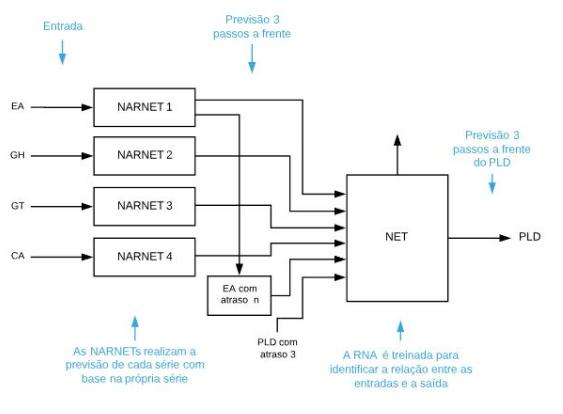
\includegraphics[width=1\linewidth]{esquematico_previsao_indireta_pld_ufop_tcc.jpg}
		\caption[\small{Esquematico previs�o indireta do PLD \cite{TCC_PLD}.}]
		{\label{EsquematicoPrevisaoIndiretaPLDUFOP} \small{Esquematico previs�o indireta PLD\cite{TCC_PLD}.}}
		
	\end{subfigure}\hfill
	\begin{subfigure}{.48\textwidth}
		\centering
		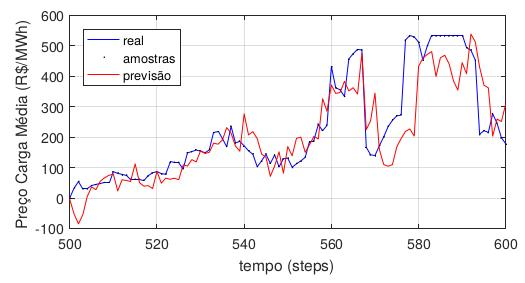
\includegraphics[width=1\linewidth]{previsao_indireta_pld_ufop_tcc.jpg}
		\caption[\small{Previs�o indireta do PLD \cite{TCC_PLD}.}]
		{\label{PrevisaoIndiretaPLDUFOP} \small{Previs�o indireta do PLD \cite{TCC_PLD}.}}	
	\end{subfigure}\hfill
	\caption{Previs�o indireta do PLD}
	\label{fig:PrevisaoIndiretaPLDUFOP}
\end{figure}

\begin{figure}[H]
	\centering
	\begin{subfigure}{.47\textwidth}
		\centering
		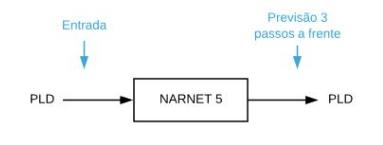
\includegraphics[width=1\linewidth]{esquematico_previsao_direta_pld_ufop_tcc.jpg}
		\caption[\small{Esquematico previs�o indireta do PLD \cite{TCC_PLD}.}]
		{\label{EsquematicoPrevisaoDiretaPLDUFOP} \small{Esquematico previs�o direta do PLD\cite{TCC_PLD}.}}
	\end{subfigure}
	\begin{subfigure}{.47\textwidth}
		\centering
		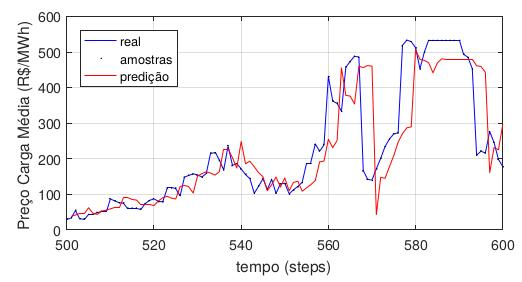
\includegraphics[width=1\linewidth]{previsao_direta_pld_ufop_tcc.jpg}
		\caption[\small{Previs�o direta do PLD \cite{}.}]
{\label{PrevisaoDiretaPLDUFOP} \small{Previs�o direta PLD\cite{TCC_PLD}.}}
	\end{subfigure}
	\caption{Previs�o direta do PLD}
	\label{fig:PrevisaoDiretaPLDUFOP}	
\end{figure}

\paragraph{}Outras abordagens s�o vistas em \cite{PrevisaoMultiPassos}, onde � proposto um modelo h�brido com a utiliza��o de modelo autorregressivo de m�dia m�vel integrada sazonal - SARIMA, an�lise de componentes principais e redes neurais, conforme a figura a seguir:

\begin{figure}[H]
	\centering
	\begin{subfigure}{.47\textwidth}
		\centering
		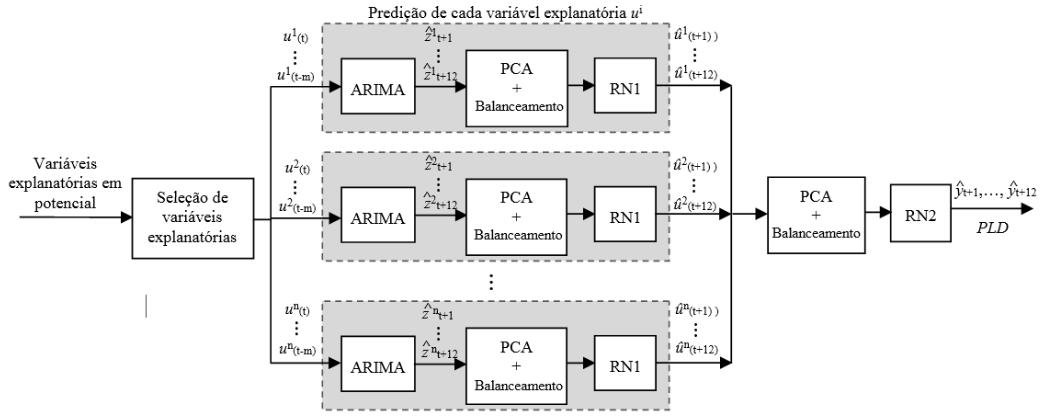
\includegraphics[width=1\linewidth]{hibrido_tese_PLD.jpg}
		\caption[\small{Esquematico previs�o indireta do PLD \cite{PrevisaoMultiPassos}.}]
		{\label{HibridoTesePLD} \small{Esquematico modelo h�bdrido de previs�o do PLD. \cite{PrevisaoMultiPassos}.}}
	\end{subfigure}
	\begin{subfigure}{.4659\textwidth}
		\centering
		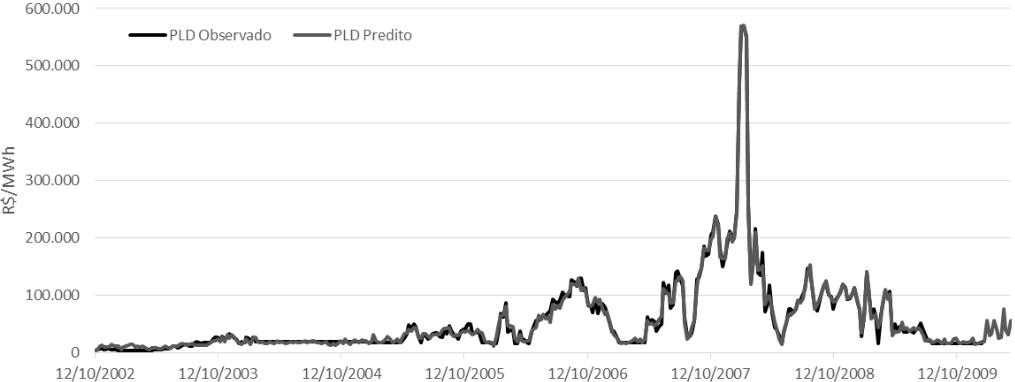
\includegraphics[width=1\linewidth]{resultado_tese_previsao_PLD_se_co.jpg}
		\caption[\small{Resultado da previs�o do modelo h�brido \cite{PrevisaoMultiPassos}.}]
		{\label{ResultadoHibridoTesePLD} \small{Resultado da previs�o do modelo h�brido. \cite{PrevisaoMultiPassos}.}}
	\end{subfigure}
	\caption{Previs�o do PLD utilizando o modelo h�brido}
	\label{fig:ResultadoPrevisaoMultiPassos}		
\end{figure}

\paragraph{}Na segunda abordagem proposta pelo mesmo autor utilizou-se uma combina��o do algoritmo C5.0 e �rvore de classifica��o e regress�o - CART para determinar se o pre�o do PLD ser� estar� dentro de um patamar num instante futuro.

\begin{figure}[H]
	\centering
	\begin{subfigure}{.5\textwidth}
		\centering
		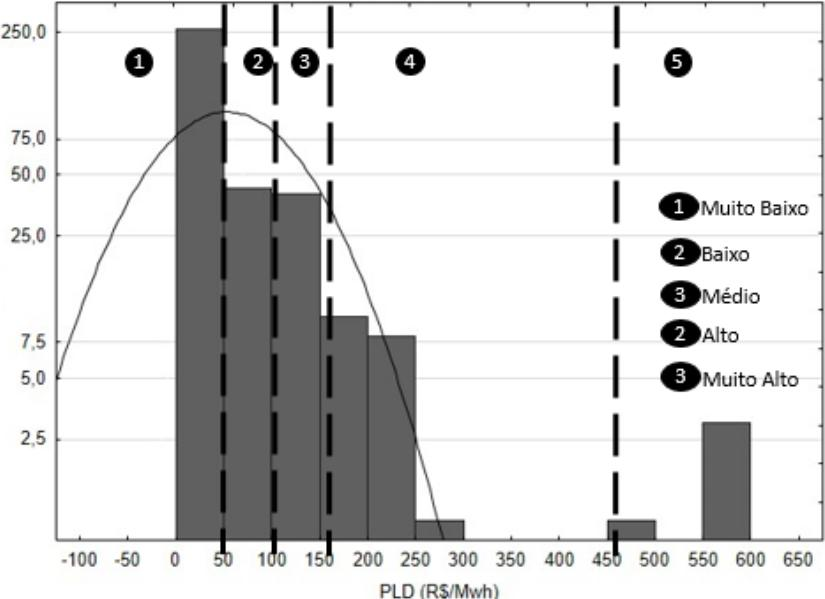
\includegraphics[width=1\linewidth]{divisoes_previsao_tese.jpg}
		\caption[\small{Classes de sa�da do algor�tmo\cite{PrevisaoMultiPassos}.}]
		{\label{ClassesPrevisao} \small{Classes de sa�da do algor�tmo \cite{PrevisaoMultiPassos}.}}
	\end{subfigure}
	\begin{subfigure}{.6\textheight}
		\centering
		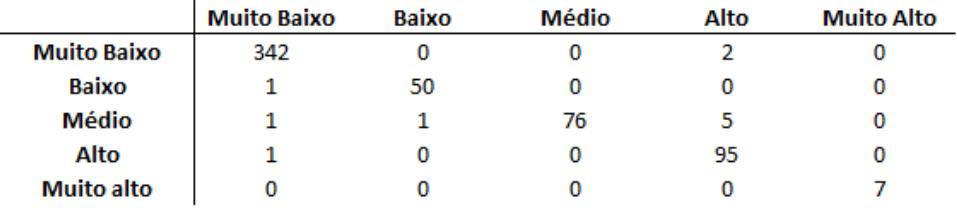
\includegraphics[width=1\linewidth]{resultado_classificador_tese_previsao.jpg}
		\caption[\small{Matriz de confus�o \cite{PrevisaoMultiPassos}.}]
		{\label{ResultadoClassificadorTesePLD} \small{Matriz de confus�o \cite{PrevisaoMultiPassos}.}}
	\end{subfigure}
	\caption{Previs�o do PLD utilizando o modelo h�brido}
	\label{fig:ResultadoPrevisaoMultiPassosClassificador}		
\end{figure}

\paragraph{}Em ambos o casos acima o autor realiza previs�es para um per�odo de 12 semanas � frente.

\paragraph{}No trabalho visto em \cite{RNA_DIRETA_E_RECORRENTE}, , t�m se a an�lise das vari�veis utilizadas na entrada de cada submercado atrav�s da correla��o. Al�m � feita a compara��o entre os resultados obtidos pelo modelo ARIMA, rede neura recorrente, rede neural direta sem sele��o de lags e com a sele��o de lags. J� em \cite{RNA_PRECO_SPOT} foram utilizadas como vari�veis de entrada a gera��o das hidroel�tricas, t�rmicas e e�lica, al�m da Energia Natural Afluente - ENA, ENA m�xima, EAR - Energia Armazenada e o PLD para cada um dos patamares nas 4 �ltimas semanas, utilizando uma rede neural com 3 neur�nios na camada interna. Com m�trica utilizada, faz-se um plot do alvo pelo resultado previsto pela rede e ent�o � feito uma ajuste linear. No caso ideal a equa��o $y = a\cdot x + b$ se torna $y = x$ (previs�o perfeita) para a previs�o em um horizonte de at� 6 semanas. Em \cite{TCC_FABIANE} utiliza-se uma rede neural recorrente para obter previs�es em um horizonte de at� seis meses a frente.

\paragraph{}Outra abordagem diferente das observadas acima � a vista em \cite{GARCH_PLD}, onde o autor utiliza modelos \textit{Genralized Auto-Regressive Conditional Heteroscedasticity}- GARCH para a previs�o do PLD. Para a estima��o dos par�metros foram utilizadas an�lises com base na fun�ao de autocorre��es - ACF, autocorrela��es parciais - PACF, fun��o de verossimilhan�a (LLF) e testes estat�sticos como o \textit{Akaike info criterion} - AIC.

\paragraph{}A previs�o do pre�o da energia el�trica � um interesse comum de v�rios agentes envolvidos com o mercado de energia mundialmente. Em \cite{PSF_forecast} o autor utiliza o algoritmo \textit{K-means} para clusterizar os dados de entrada passados e o algoritmo \textit{Partial Sequence-based Forecasting} - PSF para prever o resultado com base na m�dia dos resultados obtidos no clusters anteriores. O modelo obtido foi utilizado para prever pre�o e demanda de energia para o mercado espanhol, australiano e nova-iorquino e obteve resultados relevantes.

\begin{figure}[H]
	\centering
	\includegraphics[width=1\linewidth]{PSF_forecast.jpg}
	\caption[\small{Institui��es do setor el�trico brasileiro \cite{PSF_forecast}.}]{\label{PSF_forecast} \small{Utiliza��o do algoritmo PSF para previs�o de s�ries temporais \cite{PSF_forecast}.}}
\end{figure}

\paragraph{}Em \cite{simple_forecast} s�o mostradas algumas abordagem simples para o problema de previs�o do pre�o \textit{spot} (PLD � um exemplo de pre�o \textit{spot}) no mercado de energia de Ont�rio. Foi utilizada uma rede neural com uma camada escondida, uma rede neural misturada com l�gica fuzzy e otimiza��o com o algoritmo IMO. A previs�o foi feita hora a hora para um per�odo de 24 horas. Concluiu-se que a rede neural com l�gica fuzzy obteve o melhor resultado, al�m disso a relev�ncia das entradas para a previs�o foi analisada e viu-se que as entradas mais relevantes eram a demanda e a interrup��o do gerador. 


\paragraph{}






% ---------------------------------------------------------------
% Chapter 3 - Series Temporais e Aprendizado de M�quina
% ---------------------------------------------------------------
\chapter{Series Temporais e Aprendizado de M�quina}
\label{cap3}
\paragraph{}O objetivo deste capitulo � trazer a fundamenta��o te�rica das t�cnicas utilizadas neste trabalho. Em primeiro lugar ser� abordada a teoria, aplica��es e dificuldades relacionadas �s s�ries temporais. Logo ap�s, ser�o apresentados os modelos de aprendizados de m�quina utilizados como redes neurais MLP.

\section{S�ries Temporais}
\paragraph{}Uma s�rie temporal � composta por uma cole��o de observa��es feitas de forma sequencial e dependente \cite{sTemp}. Essa ordem da sequ�ncia � dada pelo tempo, o qual pode ser cont�nuo ou discreto. No primeiro caso, $T = {t : t_1 < t < t_2}$ e a s�rie temporal � definida como $\{X(t) : t \in T\}$, j� no segundo caso, $T = \{t_1, t_2, ... , t_n\}$ e a s�rie temporal � definida como $\{X_t : t \in T\}$, onde X � a vari�vel observada. Geralmente define-se o T para o caso discreto como $T = \{1, 2, ..., n\}$ por quest�es de simplicidade. Neste trabalho ser� utilizado o caso discreto, dado que a amostragem do sinal tem periodicidade mensal. Sendo assim, os exemplos dados no trabalho ser�o discretos tamb�m.

\paragraph{}Assim como o tempo, os valores da vari�vel $X_t$ podem ser cont�nuos ou discretos de acordo com o fen�meno que se observa. Alguns exemplos de fen�menos temporais com valores cont�nuos s�o a temperatura em um determinada regi�o, volume de �gua em uma bacia hidrogr�fica e o peso de um indiv�duo. J� como exemplo de fen�menos temporais com valores discretos podem ser citados o n�mero  viagens de avi�o, quantidade de nascimentos, de carros produzidos por uma montadora etc. Todos esse casos est�o relacionados com um per�odo de observa��o pr�prio, podendo ser uma janela de meses, anos, at� mesmo d�cadas de observa��es de uma determinada vari�vel.

\paragraph{}A an�lise de s�ries temporais pode ser feita com diferentes intuitos, sendo os mais comuns a predi��o de valores futuros com base no hist�rico j� conhecido, o controle de um processo, a explica��o e descri��o de fen�menos \cite{sTemp}.

\begin{figure}[H]
	\begin{center}
		{
			\begin{center}
				
				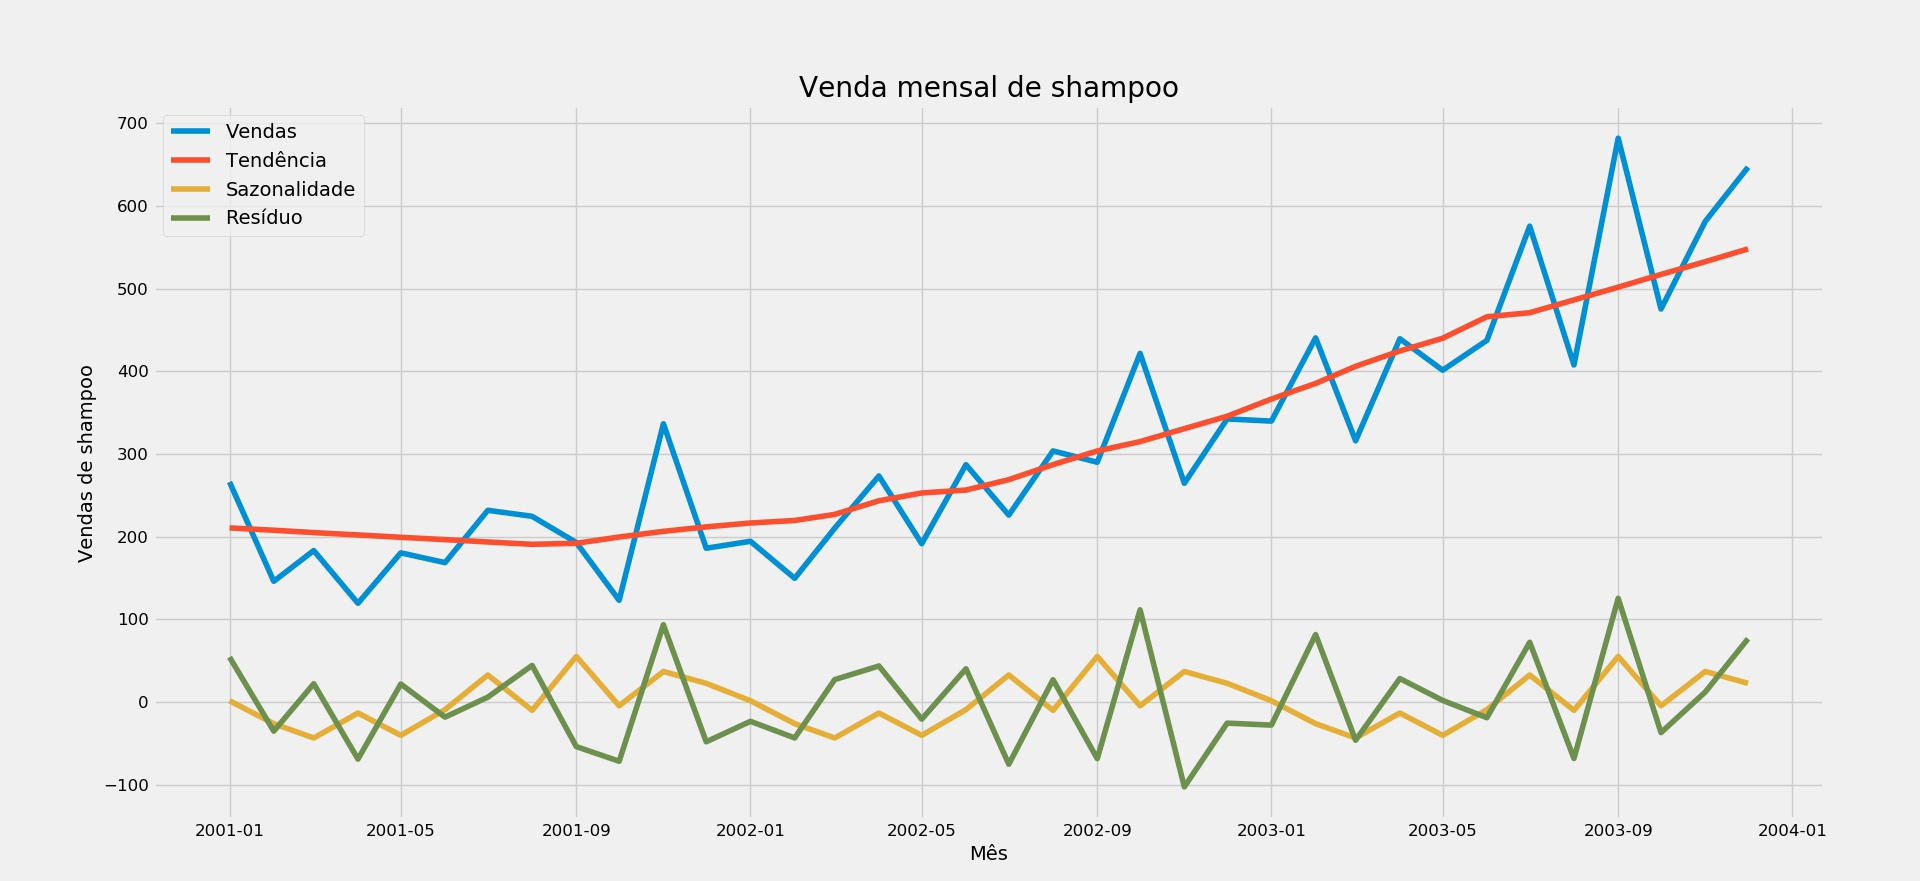
\includegraphics[width=\textwidth]{exemplo_tsa.jpg}
				
				\caption[\small{Exemplo de decomposi��o de s�rie temporal \cite{shampooSales} }]{\label{exemploTSA} \small{Exemplo de decomposi��o de s�rie temporal. Fonte:	Makridakis, Wheelwright and Hyndman (1998) \cite{shampooSales}}}
				
			\end{center}
			
		}
		
	\end{center}
	
\end{figure}

\paragraph{}Buscando tornar a an�lise das s�ries temporais mais simples, al�m de facilitar a extra��o de informa��es importantes de maneira gr�fica, � comum decompor a s�rie em outras mais simples. A decomposi��o utilizada ser� a seguinte, conforme visto em \cite{apostilaCaloba}:

\begin{equation*}
	X_t = tend_t + sz_t + cs_t + res_t
\end{equation*}

\paragraph{}Onde $tend_t$ � a tend�ncia, $sz_t$ � a sazonalidade, $cs_t$ � o ciclo senoidal e $res_t$ � o res�duo. Tanto a tend�ncia, quanto a sazonalidade e os ciclos senoidais s�o determin�sticos. Conforme \cite{tccDanilo}, boa parte das s�ries temporais s�o n�o estacion�rias, sendo que as componentes de tend�ncia e sazonalidade s�o as maiores respons�veis por esse efeito. Para que o modelo com redes neurais fa�a boas previs�es, que � o que se busca nesse trabalho, � necess�rio utilizar s�ries estacion�rias, portanto somente a parte residual ser� usada na entrada das redes neurais.

\subsection{Tend�ncia}
\paragraph{}Segundo \cite{sTemp}, a tend�ncia pode ser vista como "uma mudan�a de longo prazo no n�vel m�dio da s�rie" e a forma mais simples de modelar pode ser vista pela equa��o a seguir. 

\begin{equation}
tend_t = \alpha + \beta t + \epsilon_t
\end{equation}

\paragraph{}Onde $\alpha$ e $\beta$ s�o constantes a serem estimadas e $\epsilon_t$ denota um erro aleat�rio com m�dia zero. Geralmente chama-se o termo $m_t = \alpha + \beta t$ de termo de tend�ncia, mas alguns autores chamam o termo $\beta$ de tend�ncia, j� que $\beta = m_t - m_{t-1}$. Essa vari�vel indica a inclina��o da fun��o durante o tempo.

\paragraph{}A fun��o utilizada na aproxima��o da tend�ncia pode ser escolhida de acordo com a s�rie que est� sendo analisada. Uma forma bastante comum � a utiliza��o de uma fun��o polinomial na extra��o de tend�ncia.

\paragraph{}Na tend�ncia polinomial \ref{eqTendPoli}, busca-se fazer uma extra��o boa o suficiente para obter-se ao final do processamento a componente residual estacion�ria com m�dia zero. Para s�ries monotonicamente crescente ou decrescente, utilizar $p = 1$ (fun��o linear)  ou $p = 2$ (fun��o quadr�tica) geralmente � suficiente para a extra��o da tend�ncia, por�m caso a s�rie seja mais complexa, pode ser necess�rio utilizar fun��es de ordem mais altas

\begin{equation} \label{eqTendPoli}
tend_t = \epsilon_t + \sum_{n=0}^{p} \beta_n t^n
\end{equation}

\paragraph{}Alguns m�todos de filtragem podem ser utilizados tamb�m na extra��o de tend�ncia. � comum utilizar filtros lineares nessa tarefa. Esses s�o definidos pela seguinte equa��o:

\begin{equation}
y_t = \sum_{j = -q}^{s} a_jx_{t+j}
\end{equation}

\paragraph{}Onde $a_j$ s�o os pesos que multiplicam o sinal $x_{t+j}$. Para o filtro de m�dias m�veis geralmente utiliza-se $q=s$ e $a_{-r} = a_r$, garantindo a simetria do filtro. Al�m disso faz-se que $\sum_{j = -q}^{s} a_j = 1$, de modo que $min\{x_t\} \leq y_t \leq max\{x_t\}$. O caso mais simples de m�dia m�vel � aquele onde todos os pesos tem o mesmo valor:

\begin{equation}
y_t = \dfrac{1}{2q + 1} \sum_{j = -q}^{q} x_{t + j}
\end{equation}

\paragraph{}O resultado do filtro acima � n�o-causal, o que impede que o processamento seja utilizado para a previs�o de s�ries. Sendo assim, uma outra abordagem poss�vel � fazer um deslocamento no filtro para que sejam utilizadas somente amostras do passado, conforme a equa��o a seguir:

\begin{equation}
	y_t =  \dfrac{1}{2q + 1} \sum_{j = -2q}^{0} x_{t+j}
\end{equation} 

\paragraph{}Outro problema observado nas abordagens de m�dia m�vel descritas acima � que somente � que s� se obt�m a tend�ncia para $N - 2q$ pontos. Caso seja necess�rio obter a tend�ncia para todos os pontos da s�rie, pode-se aplicar m�todos de extrapola��o sobre o resultado obtido.

\paragraph{}Uma terceira abordagem para extra��o de tend�ncia � utilizar um filtro com pesos que decaem geometricamente, com j, priorizando assim, as amostras mais recentes da s�rie temporal:

\begin{equation}
y_t = \sum_{j=0}^{\infty} \alpha (1 - \alpha)^j x_{t-j}
\end{equation}

\begin{figure}[H]
	\begin{center}
		{
			\begin{center}
				
				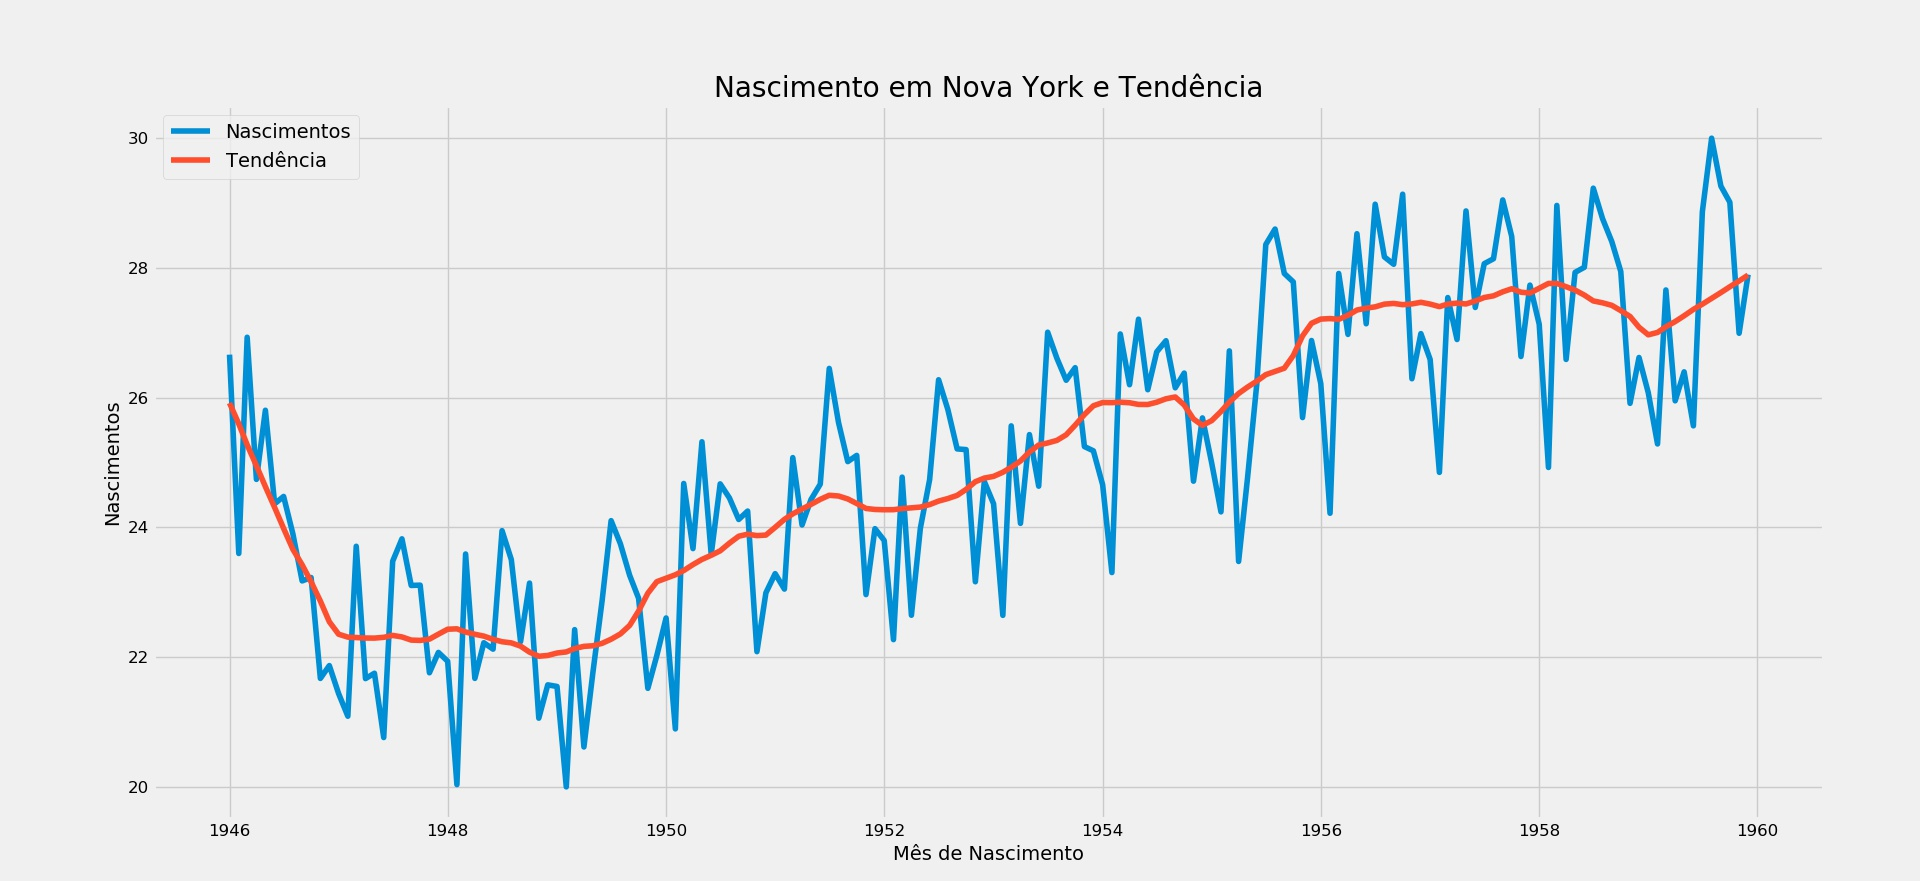
\includegraphics[width=\textwidth]{exemplo2_tendencia.jpg}
				
				\caption[\small{Exemplo de extra��o de tend�ncia com filtro de m�dia \cite{birthNY} }]{\label{bNYtend} \small{Exemplo de extra��o de tend�ncia com filtro de m�dia. Fonte: Newton (1998). \cite{birthNY}}}
				
			\end{center}	
		}
		
	\end{center}
	
\end{figure}

\paragraph{}Outra forma de extrair a tend�ncia � atrav�s da diferencia��o. Para dados n�o sazonais, a primeira diferen�a costuma ser suficiente para garantir a estacionariedade aproximada da s�rie  restante \cite{sTemp}:

\begin{equation}
y_t = x_t - x_{t-1} = \nabla x_t
\end{equation}


\subsection{Sazonalidade}
\paragraph{}� comum encontrar nas s�ries observadas alguns padr�es que se repetem periodicamente. Esse efeito � denominado sazonalidade e deve ser removido para que se obtenha ao final do processamento uma s�rie residual estacion�ria \cite{apostilaCaloba}.

\paragraph{}Segundo \cite{apostilaCaloba}, a sazonalidade pode ser determinada pela seguinte f�rmula:

\begin{equation}
sz_t = \dfrac{1}{Int(N/P)} \sum_{k = 0}^{Int(N/P)} s_i (i + kP) \quad \quad i=1,...,P
\end{equation}

\paragraph{} Onde $N$ � o n�mero de amostras, $P$ � o per�odo sazonal, $Int(N/P)$ � o resultado inteiro da divis�o de $N/P$ e $s_i$ � o sinal com a tend�ncia previamente removida. Sendo assim, � feito uma m�dia dos pontos da s�rie temporal espa�ados pelo per�odo $P$. A sazonalidade se repete durante a s�rie temporal, ent�o, caso seja desejado obter a sazonalidade em um tempo $0 < t < N$ utiliza-se a seguinte f�rmula:

\begin{equation}
sz_t = sz[Resto(t/P)]
\end{equation}

\paragraph{}A periodicidade do fen�meno sazonal pode ser obtida atrav�s do conhecimento pr�vio da s�rie que est� sendo analisada ex: Espera-se que a venda de protetores solares seja maior no per�odo de ver�o, pois � quando as pessoas costumam ir mais �s praias. O n�mero de pessoas que frequentam o metr� deve diminuir durante o fim de semana, pois a maioria trabalha durante a semana etc.

\paragraph{}Outra forma de se obter o per�odo � fazendo uma inspe��o visual sobre o gr�fico da s�rie ap�s a remo��o da tend�ncia. Em alguns casos ser�o vis�veis os padr�es peri�dicos.

\begin{figure}[H]
	\begin{center}
		{
			\begin{center}
				
				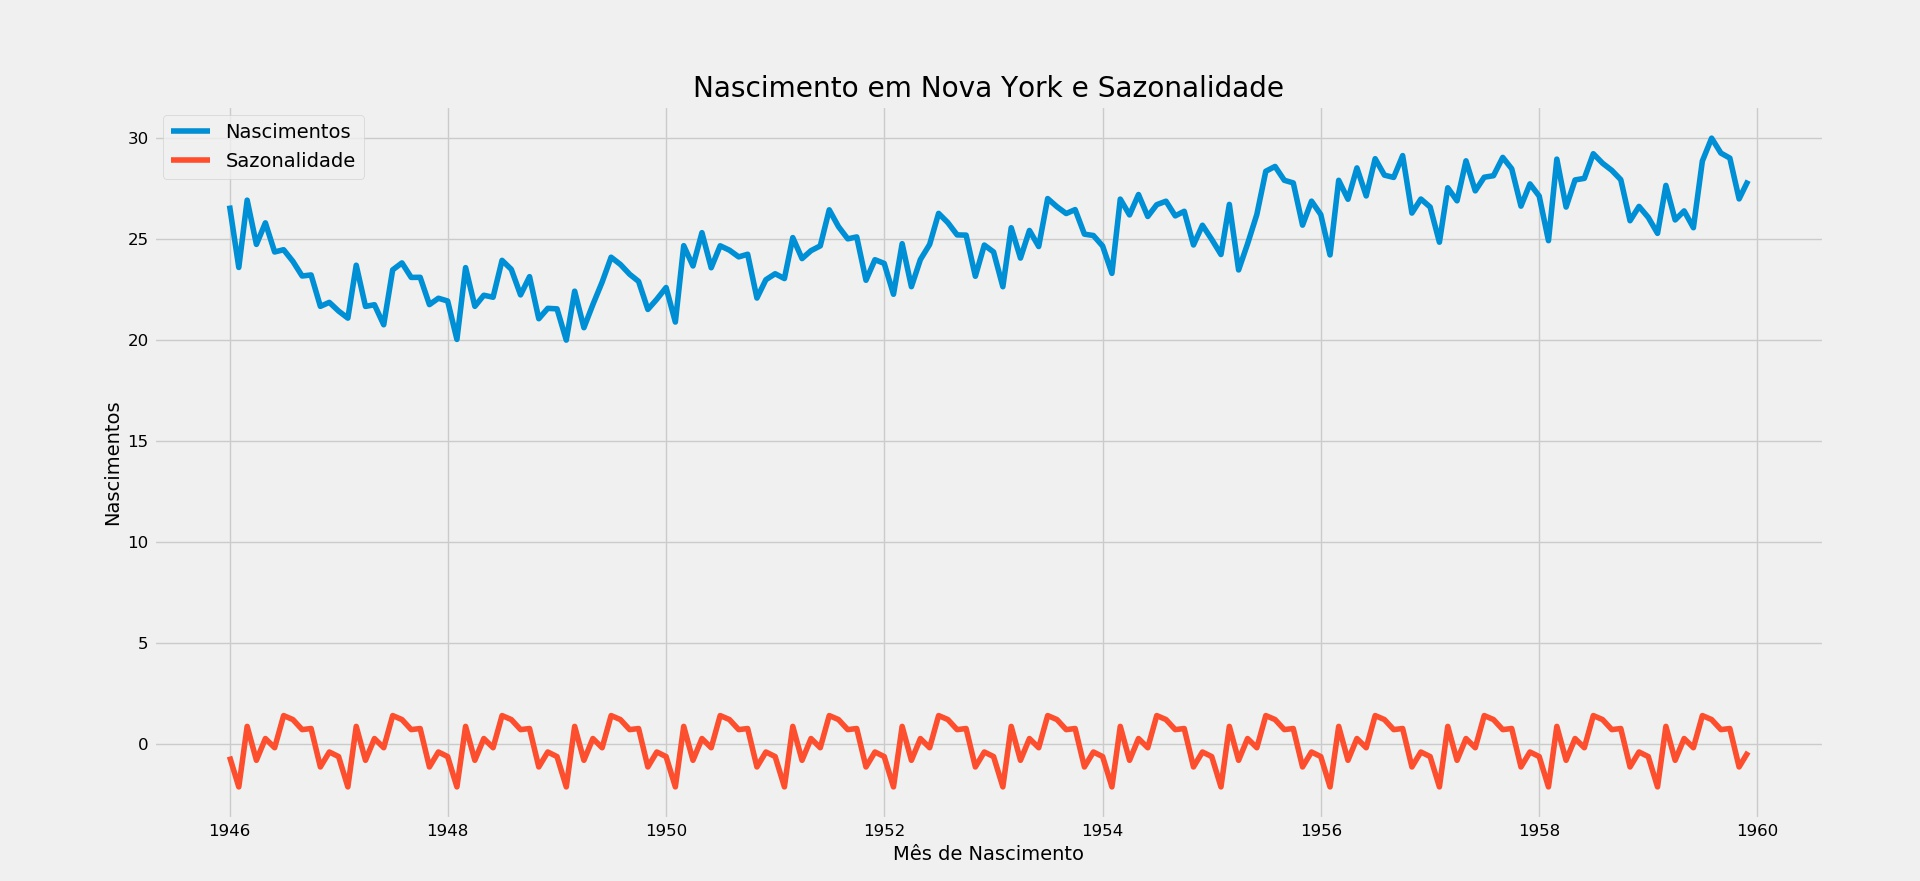
\includegraphics[width=\textwidth]{exemplo2_sazonalidade.jpg}
				
				\caption[\small{Extra��o de sazonalidade com periodicidade anual ($P=12$) para o dataset de nascimentos em Nova York\cite{birthNY} }]{\label{bNYsaz} \small{Extra��o de sazonalidade com periodicidade anual ($P=12$) para o dataset de nascimentos em Nova York. Fonte: Newton (1988). \cite{birthNY}}}
				
			\end{center}	
		}
		
	\end{center}
	
\end{figure}


\paragraph{}Tamb�m pode-se obter a informa��o sobre o per�odo atrav�s da observa��o do gr�fico de autocorrela��o, onde picos de magnitude seguindo um padr�o de espa�amento podem indicar a periodicidade da sazonalidade.

\begin{figure}[H]
	\begin{center}
		{
			\begin{center}
				
				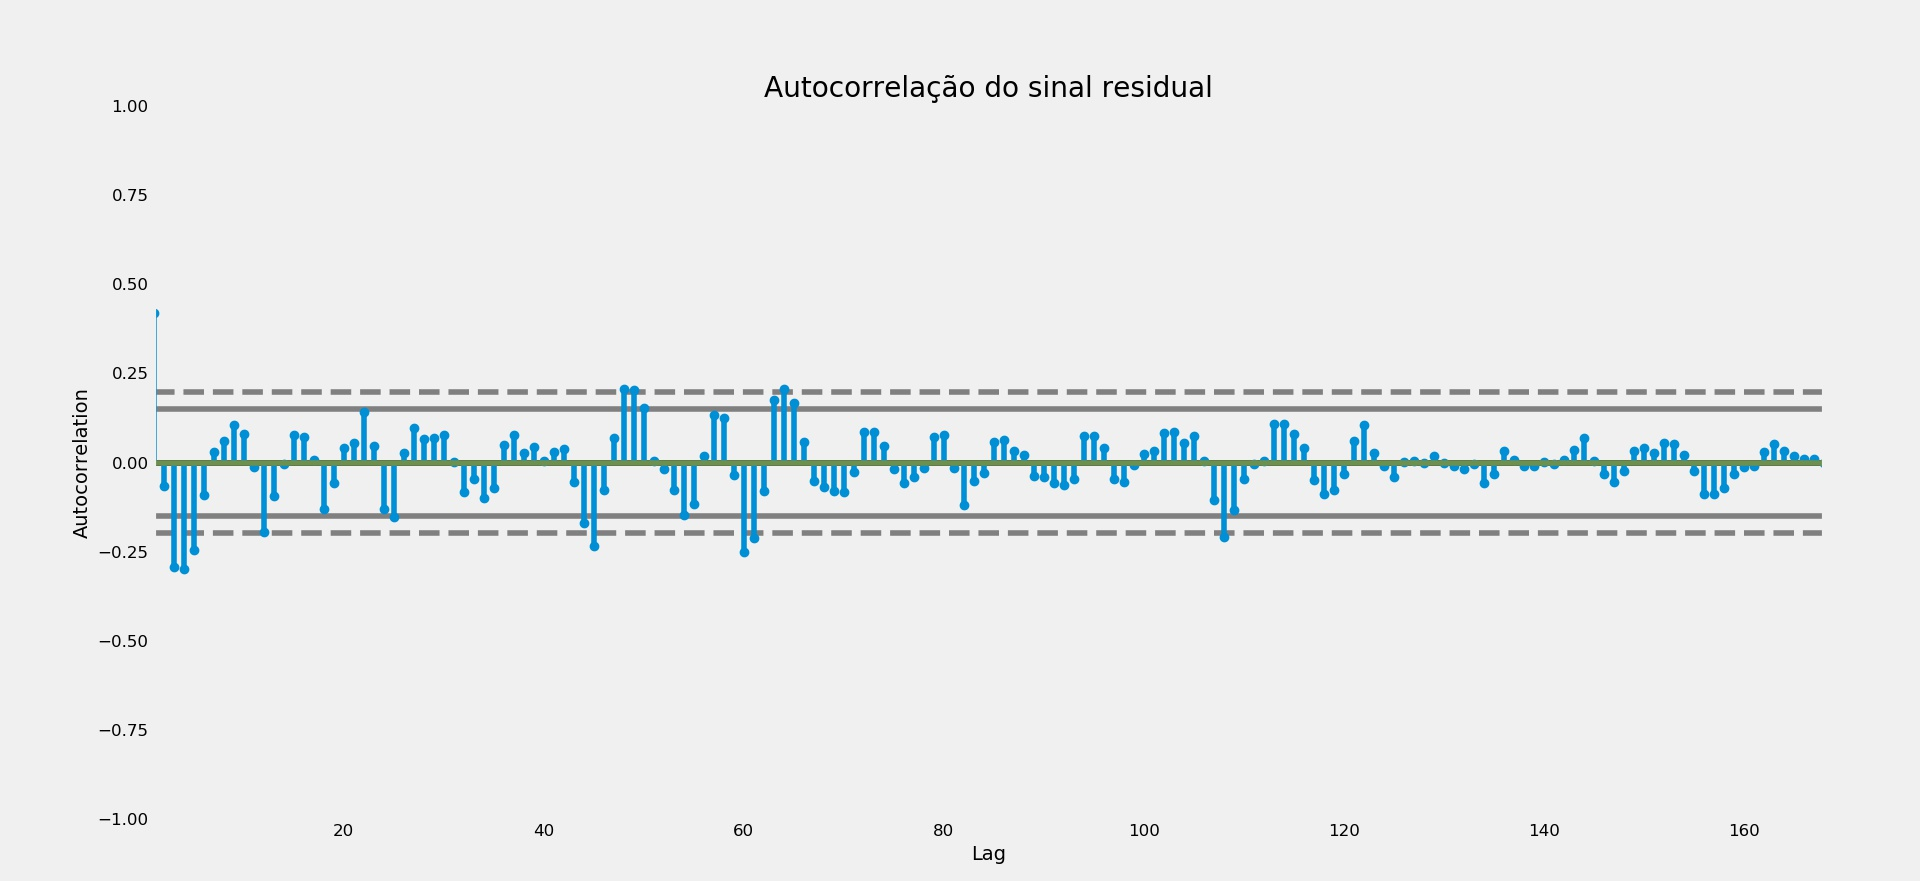
\includegraphics[width=\textwidth]{exemplo2_autocorrelacao.jpg}
				
				\caption[\small{Autocorrela��o para o sinal residual do dataset de nascimentos em Nova York\cite{birthNY} }]{\label{bNYautocorr} \small{Autocorrela��o para o sinal residual do dataset de nascimentos em Nova York. Fonte: Newton (1988). \cite{birthNY}}}
				
			\end{center}	
		}
		
	\end{center}
	
\end{figure}


\subsection{Ciclos Senoidais}
\paragraph{} Os ciclos senoidais representam um caso bem espec�fico de sazonalidade, sendo representados por senoides de per�odo $P$. Essa senoide � extra�da atrav�s da an�lise do espectrograma dado pela FFT-\textit{Fast Fourier Transform}. Os par�metros de s�ida s�o os termos a e b, conforme vistos nas equa��es abaixo\cite{introSP}:

\begin{equation}
cs_t = a \cdot \cos(2\pi f t) + b \cdot \sin(2 \pi f t)
\end{equation}

\paragraph{}Os pontos onde a magnitude do sinal ($\sqrt{a� + b�}$) s�o muito maiores que os outros indicam prov�vel ciclos senoidais que devem ser removidos.

\subsection{Componente Residual} \label{Residuo}
\paragraph{}Caso o processo de extra��o de componentes descrito nos t�picos acima seja realizado com sucesso, ser� obtida uma componente residual estacion�ria. Busca-se tamb�m uma distribui��o pr�xima da normal para facilitar a an�lise. Seguindo esta abordagem, este sinal residual � a �nica parte aleat�ria do modelo. Sendo assim, o problema se reduz a prever o comportamento da parte residual da s�rie temporal.

\begin{figure}[H]
	\begin{center}
		{
			\begin{center}
				
				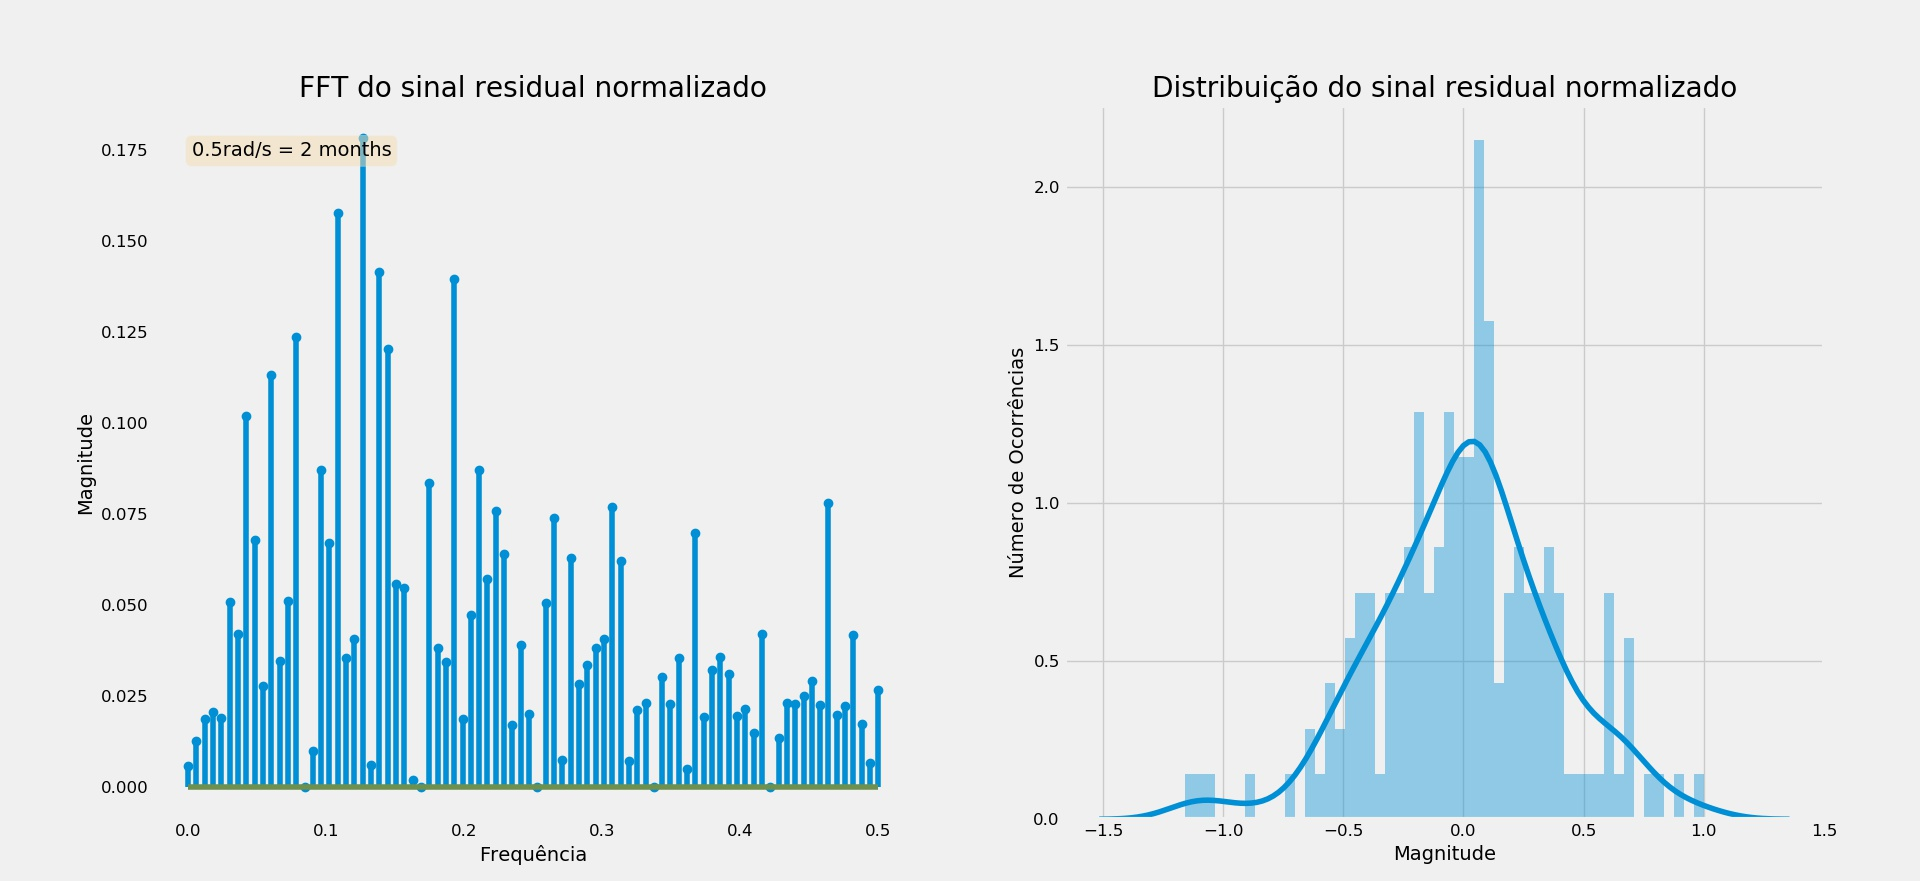
\includegraphics[width=\textwidth]{exemplo2_residual.jpg}
				
				\caption[\small{Residuo sem remo��o de ciclos senoidasi para o dataset de nascimentos em Nova York\cite{birthNY} }]{\label{bNYres} \small{Res�duo sem remo��o de ciclos senoidais para o dataset de nascimentos em Nova York. Fonte: Newton (1988). \cite{birthNY}}}
				
			\end{center}	
		}
		
	\end{center}
	
\end{figure}

\begin{figure}[H]
	\begin{center}
		{
			\begin{center}
				
				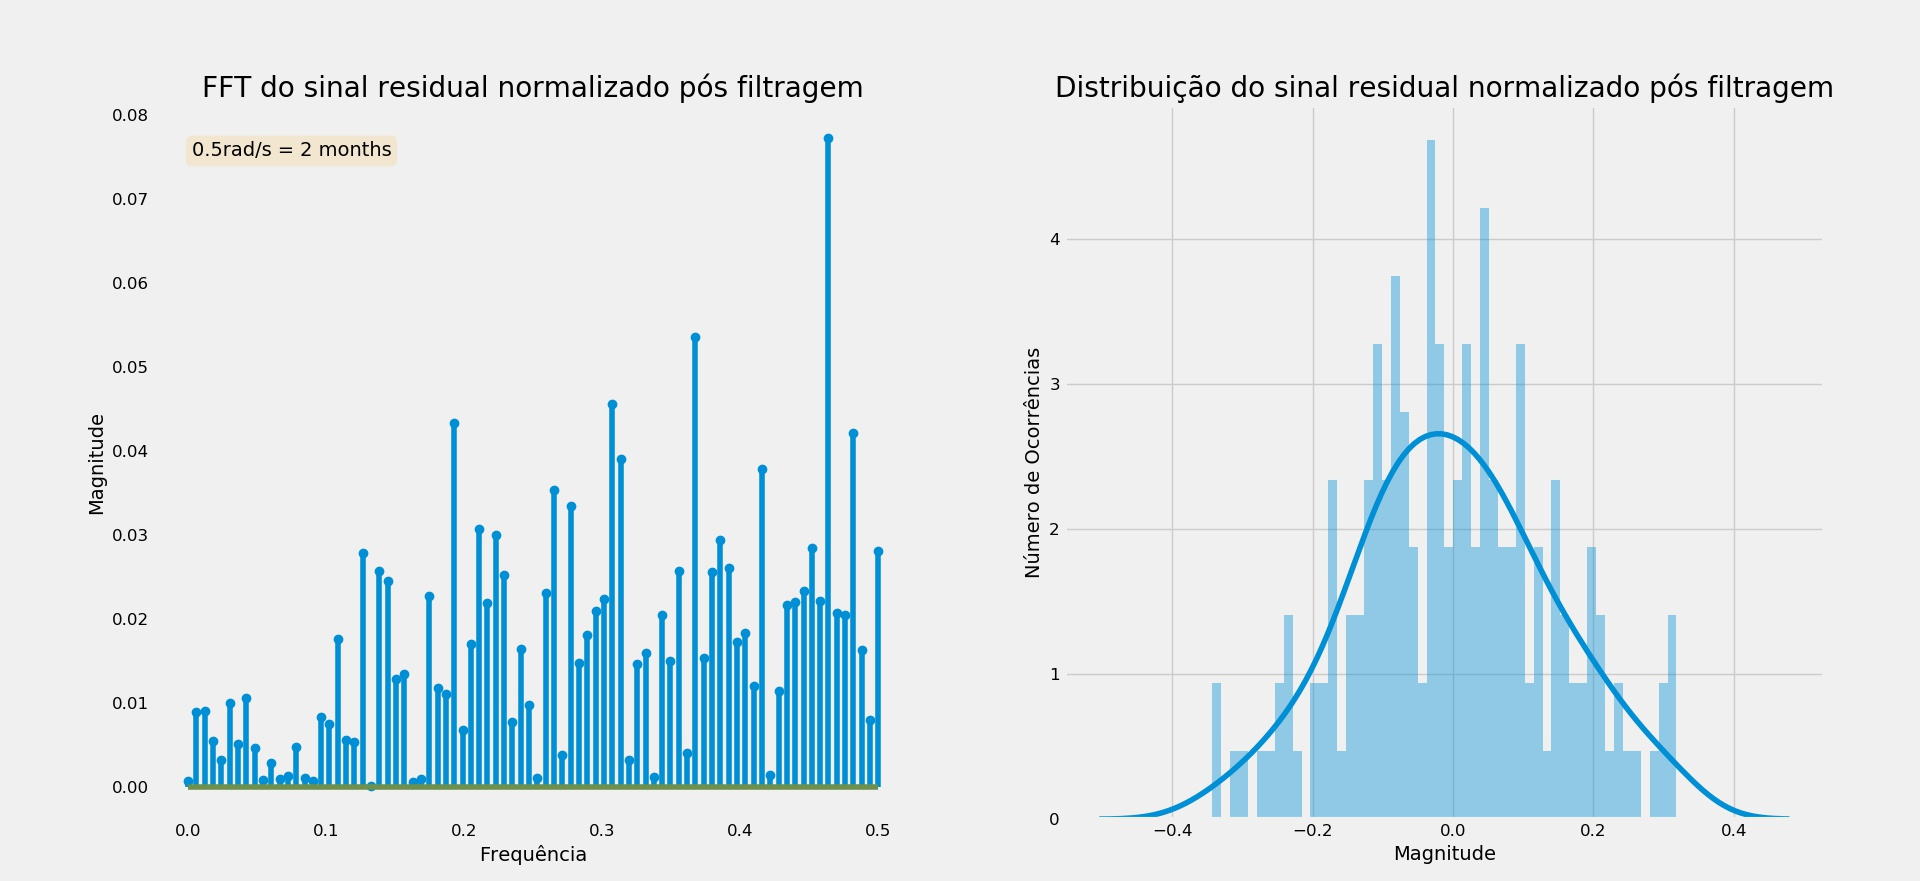
\includegraphics[scale=0.3]{exemplo2_residual_filtrado.jpg}
				
				\caption[\small{Residuo com remo��o de ciclos senoidas para o dataset de nascimentos em Nova York. Filtro Notch com $\omega_0 = 0.135rad\\amostra$ e $Q=0.2$ \cite{birthNY} }]{\label{bNYresFilt} \small{Residuo com remo��o de ciclos senoidais para o dataset de nascimentos em Nova York. Fonte: Newton (1988). \cite{birthNY}}}
				
			\end{center}	
		}
		
	\end{center}
	
\end{figure}


\paragraph{}Como pode-se observar, o sinal residual ap�s a remo��o de ciclos senoidais diminuiu-se a discrep�ncia gerada pelas frequ�ncias pr�ximas de $\omega_0 = 0.135rad\\amostra$ al�m de deixar a distribui��o menos espa�ada (O desvio padr�o mudou de aproximadamente $\sigma=0.37$ para $\sigma=0.14$).

\begin{figure}[H]
	\begin{center}
		{
			\begin{center}
				
				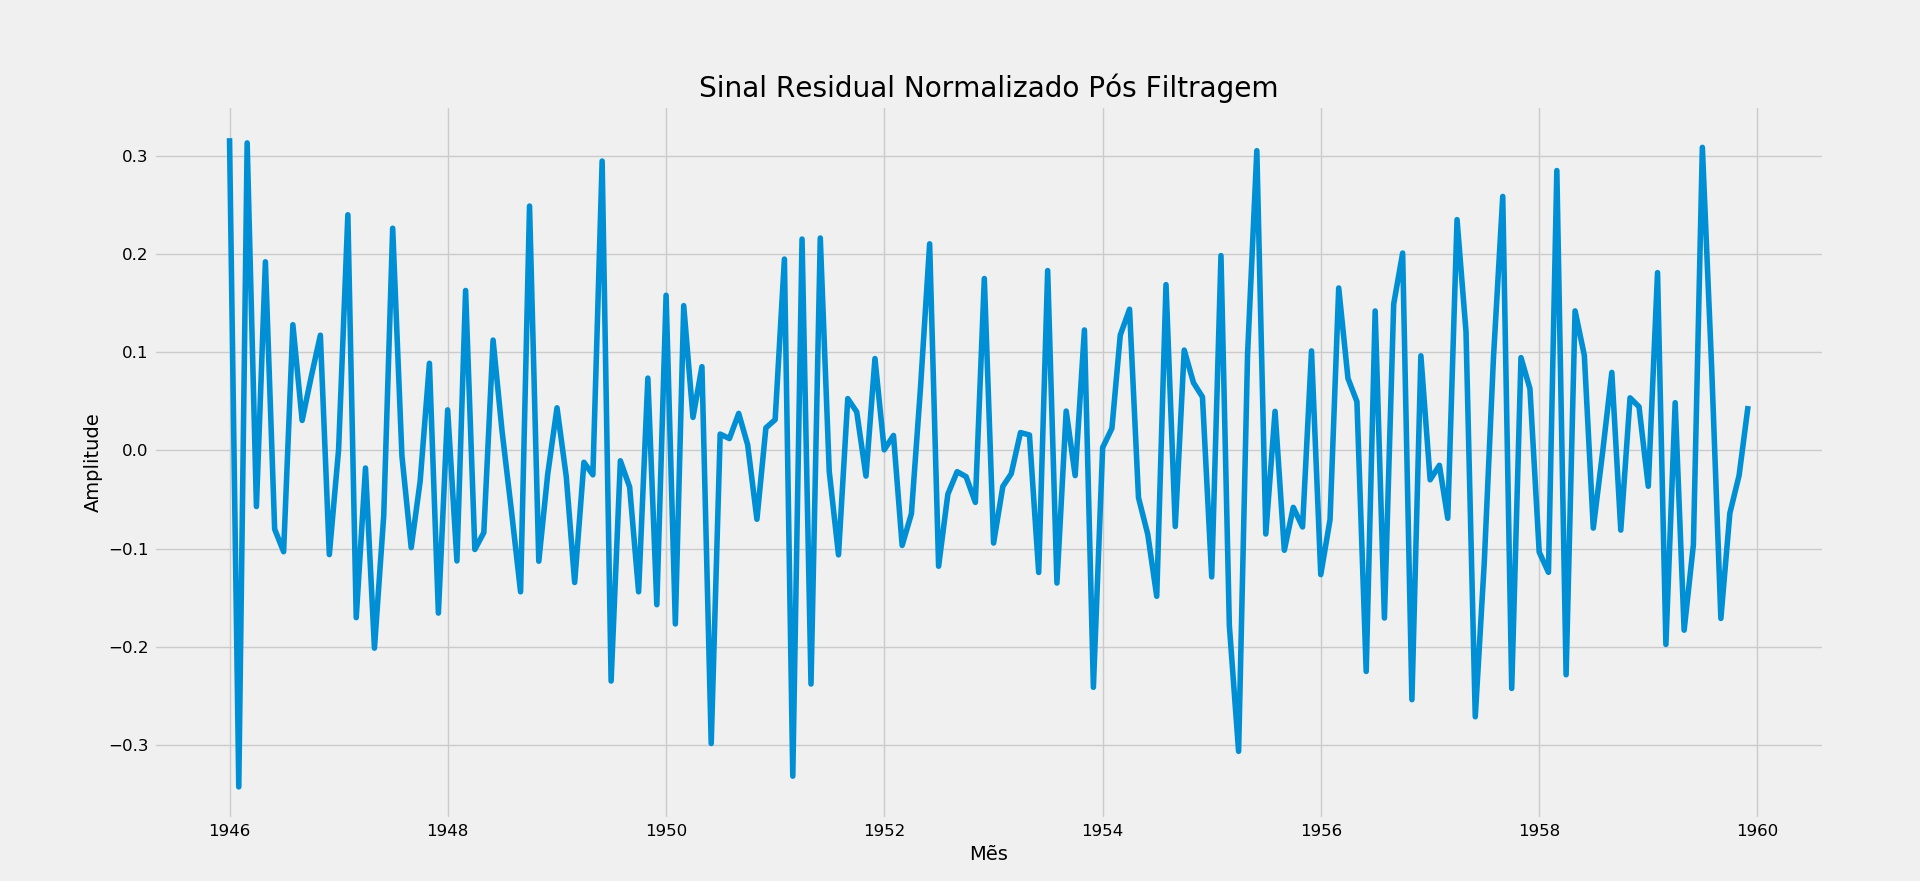
\includegraphics[width=\textwidth]{exemplo2_residual_tempo.jpg}
				
				\caption[\small{Sinal residual no tempo para o dataset de nascimentos em Nova York \cite{birthNY} }]{\label{bNYresFiltTempo} \small{Sinal residual no tempo para o dataset de nascimentos em Nova York Fonte: Newton (1988). \cite{birthNY}}}
				
			\end{center}	
		}
		
	\end{center}
	
\end{figure}


\section{Processamento de Sinais}
\paragraph{}Para remover os ciclos senoidais do espectrograma visto em \ref{bNYres} � necess�rio realizar algum tipo de filtragem sobre sinal. Uma das formas de se classificar um filtro � pela sua resposta em frequ�ncia, sendo as mais comuns: passa-baixa, passa-alta, passa-banda e rejeita-banda.

\paragraph{}No problema de remo��o de ciclos senoidais, busca-se um filtro que remova somente a frequ�ncia com maior magnitude, sem afetar muito as magnitudes das outras frequ�ncias presentes no espectrograma. Para isso procura-se um filtro que seja rejeita-banda com a banda de rejei��o bem estreita e banda de passagem aproximadamente plana.

\paragraph{}Um filtro bastante conhecido na literatura que atende a esse crit�rio � o Notch. A escolha pela vers�o IIRs se d� pela possibilidade de obter atenua��es maiores e banda de rejei��o mais estreita para um mesma ordem $N$ quando comparado com os filtros FIRs. A fun��o de transfer�ncia do filtro Notch de segunda ordem se d� pela equa��o a seguir: \cite{introSP}:

\begin{equation} \label{notch}
H(z) = b \cdot \frac{1 - 2\cos \omega_0 z^{-1} + z^{-2}}{1 - 2b\cos \omega_0 z^{-1} + (2b - 1) z^{-2}}
\end{equation}

e 

\begin{equation}
b = \frac{1}{ 1 + \beta} = \frac{1}{1 + \frac{\sqrt{1 - G_b�}}{G_b} \tan(\frac{\Delta \omega}{2})}
\end{equation}


\paragraph{}Onde $\omega_0$ � a frequ�ncia que se deseja rejeitar, $\Delta \omega$ � a banda de rejei��o, $G_b$ � a atenua��o na frequ�ncia de corte. Geralmente utiliza-se $G_b = 3dB$. O par�metro $Q$ citado na se��o \ref{Residuo} pode ser definido tamb�m como $Q = \frac{\omega_0}{bw}$. $bw$ por sua vez � a banda de rejei��o do filtro Notch.

\begin{figure}[H]
	\begin{center}
		{
			\begin{center}
				
				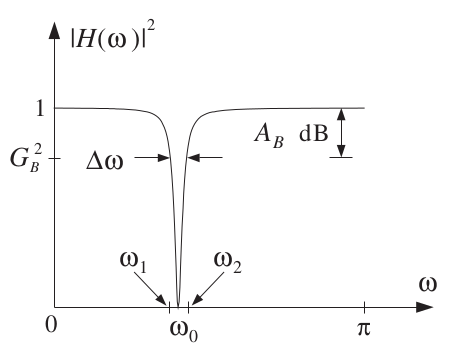
\includegraphics[scale=0.45]{notch.png}
				
				\caption[\small{Filtro Notch IIR digital\cite{introSP} }]{\label{Notch} \small{Filtro Notch IIR digital Fonte: Introduction to Signal Processing. \cite{introSP}}}
				
			\end{center}	
		}
		
	\end{center}
	
\end{figure}

\section{Redes Neurais Artificiais}
\paragraph{}Redes Neurais artificiais s�o modelos computacionais que tentam reproduzir o comportamento observado na estrutura cerebral dos seres vivos. O neur�nio pode ser considerado a c�lula b�sica de processamento do c�rebro humano. Sua estrutura � divida em tr�s partes principais \cite{apostilaCaloba}  \cite{ivan_nunes} \cite{Gurney}:

\begin{figure}[H]
	\begin{center}
		{
			\begin{center}
				
				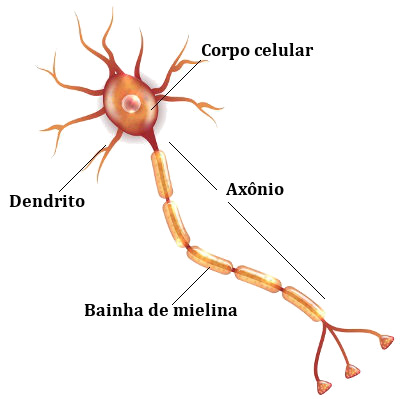
\includegraphics[height=0.25\textheight]{neuronio_biologico.jpg}
				
				\caption[\small{Neur�nio \cite{neuronio} }]{\label{neuronio_biologico} \small{Neur�nio. Fonte: \cite{neuronio}}}
				
			\end{center}	
		}
		
	\end{center}
	
\end{figure}

\begin{itemize}
	\item {\textbf{Dendritos: } S�o respons�veis por receber est�mulos el�tricos de outros neur�nios}
	\item {\textbf{Corpo celular: } Processa as informa��es recebidas pelos dendritos e determina se ser� disparado um impulso el�trico}
	\item {\textbf{Ax�nio: } Transmite o impulso el�trico, e, atrav�s das sinapses, envia a informa��o para outros neur�nios. Isto ocorre sem contato entre os mesmos.}
\end{itemize}

\paragraph{}A representa��o matem�tica desse modelo � dada pela seguinte estrutura:
\begin{figure}[H]
	\begin{center}
		{
			\begin{center}
				
				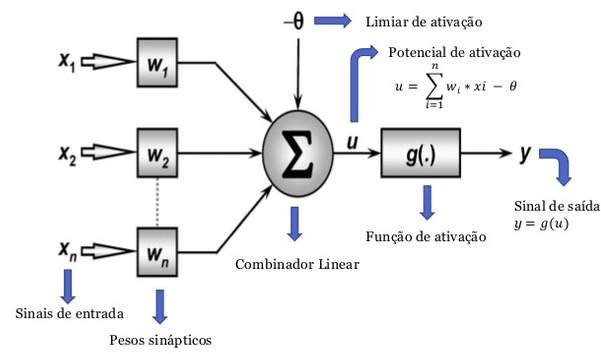
\includegraphics[width=0.8\textwidth]{neuronio_artificial.jpg}
				
				\caption[\small{Neur�nio \cite{neuronio_artificial} }]{\label{neuronio_artificial} \small{Neur�nio Artificial. Fonte: \cite{neuronio_artificial}}}
				
			\end{center}	
		}
		
	\end{center}
	
\end{figure}


\paragraph{}A entrada do neur�nio � um vetor $X = [x_1, x_2 ..., x_n]$
an�logo ao sinais el�tricos transmitidos no c�rebro humano. Essa entrada � ponderada por um conjunto de pesos $W = [w_1, w_2, ..., w_N]$ e somada em um combinador linear junto com um limiar de ativa��o $\theta$. O somat�rio das entradas gera um potencial de ativa��o $u$, o qual passa por uma fun��o de ativa��o e gera um sinal de sa�da que poder� ser propagado para outros neur�nios \cite{ivan_nunes}. As informa��es descritas acima se resumem nas seguintes equa��es \cite{mlp_book}:

\begin{equation} \label{eq_neuronio}
 u_j = \sum_{i = 1}^{N} w_{ji} \cdot x_i - \theta
\end{equation}

\begin{equation}
y = g(u)
\end{equation}

\paragraph{}Sendo que se considerar $x_0 = 1$ e $w_0 = -\theta$, pode-se definir a equa��o \ref{eq_neuronio} como:

\begin{equation}
u = \sum_{i = 0}^{n} w_i \cdot x_i
\end{equation}

\paragraph{}A fun��o de ativa��o pode ter diferentes formatos. Caso seja identidade, obt�m se um regressor linear \cite{Bishop}. Este tipo de abordagem traz uma grande desvantagem, pois a sa�da do sistema sempre ser� linear. Isto vem do fato de que uma composi��o de transforma��es lineares � tamb�m uma transforma��o linear. Sendo assim, nas redes neurais s�o utilizadas fun��es n�o-lineares. Alguns exemplos s�o:
\begin{itemize}
	\item {\textbf{Fun��o Log�stica: } 
		\begin{equation} \label{func_logistica}
			g(u) = \frac{1}{1 + e^{-\beta u}}
		\end{equation}
		Onde $\beta$ � uma constante real que modifica a inclina��o da reta.
	}

\begin{figure}[H]
	\begin{center}
		{
			\begin{center}
				
				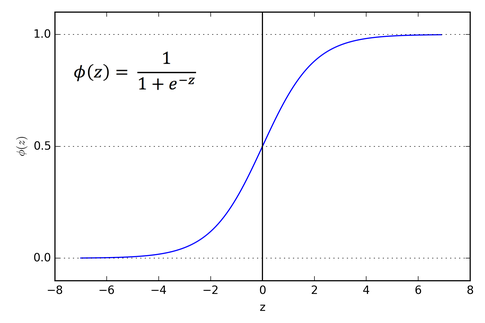
\includegraphics[width=0.5\textwidth]{logistic_func.jpg}
				
				\caption[\small{Fun��o log�stica \cite{funcoes_ativacao} }]{\label{logistic_func} \small{Neur�nio Artificial. Fonte: \cite{funcoes_ativacao}}}
				
			\end{center}	
		}
		
	\end{center}
	
\end{figure}
	\item {\textbf{Tangente Hiperb�lica: }
		\begin{equation} \label{func_tanh}
			g(u) = \frac{1 - e^{-\beta u}}{1 + e^{-\beta u}}
		\end{equation}
		Onde $-1 \leq g(u) \leq$ para qualquer u e assim como em \ref{func_logistica}, $\beta$ tamb�m modifica a inclina��o da reta.
	}

\begin{figure}[H]
	\begin{center}
		{
			\begin{center}
				
				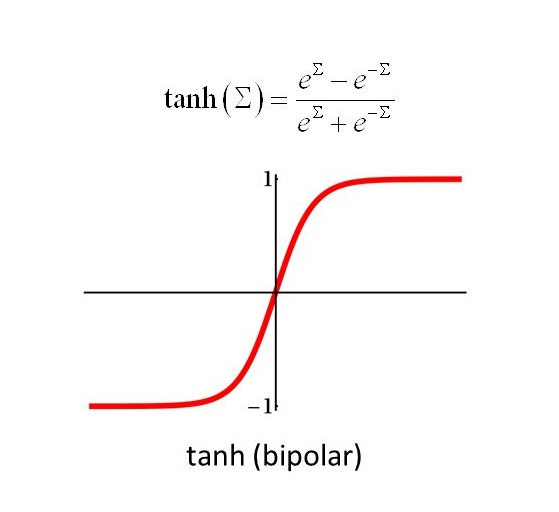
\includegraphics[width=0.5\textwidth]{tanh.jpg}
				
				\caption[\small{Tangente hiberb�lica \cite{tanh} }]{\label{tanh} \small{Tangente Hiperb�lica. Fonte: \cite{tanh}}}
				
			\end{center}	
		}
		
	\end{center}
	
\end{figure}


	\item {\textbf{Unidade Linear Retificada - ReLU \cite{K_He}:}
		\begin{equation} \label{func_relu}
			g(u) = \max(0, u)
		\end{equation}
		Esta fun��o � linear na parte positiva e zero na parte negativa.
	}

\begin{figure}[H]
	\begin{center}
		{
			\begin{center}
				
				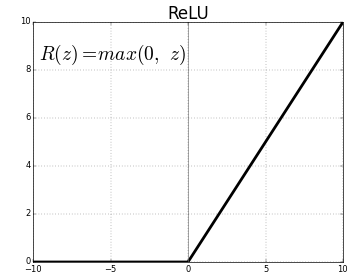
\includegraphics[width=0.5\textwidth]{relu.jpg}
				
				\caption[\small{ReLU \cite{relu} }]{\label{relu} \small{ReLU. Fonte: \cite{relu}}}
				
			\end{center}	
		}
		
	\end{center}
	
\end{figure}


\end{itemize}

\paragraph{}As fun��es de ativa��o \ref{func_logistica} e \ref{func_tanh} s�o deriv�veis em todos os pontos e a \ref{func_relu} s� n�o � deriv�vel no ponto zero, por�m contorna-se essa limita��o fazendo $g'(0) = 0$. A ReLU tem sido essencial para o estado da arte de redes neurais \cite{relu} \cite{deep_learning_relu} \cite{relu_recomender} \cite{deep_learning_relu2}. A derivada da fun��o de ativa��o � utilizada pelos algoritmos de treinamento baseados no gradiente do erro assim como ser� visto mais � frente.

\subsection{Backpropagation}
\paragraph{}O algoritmo de backpropagtion � bastante utilizado no treinamento de de redes neurais e utiliza o gradiente do erro como base dos c�lculos, assim como mencionado anteriormente \cite{Bishop} \cite{backprop}. Busca-se mover o vetor dos pesos na dire��o do m�nimo local. A express�o de atualiza��o dos pesos � da seguinte forma:
\begin{equation} \label{grad_desc}
 w^{(\tau + 1)} = w^{(\tau)} - \eta\nabla E_n w^{(\tau)}
\end{equation}

\paragraph{}O qual deve ser repetido at� que o erro se torne suficientemente pequeno. O gradiente do erro nessa f�rmula � dado por:

\begin{equation}
\nabla E^{(\tau)} = \frac{\partial E}{\partial W_{ji}^{(\tau)}} = \frac{\partial E}{\partial Y_{j}^{(\tau)}} \cdot \frac{\partial Yj^{(\tau)}}{\partial u_j^{(\tau)}} \cdot \frac{\partial u_j^{(\tau)}}{\partial W_{ji}^{(\tau)}}
\end{equation}

\paragraph{}T�m-se como ideia principal do mesmo avaliar quanto que um determinado peso em uma camada influ�ncia no erro da sa�da e assim, modific�-lo de forma a tornar esse erro menor. Um ponto importante para o sucesso do algoritmo � a normaliza��o da entrada, visto que diminui o tempo de converg�ncia.

\begin{figure}[H]
	\begin{center}
		{
			\begin{center}
				
				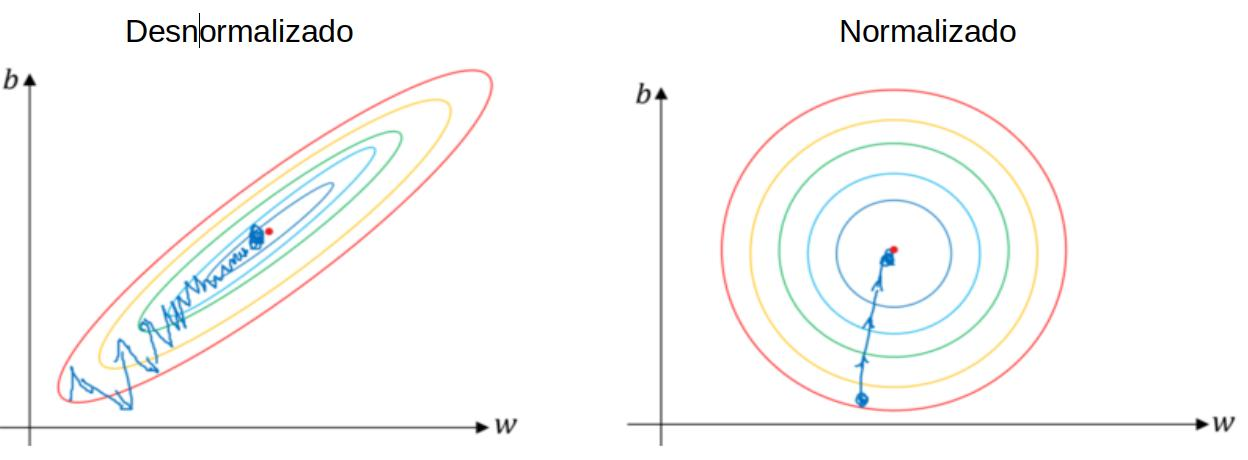
\includegraphics[width=\textwidth]{grad_desc.jpg}
				
				\caption[\small{Tangente hiberb�lica \cite{relu} }]{\label{grad_desc_fig} \small{Gradiente Descendente desnormalizado e normalizado. Fonte: \cite{relu}}}
				
			\end{center}	
		}
		
	\end{center}
	
\end{figure}

\subsection{Rede perceptron multicamadas - MLP}
\paragraph{}Assim como no c�rebro, os neur�nios artificiais podem ser agrupados em estrutura mais complexas. Para uma camada inicial com N entradas t�m se na J-�sima sa�da:
\begin{equation}
Y_{j}^{(1)} = g(\sum_{i = 0}^{N} W_{ji}^{(1)} \cdot X_i)
\end{equation}

\paragraph{}Nas camadas seguintes utiliza-se a sa�da da camada anterior (com $M$ neur�nios) como entrada na camada atual. Na f�rmula busca-se obter a sa�da para o $P$-�simo neur�nio da camada $H$. 
\begin{equation}
Y_{P}^{(H)} = g(\sum_{i = 0}^{M} W_{pi}^{(H)} \cdot Y_{i}^{(H-1)})
\end{equation}

\paragraph{}As redes MLP tem sido utilizadas em diferentes classes de problemas como classifica��o de elementos e previs�o de s�ries temporais \cite{apostilaCaloba} \cite{ivan_nunes}  \cite{mlp_atmosfera}. Com o grande crescimento do n�mero de dados dispon�vel para utiliza��o e o desenvolvimento das tecnologias computacionais, t�m-se atualmente redes com muitas camadas e neur�nios em busca de obter maior capacidade de separa��o, previs�o, al�m de poder obter informa��es relevantes sobre neur�nios intermedi�rios da rede \cite{deep_learning1} \cite{deep_learning_book} \cite{microsoft_dl}.

\begin{figure}[H]
	\begin{center}
		{
			\begin{center}
				
				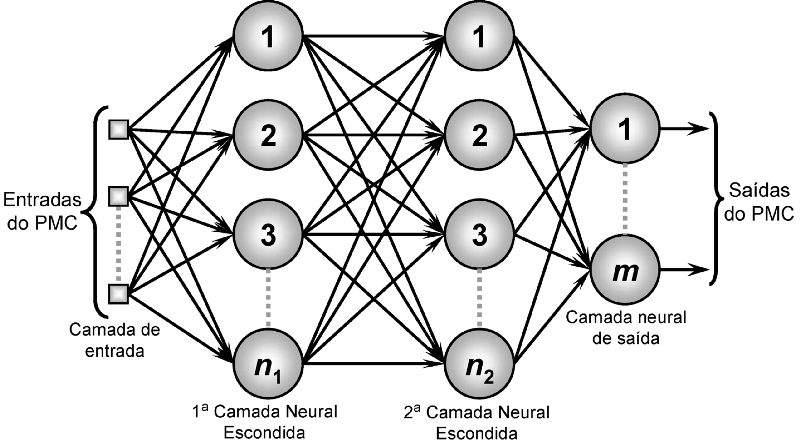
\includegraphics[width=0.7\textwidth]{mlp.jpg}
				
				\caption[\small{Rede Perceptron Multicamadas \cite{relu} }]{\label{mlp} \small{Rede Perceptron Multicamadas. Fonte: \cite{mlp}}}
				
			\end{center}	
		}
		
	\end{center}
	
\end{figure}

\subsection{Treinamento}
\paragraph{}Para que a rede consiga de fato "aprender" com os dados � necess�rio realizar o treinamento. Para que o mesmo seja bem sucedido deve-se atentar para alguns fatores como: 
\begin{itemize}
	\item {\textbf{Inicializa��o dos pesos: }Os pesos n�o devem se iniciados com o mesmo valor, pois isto faria com que cada neur�nio interprete a entrada da mesma forma, gerando ent�o uma estrutura sim�trica \cite{relu} \cite{yam} \cite{ryanhsiao}}.
	
	\item {\textbf{Fun��o custo: } H� necessidade de definir qual fun��o de custo ser� utilizada na avalia��o dos resultados da rede. A fun��o mais comum � o erro m�dio quadr�tico - \textit{MSE}, por�m dependendo da an�lise que se deseja fazer e do problema a ser resolvido, outras fun��es podem ser utilizadas como a o erro m�dio quadr�tico - \textit{RMSE}, erro absoluto -\textit{MAE} e acur�cia - \textit{ACC} \cite{tccDanilo}}.
		
	\item {\textbf{Curva de aprendizado: }� comum tamb�m utilizar um gr�fico do erro na sa�da em fun��o da �poca de treinamento para o conjunto de treinamento e valida��o. Atrav�s do mesmo � poss�vel observar caracter�sticas como overfitting e underfitting e selecionar o conjunto de pesos que tem o melhor compromisso \cite{data_overfit}.}
		
	\item {\textbf{Quantidade de dados $X$ complexidade da rede: } Outro fator importante a ser observado � a quantidade de dados dispon�vel para treinamento, visto que quanto maior a complexidade estrutural da rede, maior a capacidade de gerar fun��es complexa, portanto torna-se necess�rio uma maior quantidade de dados para que a mesma seja treinada sem o efeito de overfitting.}
	
	\item {\textbf{Taxa de aprendizado: }Caso o fator $\eta$ da f�rmula \ref{grad_desc} seja um valor muito grande, o algoritmo n�o conseguir� convergir para um m�nimo, por�m se $\eta$ for um n�mero muito grande, o treinamento pode levar muita �pocas at� convergir. Cabe ent�o a quem especifica os par�metros da rede neural escolher um $\eta$ adequado de forma com que a converg�ncia ocorra e n�o demore demais.}
	\begin{figure}[H]
		\begin{center}
			{
				\begin{center}
					
					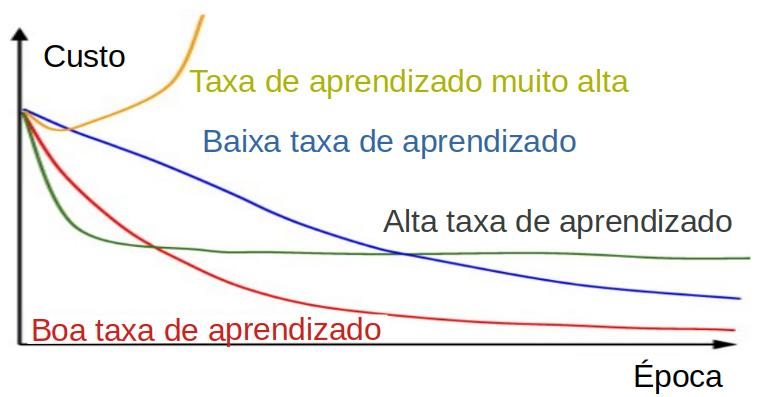
\includegraphics[width=0.7\textwidth]{learning_rate.jpg}
					
					\caption[\small{Influ�ncia da taxa de aprendizado \cite{grad_desc} }]{\label{l_rate} \small{Influ�ncia da taxa de aprendizado. Fonte: \cite{grad_desc}}}
					
				\end{center}	
			}
			
		\end{center}
		
	\end{figure}
	
	\item {\textbf{Divis�o dos dados de entrada: }Uma pr�tica comum para se obter resultados consistentes � dividir os dados em um conjunto de testes e outro de valida��o, de forma que o conjunto de testes n�o seja usado no treinamento, sendo assim usado para verificar o qu�o bom s�o os resultados da rede para dados desconhecidos. Outra pr�tica comum � dividir o conjunto de treinamento em treino e valida��o e utilizar a valida��o cruzada, de forma a realizar v�rios treinos com a mesma arquitetura, permitindo obter melhores resultados no treinamento  \cite{crossValidation}.}
		\begin{figure}[H]
		\begin{center}
			{
				\begin{center}
					
					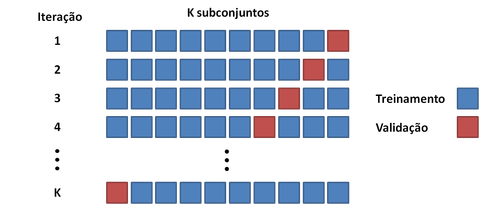
\includegraphics[width=0.7\textwidth]{validacao_cruzada.jpg}
					
					\caption[\small{Validacao Cruzadas \cite{validacao_cruzada} }]{\label{validacao_cruzada} \small{Valida��o cruzada. Fonte: \cite{validacao_cruzada}}}
					
				\end{center}	
			}
			
		\end{center}
		
	\end{figure}
	


\end{itemize}





% ---------------------------------------------------------------
% Chapter 6 - Conclus�es
% ---------------------------------------------------------------
\chapter{Conclus�es}
\label{cap6}
 \paragraph{}Neste trabalho foi proposto um modelo baseado em redes neurais, com o objetivo de prever o valor m�dio do PLD para alguns meses a frente. Para isso, foi necess�ria a decomposi��o do sinal, deixando para o treinamento da rede somente a parte n�o-determin�stica. Foram testados diferentes m�todos de extra��o das componentes at� chegar na que foi utilizada no Cap�tulo 5. Al�m disso, as MLPs foram treinadas para quantidades variadas de neur�nios na camada intermedi�ria, buscando a melhor arquitetura que solucionasse o problema proposto.
 
  \paragraph{}Ao final do projeto, obteve-se um m�todo de sele��o do n�mero de neur�nios para MLPs com uma camada escondida e quantidade de dados reduzida. Al�m disso, a pr�pria extra��o das componentes, pode trazer valor se analisada com cuidado, pois a tend�ncia, sazonalidade e ciclos senoidais podem a ajudar no entendimento dos fen�menos observado na curva do PLD.
 
 \paragraph{}Devido ao fato do modelo ter erros de estima��o relativamente elevados, n�o � poss�vel utilizar o mesmo de forma a obter lucro. Apesar disso, pode-se usar o mesmo em outras aplica��es, como por exemplo, an�lise de relev�ncia das vari�veis de entrada. H� tamb�m a possibilidade de realizar previs�es sobre os patamares dos valores, assim como visto na figura \ref{ClassesPrevisao}.
 
 \paragraph{}Quanto �s conclus�es obtidas atrav�s do experimento, observou-se que o erro tem uma tend�ncia crescente conforme o n�mero de meses � frente, assim como esperado. Isso torna cada vez mais complexa a utiliza��o do modelo para cen�rio muito distantes. A aplica��o da rede para corre��o dos erros trouxe para a previs�o um compromisso entre erro m�ximo e m�dio, conforme a arquitetura escolhida.
 
 \paragraph{}Para trabalhos futuros, seria interessante comparar os resultados obtidos com modeos diferentes, como por exemplo, SARIMA e GARCH e ADALASSO. Al�m disso, podem ser exploradas outras formas de extra��o das componentes da s�rie temporal, de forma a obter um sinal residual com menos energia dos que os que foram encontrados.
 
 \paragraph{}Outra abordagem pode ser a de considerar os dados para os anos anteriores 2015 e analisar quanto isso afeta a previs�o do PLD m�dio mensal. Nesse caso, cabe tamb�m utilizar estruturas de redes neurais mais complexas, como por exemplo LSTM - \textit{Long Short-Term Memory}.



% ---------------------------------------------------------------
% Bibliografia
% ---------------------------------------------------------------
\normalsize
\cleardoublepage
\addcontentsline{toc}{chapter}{Bibliografia}
\bibliographystyle{coppe}
\bibliography{biblio}

% ---------------------------------------------------------------
% Ap�ndices 
% ---------------------------------------------------------------
   \appendix
   % ---------------------------------------------------------------
   % Ap�ndice A
   % ---------------------------------------------------------------
   \chapter{O que � um ap�ndice}
   \label{ApendiceA}
   \section{Previs�o para 2 meses � frente}
\begin{figure}[H]
	\begin{center}
		{
			\begin{center}
				
				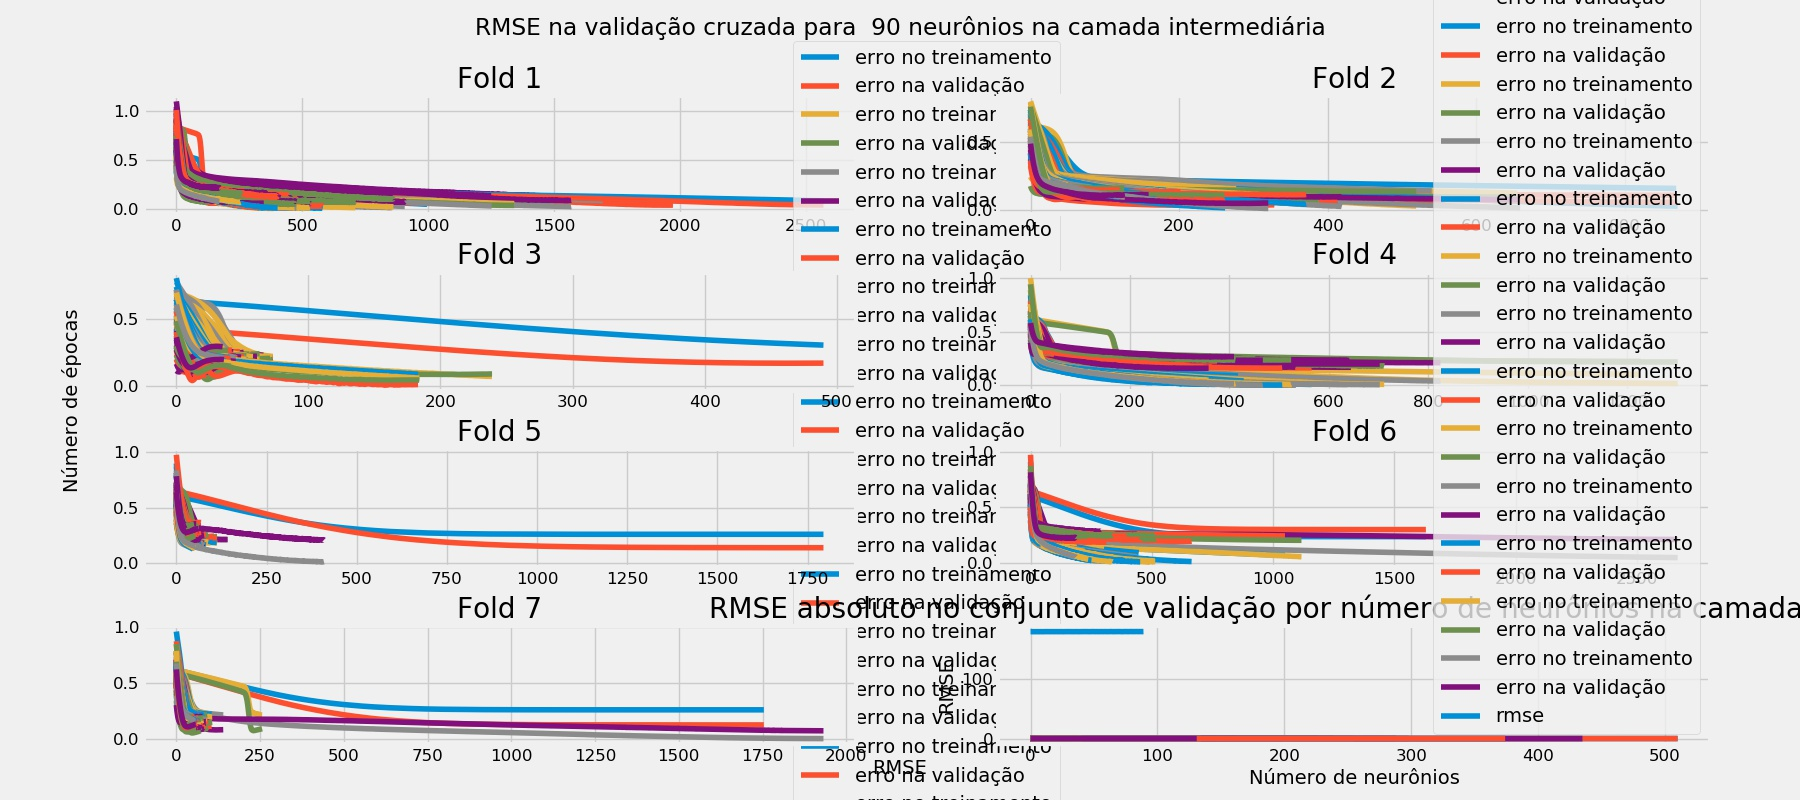
\includegraphics[width=\textwidth]{rmse_val_set_t2.jpg}
				
				\caption[\small{RMSE pelo n�mero de neur�nios no conjunto de valida��o para previs�o do PLD 2 meses � frente.}]{\label{rmseValT2} \small{RMSE pelo n�mero de neur�nios no conjunto de valida��o.}}
				
			\end{center}
		}	
	\end{center}	
\end{figure}


\paragraph{}No conjunto de teste o resultado foi o seguinte:
\begin{figure}[H]
	\begin{center}
		{
			\begin{center}
				
				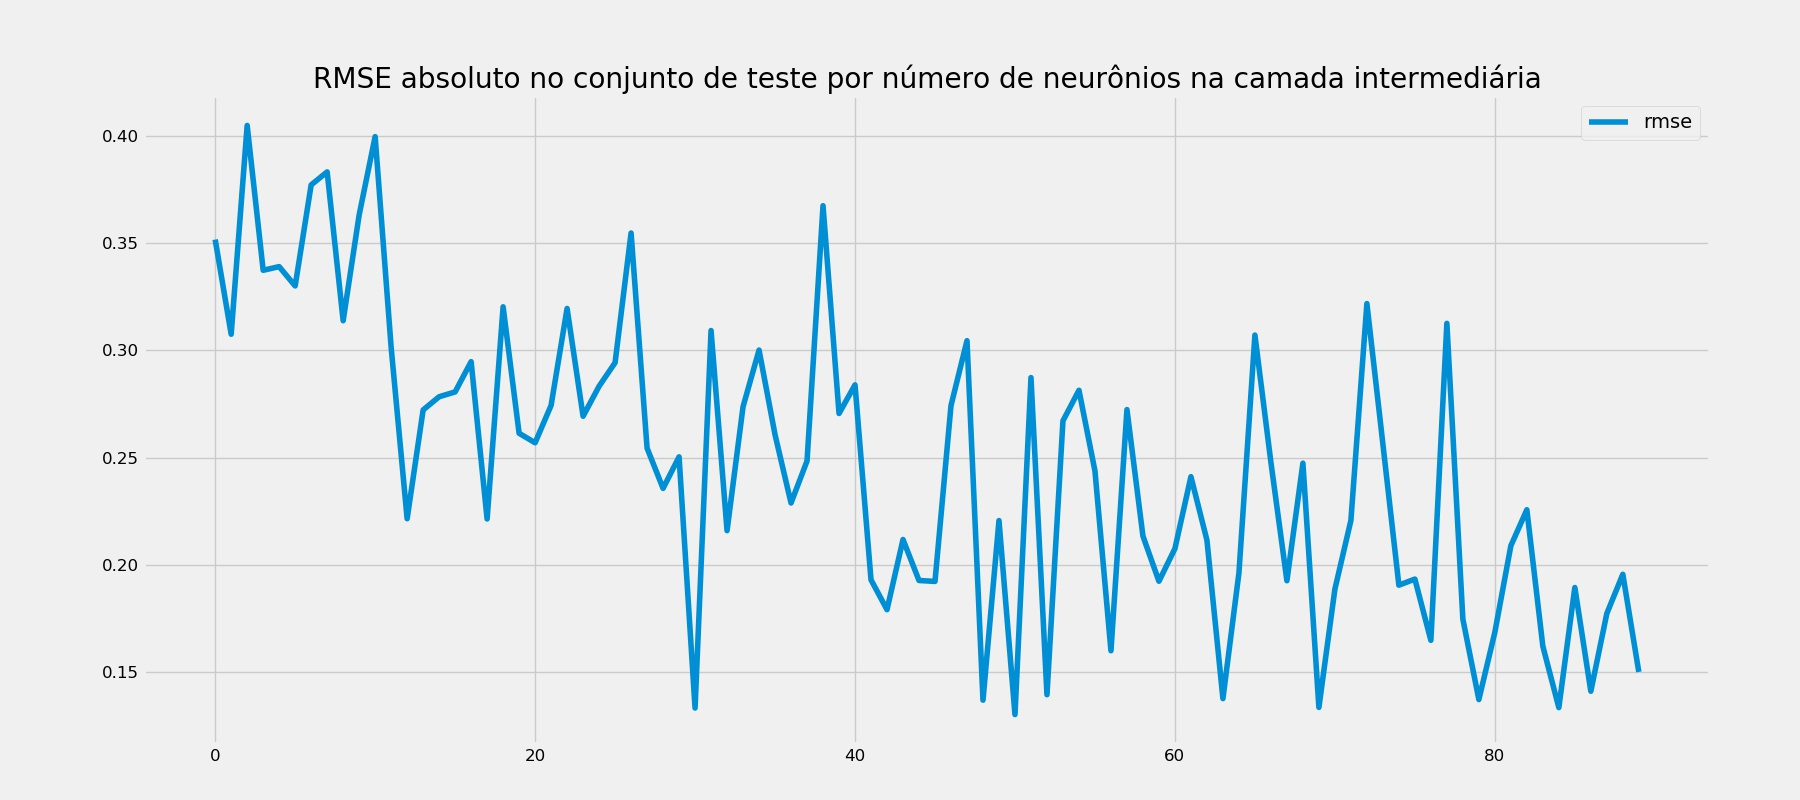
\includegraphics[width=\textwidth]{rmse_test_set_t2.jpg}
				
				\caption[\small{RMSE pelo n�mero de neur�nios no conjunto de teste para previs�o do PLD 2 meses � frente.}]{\label{rmseTestT2} \small{RMSE pelo n�mero de neur�nios no conjunto de teste.}}
				
			\end{center}
		}	
	\end{center}	
\end{figure}


\begin{table}[H]	
	\begin{center}
		\caption{Resultados obtidos com as redes no dataset de valida��o para previs�o do PLD 2 meses � frente.}			
		\begin{tabular}{|c|c|c|c|c|c|c|c|}\hline \label{table:tabelaT2}
			
			\textbf{\#neur�nios} & \textbf{RMSE} & \textbf{STD} & \textbf{$a$ (m�dia)} & \textbf{$\epsilon_1$} & \textbf{$b$ (m�dia)} & \textbf{$\epsilon_2$} & \textbf{$\epsilon_3$}\\ \hline \vspace{-1.0mm}69 & 97,141 & 76,580 & 1,029 & 0,001 & 0,011 & 0,000 & 0,001 \\ \hline
			79 & 96,834 & 84,359 & 0,945 & 0,001 & 0,022 & 0,001 & 0,002 \\ \hline
			42 & 100,878 & 80,880 & 1,056 & 0,001 & -0,022 & 0,001 & 0,002 \\ \hline
			86 & 96,153 & 77,890 & 0,945 & 0,001 & -0,032 & 0,001 & 0,002 \\ \hline
			58 & 108,011 & 83,478 & 1,181 & 0,003 & 0,001 & 0,000 & 0,003 \\ \hline
		\end{tabular}
	\end{center}
\end{table}

\paragraph{}E com isso o modelo com 69 neur�nios foi escolhido. O treinamento dessa estrutura obteve os seguintes erros pelo n�mero de �pocas:

\begin{figure}[H]
	\begin{center}
		{
			\begin{center}
				
				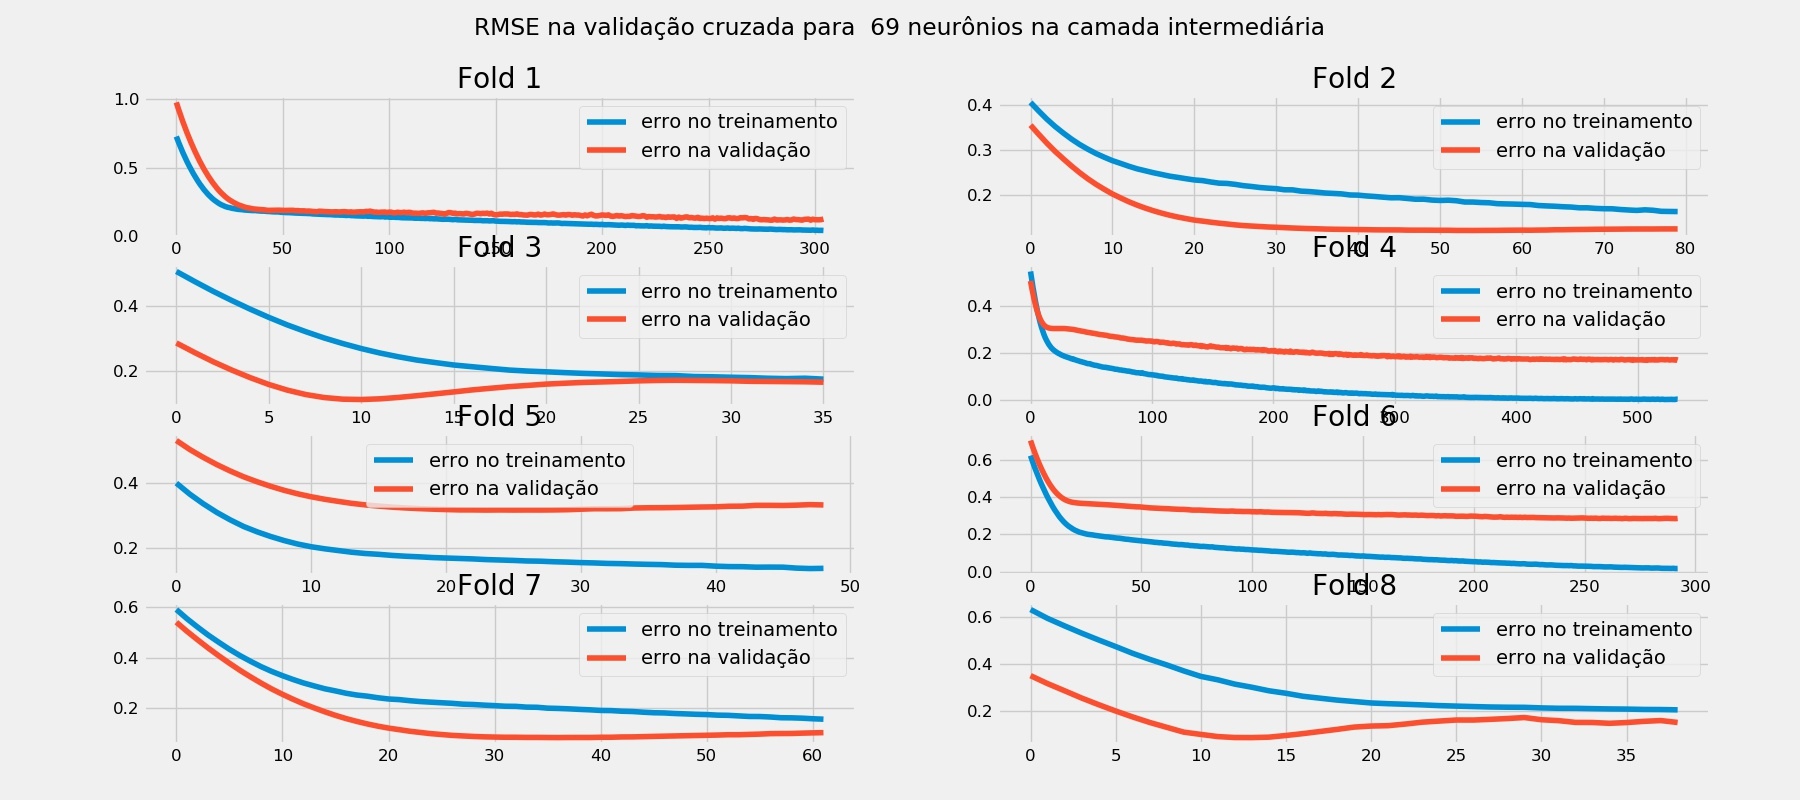
\includegraphics[width=\textwidth]{convergence_t2.jpg}
				
				\caption[\small{Erro pelo n�mero de �pocas e por subconjunto para previs�o do PLD 2 meses � frente.}]{\label{convT2} \small{Erro pelo n�mero de �pocas e por subconjunto para previs�o do PLD 2 meses � frente.}}
				
			\end{center}
		}	
	\end{center}	
\end{figure}


\paragraph{}E obteve-se os seguintes resultados:
\begin{figure}[H]
	\begin{center}
		{
			\begin{center}
				
				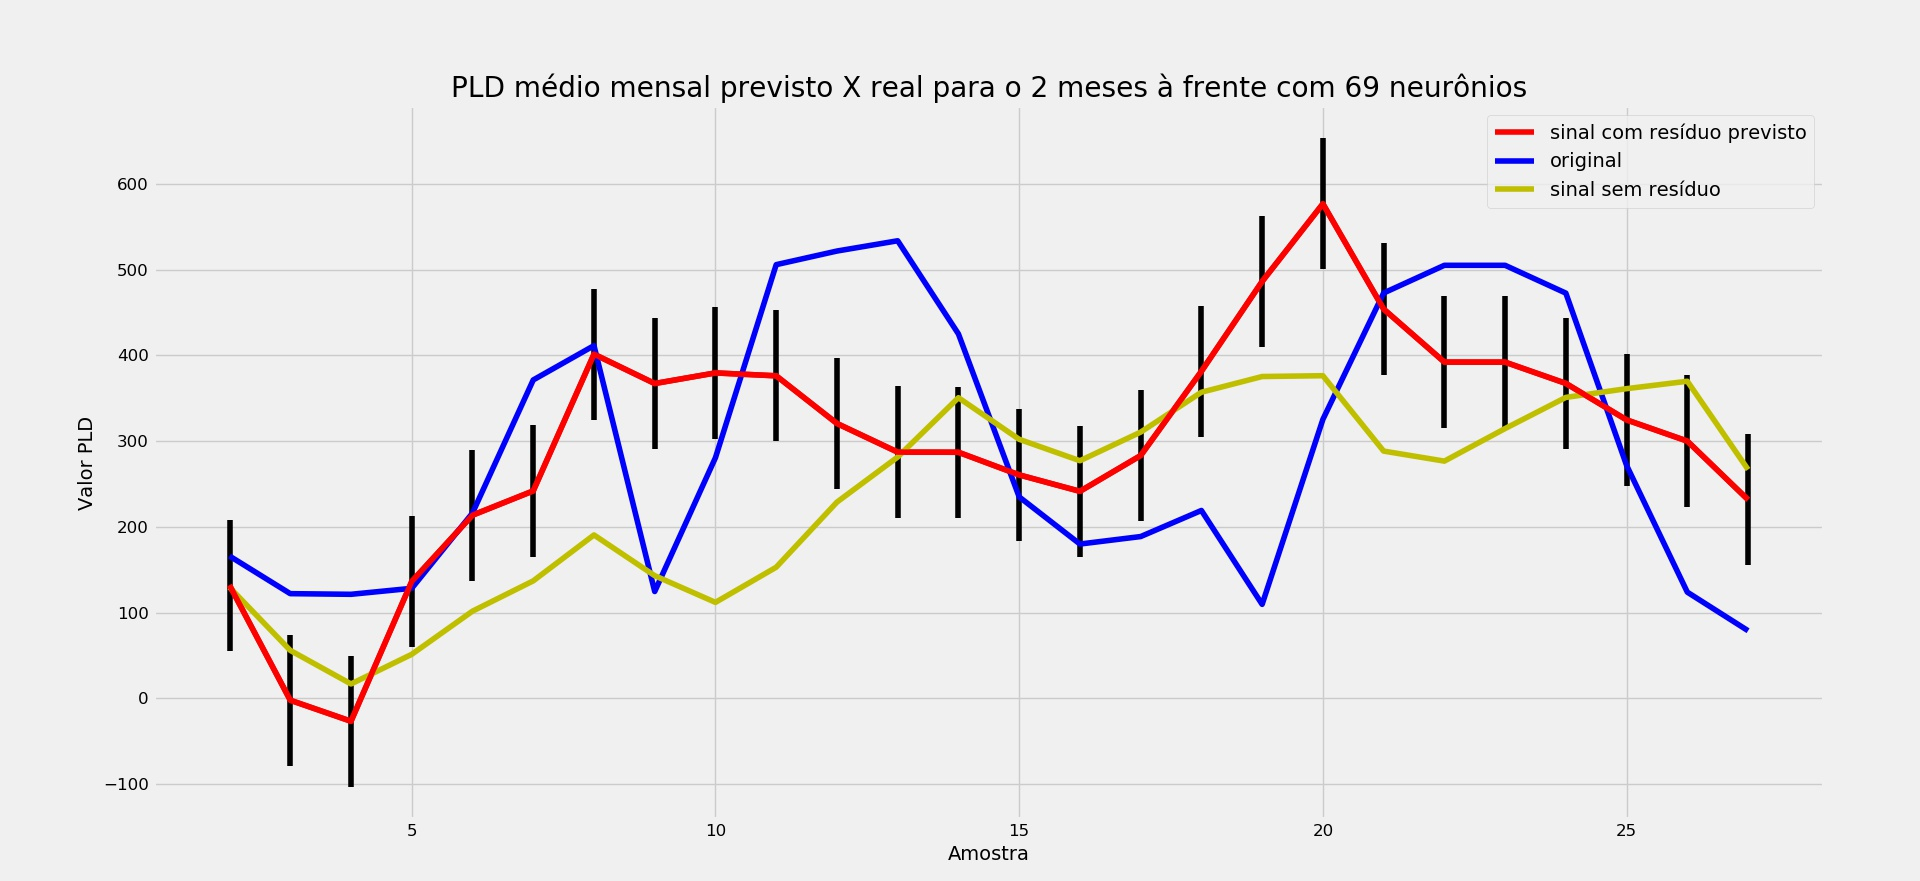
\includegraphics[width=\textwidth]{sinal_completo_t2.jpg}
				
				\caption[\small{Compara��o entre o sinal original e o resultado obtido para previs�o do PLD 2 meses � frente.}]{\label{completoT2} \small{Compara��o entre o sinal original e o resultado obtido para previs�o do PLD 2 meses � frente.}}
				
			\end{center}
		}	
	\end{center}	
\end{figure}

\section{Previs�o para 3 meses � frente}
\begin{figure}[H]
	\begin{center}
		{
			\begin{center}
				
				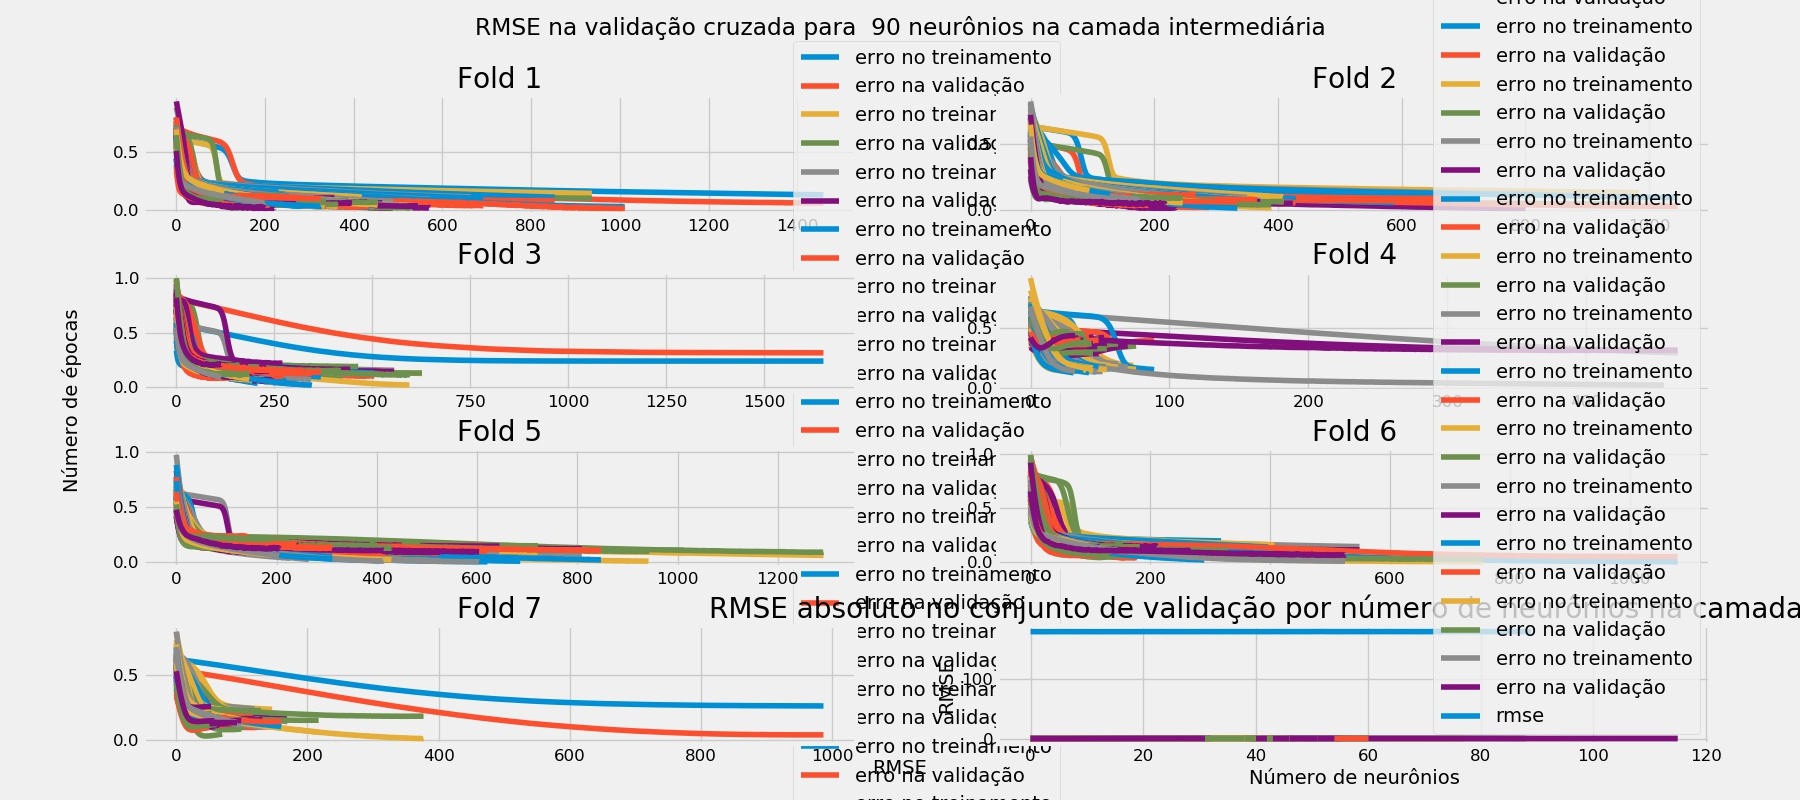
\includegraphics[width=\textwidth]{rmse_val_set_t3.jpg}
				
				\caption[\small{RMSE pelo n�mero de neur�nios no conjunto de valida��o para previs�o do PLD 3 meses � frente.}]{\label{rmseValT3} \small{RMSE pelo n�mero de neur�nios no conjunto de valida��o para previs�o do PLD 3 meses � frente.}}
				
			\end{center}
		}	
	\end{center}	
\end{figure}


\paragraph{}No conjunto de teste o resultado foi o seguinte:
\begin{figure}[H]
	\begin{center}
		{
			\begin{center}
				
				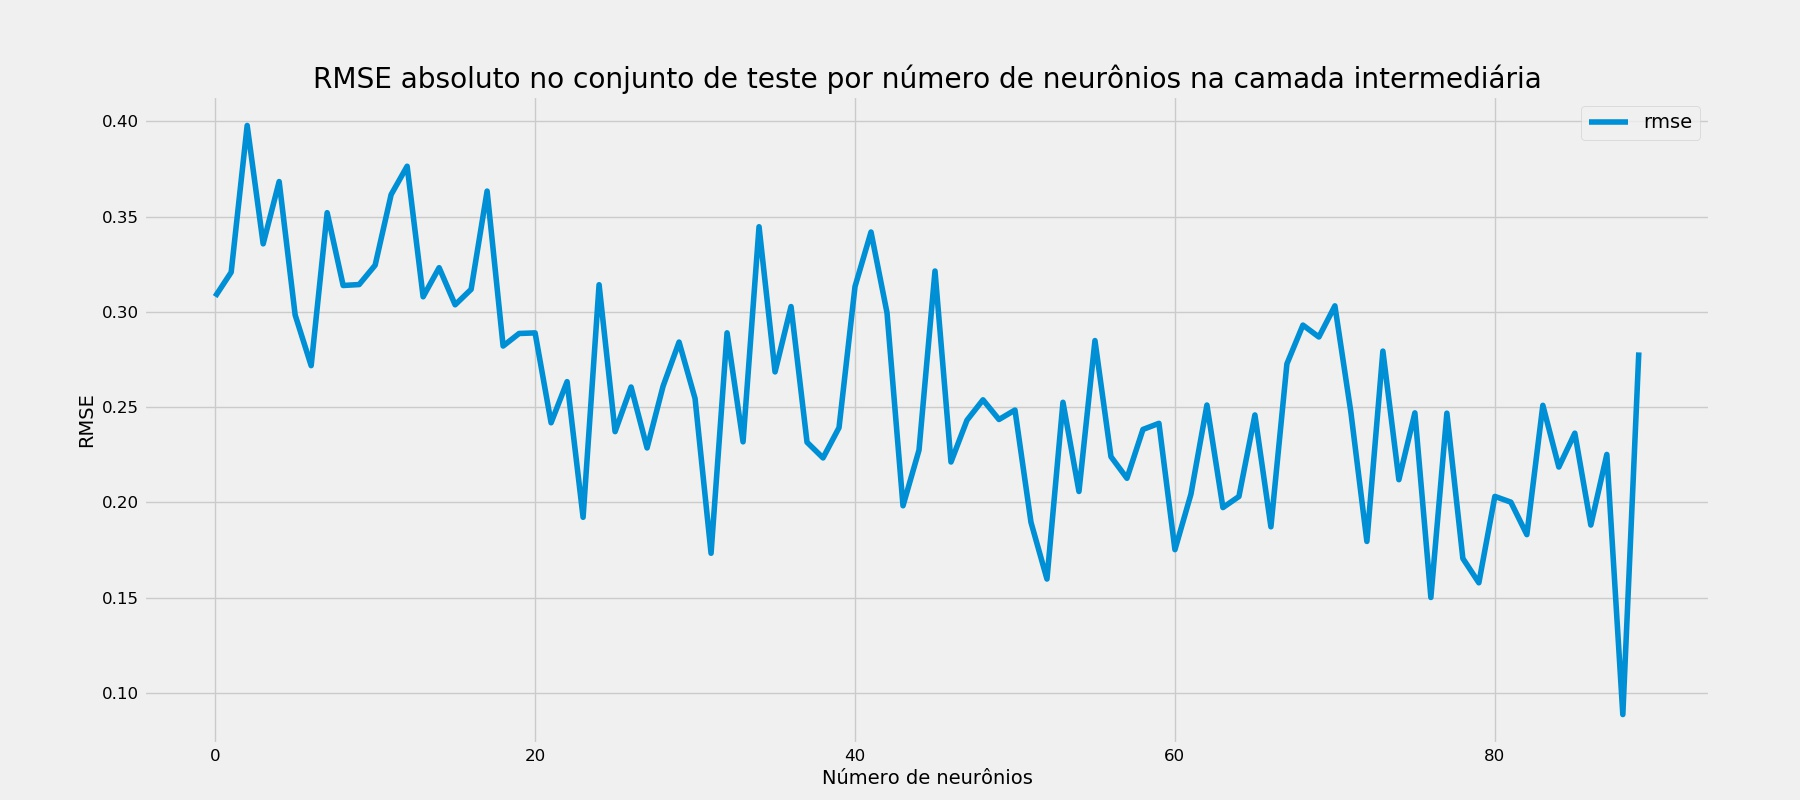
\includegraphics[width=\textwidth]{rmse_test_set_t3.jpg}
				
				\caption[\small{RMSE pelo n�mero de neur�nios no conjunto de teste para previs�o do PLD 3 meses � frente.}]{\label{rmseTestT3} \small{RMSE pelo n�mero de neur�nios no conjunto de teste para previs�o do PLD 3 meses � frente.}}
				
			\end{center}
		}	
	\end{center}	
\end{figure}


\begin{table}[H]	
	\begin{center}
		\caption{Resultados obtidos com as redes no dataset de valida��o para previs�o do PLD 3 meses � frente.}			
		\begin{tabular}{|c|c|c|c|c|c|c|c|}\hline \label{table:tabelaT3}
			
			\textbf{\#neur�nios} & \textbf{RMSE} & \textbf{STD} & \textbf{$a$ (m�dia)} & \textbf{$\epsilon_1$} & \textbf{$b$ (m�dia)} & \textbf{$\epsilon_2$} & \textbf{$\epsilon_3$}\\ \hline \vspace{-1.0mm}88 & 75,835 & 69,489 & 1,003 & 0,000 & 0,019 & 0,004 & 0,004  \\ \hline
			39 & 79,729 & 69,457 & 0,906 & 0,006 & -0,008 & 0,002 & 0,008  \\ \hline
			62 & 78,011 & 70,262 & 0,954 & 0,003 & 0,052 & 0,011 & 0,014  \\ \hline
			61 & 88,784 & 75,252 & 0,845 & 0,010 & 0,023 & 0,005 & 0,015  \\ \hline
			27 & 72,325 & 64,862 & 0,906 & 0,006 & 0,049 & 0,010 & 0,016  \\ \hline
		\end{tabular}
	\end{center}
\end{table}

\paragraph{}E com isso o modelo com 88 neur�nios foi escolhido. O treinamento dessa estrutura obteve os seguintes erros pelo n�mero de �pocas:

\begin{figure}[H]
	\begin{center}
		{
			\begin{center}
				
				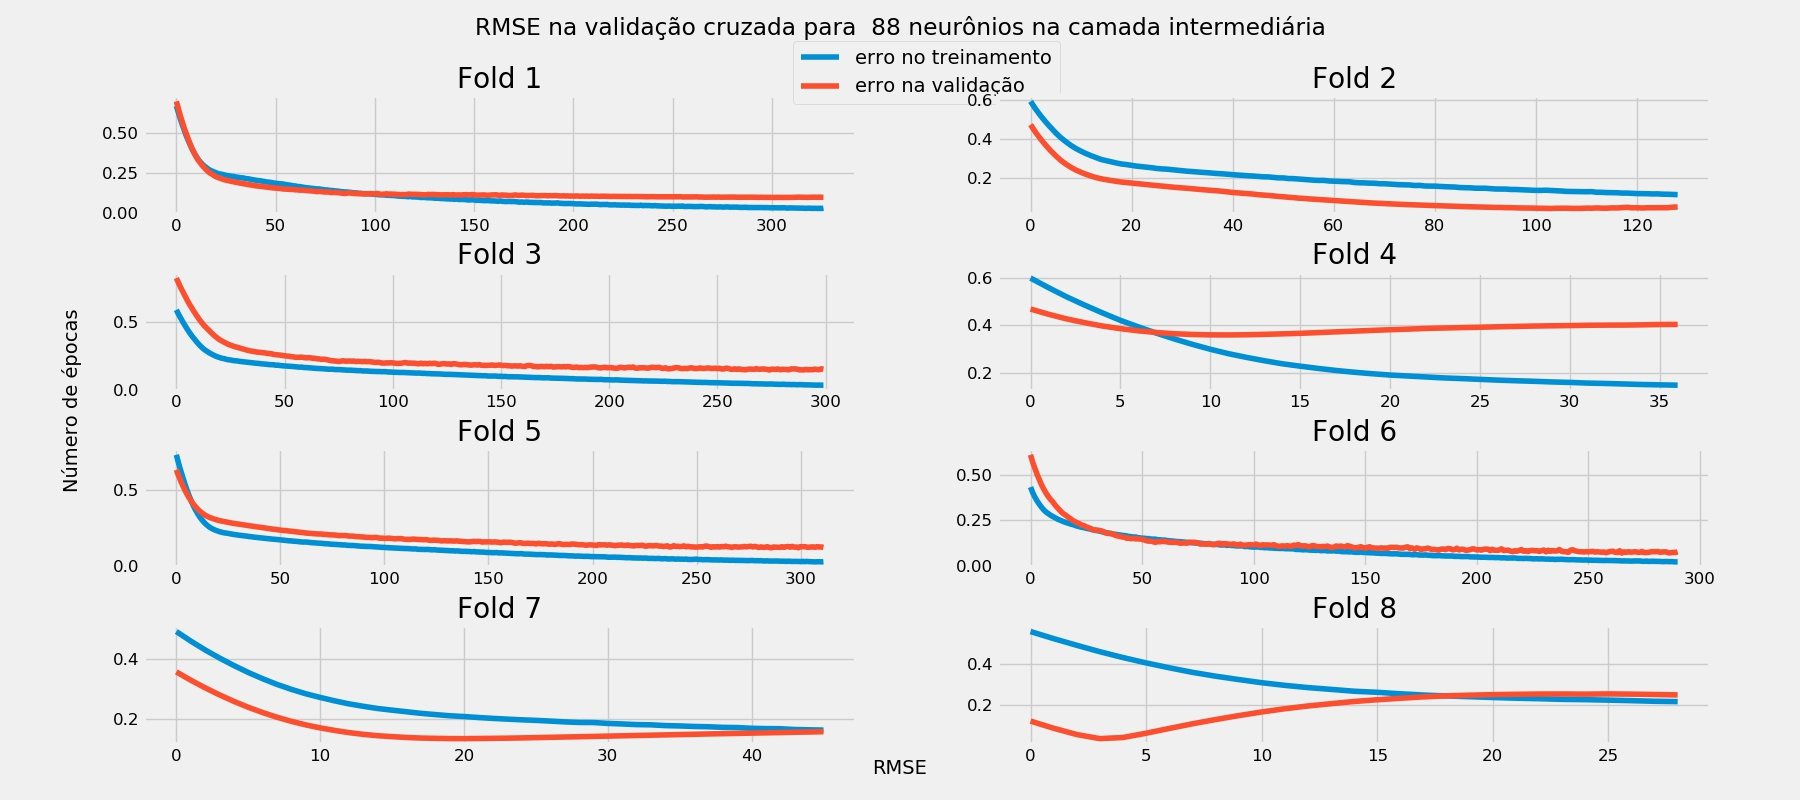
\includegraphics[width=\textwidth]{convergence_t3.jpg}
				
				\caption[\small{Erro pelo n�mero de �pocas e por subconjunto para previs�o do PLD 3 meses � frente.}]{\label{convT3} \small{Erro pelo n�mero de �pocas e por subconjunto para previs�o do PLD 3 meses � frente.}}
				
			\end{center}
		}	
	\end{center}	
\end{figure}

\paragraph{}E obteve-se os seguintes resultados:
\begin{figure}[H]
	\begin{center}
		{
			\begin{center}
				
				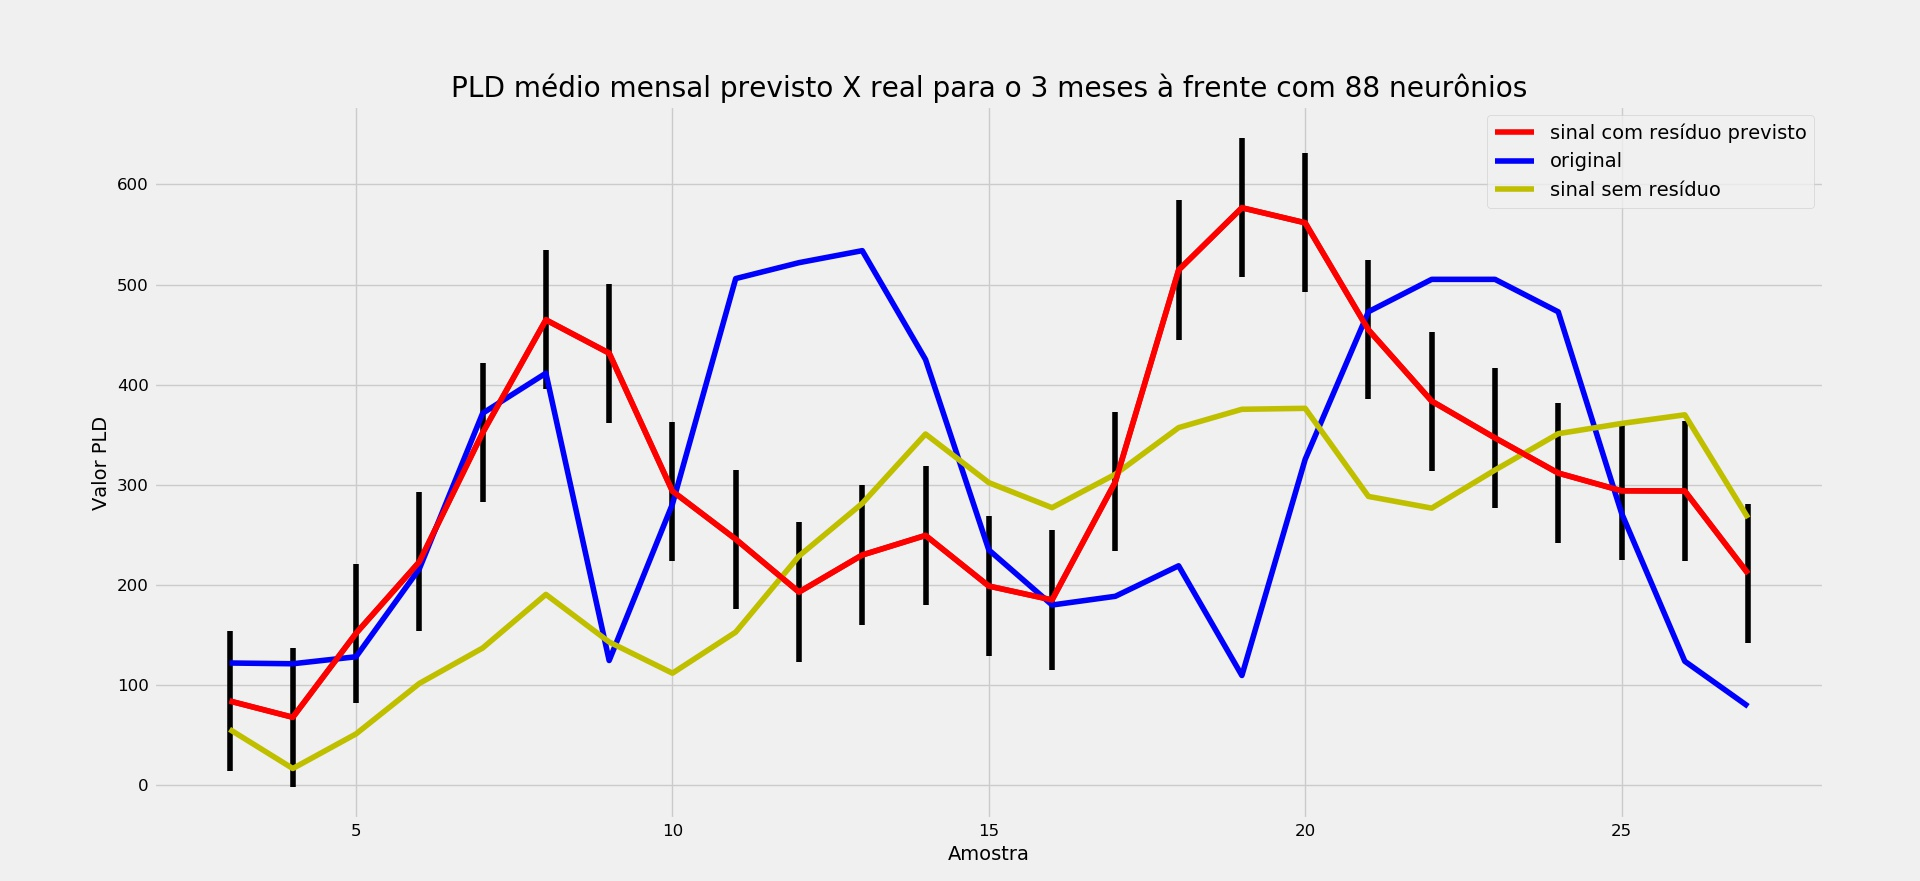
\includegraphics[width=\textwidth]{sinal_completo_t3.jpg}
				
				\caption[\small{Compara��o entre o sinal original e o resultado obtido para previs�o do PLD 3 meses � frente.}]{\label{completoT3} \small{Compara��o entre o sinal original e o resultado obtido para previs�o do PLD 3 meses � frente.}}
				
			\end{center}
		}	
	\end{center}	
\end{figure}

\section{Previs�o para 4 meses � frente}
\begin{figure}[H]
	\begin{center}
		{
			\begin{center}
				
				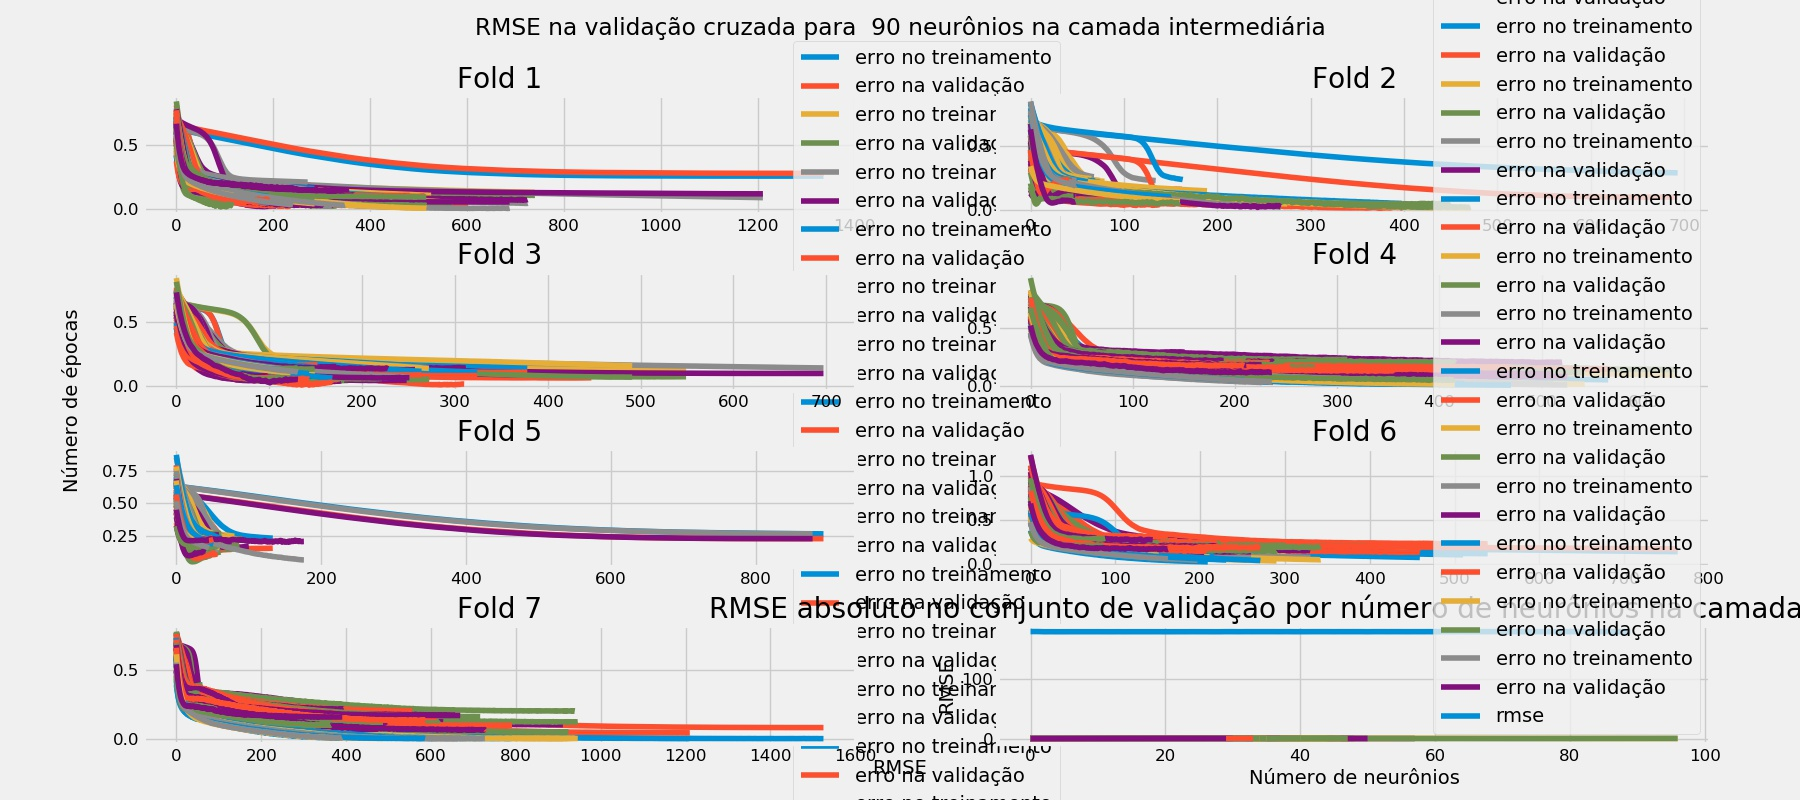
\includegraphics[width=\textwidth]{rmse_val_set_t4.jpg}
				
				\caption[\small{RMSE pelo n�mero de neur�nios no conjunto de valida��o para previs�o do PLD 4 meses � frente.}]{\label{rmseValT4} \small{RMSE pelo n�mero de neur�nios no conjunto de valida��o para previs�o do PLD 4 meses � frente.}}
				
			\end{center}
		}	
	\end{center}	
\end{figure}


\paragraph{}No conjunto de teste o resultado foi o seguinte:
\begin{figure}[H]
	\begin{center}
		{
			\begin{center}
				
				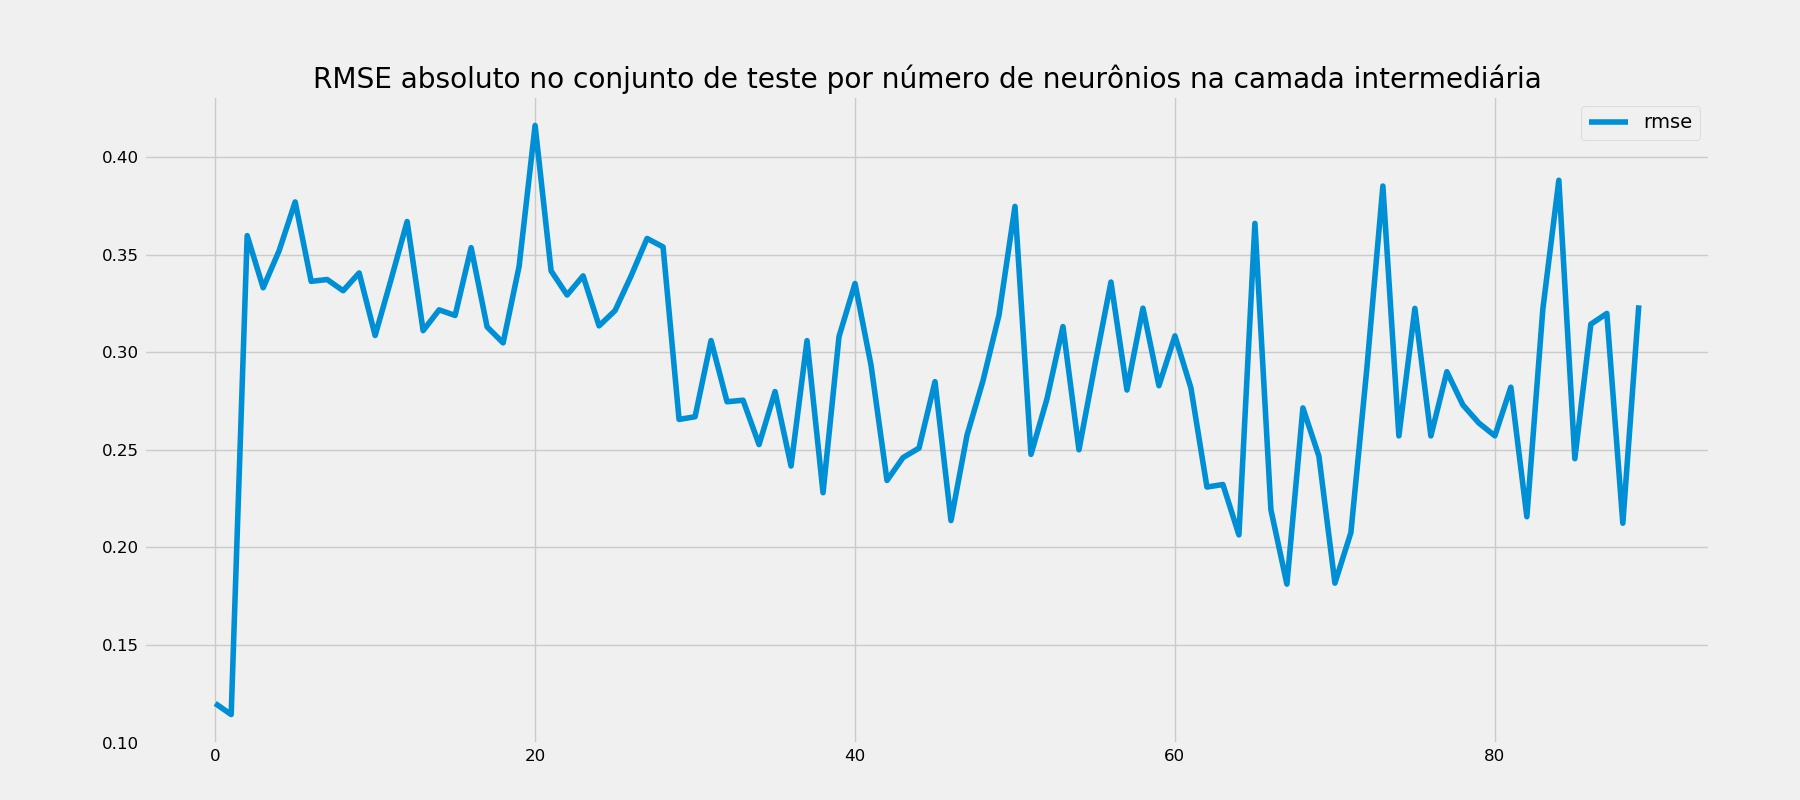
\includegraphics[width=\textwidth]{rmse_test_set_t4.jpg}
				
				\caption[\small{RMSE pelo n�mero de neur�nios no conjunto de teste para previs�o do PLD 4 meses � frente.}]{\label{rmseTestT4} \small{RMSE pelo n�mero de neur�nios no conjunto de teste para previs�o do PLD 4 meses � frente.}}
				
			\end{center}
		}	
	\end{center}	
\end{figure}


\begin{table}[H]	
	\begin{center}
		\caption{Resultados obtidos com as redes no dataset de valida��o para previs�o do PLD 4 meses � frente.}			
		\begin{tabular}{|c|c|c|c|c|c|c|c|}\hline \label{table:tabelaT4}
			
			\textbf{\#neur�nios} & \textbf{RMSE} & \textbf{STD} & \textbf{$a$ (m�dia)} & \textbf{$\epsilon_1$} & \textbf{$b$ (m�dia)} & \textbf{$\epsilon_2$} & \textbf{$\epsilon_3$}\\ \hline \vspace{-1.0mm}87 & 66,068 & 49,039 & 1,093 & 0,002 & 0,029 & 0,001 & 0,003 \\ \hline
			14 & 84,320 & 61,843 & 0,939 & 0,001 & 0,107 & 0,004 & 0,005 \\ \hline
			81 & 92,701 & 75,397 & 1,148 & 0,003 & 0,069 & 0,002 & 0,005 \\ \hline
			37 & 79,235 & 56,037 & 0,916 & 0,002 & 0,119 & 0,004 & 0,006 \\ \hline
			45 & 93,947 & 62,609 & 1,074 & 0,001 & 0,127 & 0,004 & 0,006 \\ \hline
		\end{tabular}	
	\end{center}
\end{table}

\paragraph{}E com isso o modelo com 88 neur�nios foi escolhido. O treinamento dessa estrutura obteve os seguintes erros pelo n�mero de �pocas:

\begin{figure}[H]
	\begin{center}
		{
			\begin{center}
				
				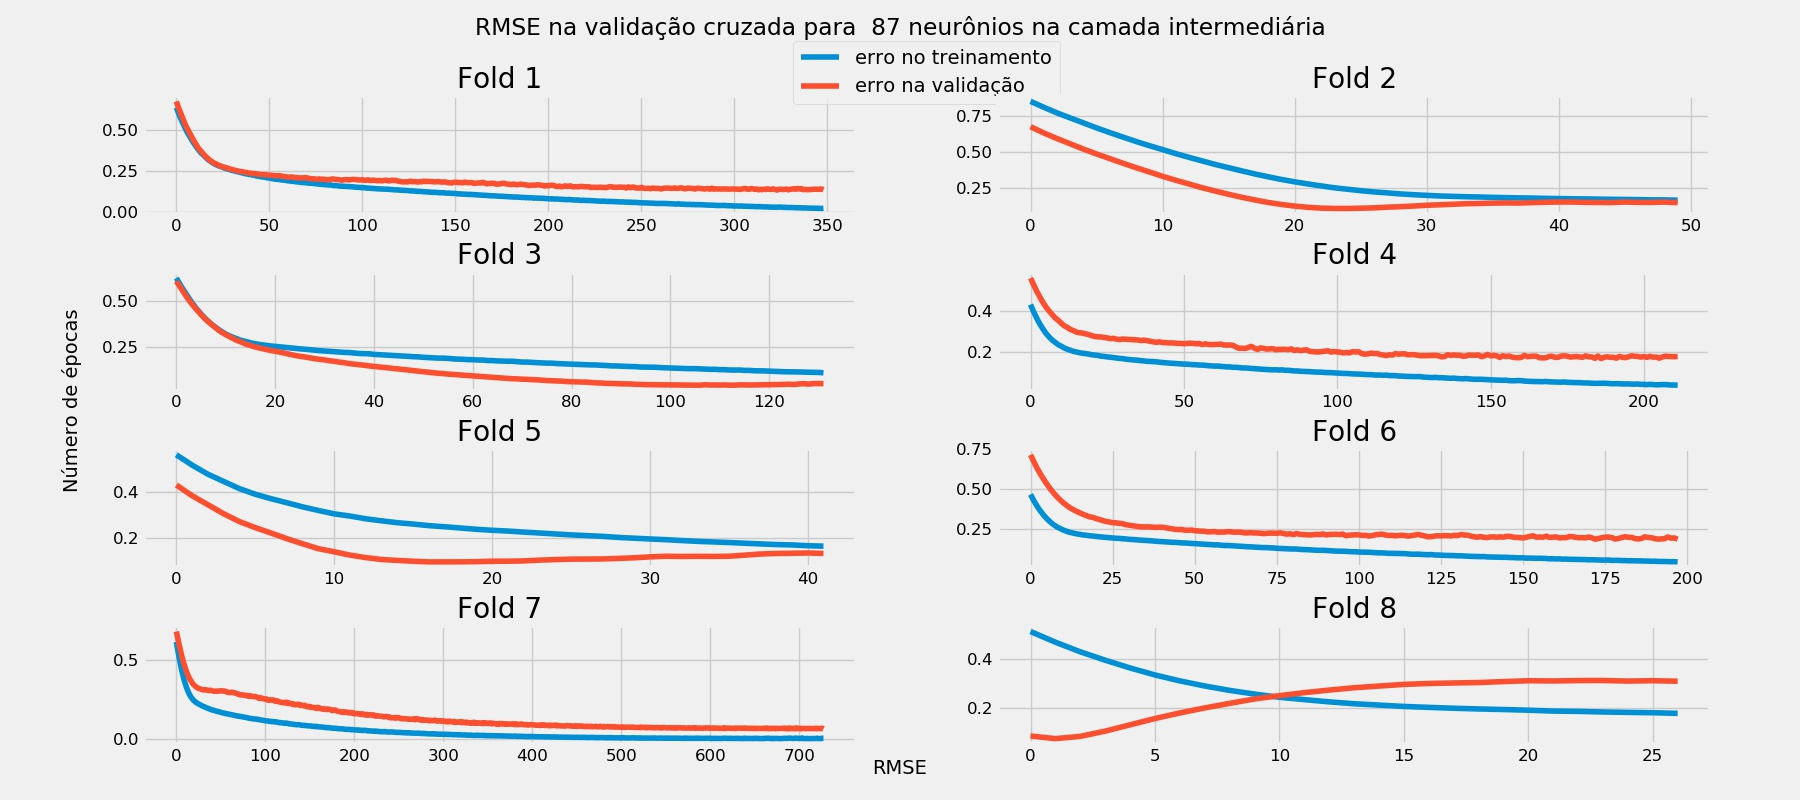
\includegraphics[width=\textwidth]{convergence_t4.jpg}
				
				\caption[\small{Erro pelo n�mero de �pocas e por subconjunto para previs�o do PLD 4 meses � frente.}]{\label{convT4} \small{Erro pelo n�mero de �pocas e por subconjunto para previs�o do PLD 4 meses � frente.}}
				
			\end{center}
		}	
	\end{center}	
\end{figure}

\paragraph{}E obteve-se os seguintes resultados:
\begin{figure}[H]
	\begin{center}
		{
			\begin{center}
				
				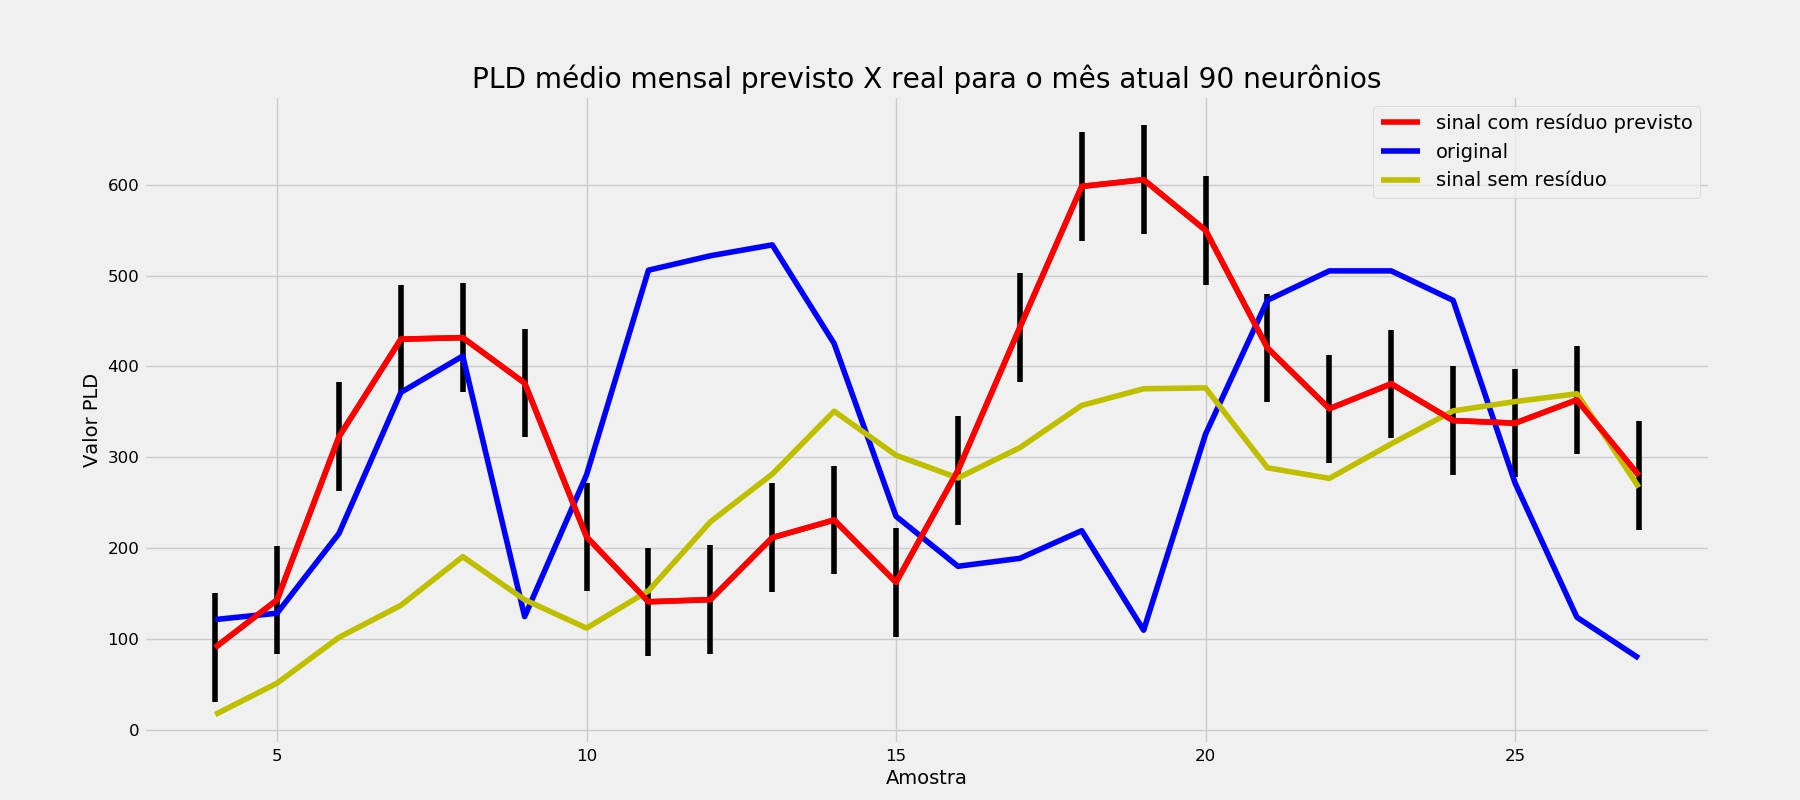
\includegraphics[width=\textwidth]{sinal_completo_t4.jpg}
				
				\caption[\small{Compara��o entre o sinal original e o resultado obtido para previs�o do PLD 4 meses � frente.}]{\label{completoT4} \small{Compara��o entre o sinal original e o resultado obtido para previs�o do PLD 4 meses � frente.}}
				
			\end{center}
		}	
	\end{center}	
\end{figure}

\section{Previs�o para 5 meses � frente}
\begin{figure}[H]
	\begin{center}
		{
			\begin{center}
				
				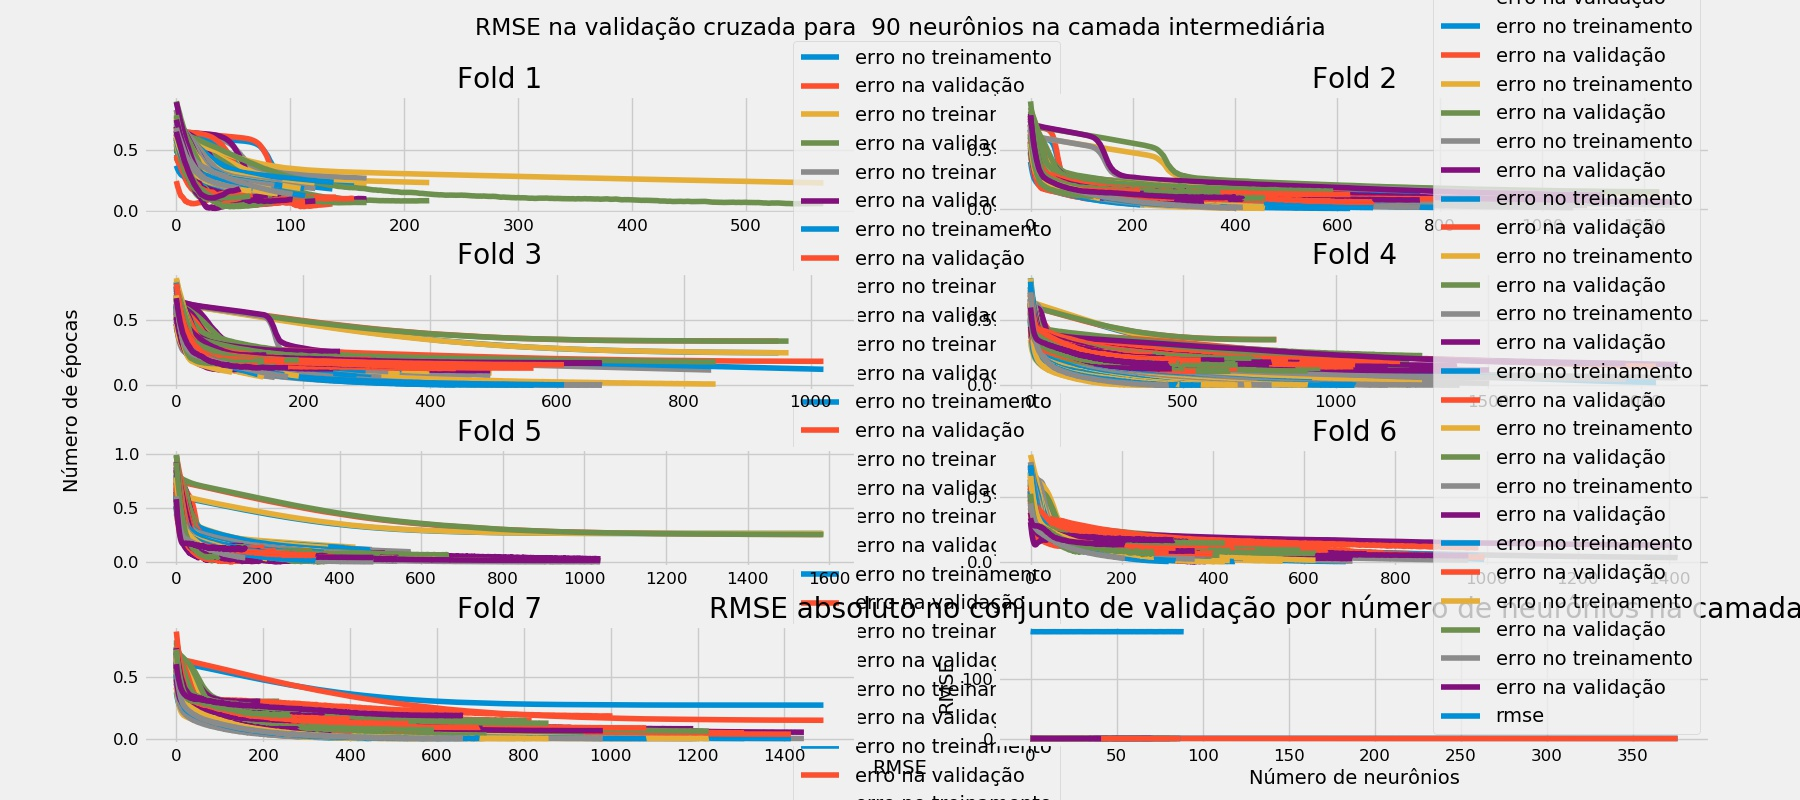
\includegraphics[width=\textwidth]{rmse_val_set_t5.jpg}
				
				\caption[\small{RMSE pelo n�mero de neur�nios no conjunto de valida��o para previs�o do PLD 5 meses � frente.}]{\label{rmseValT5} \small{RMSE pelo n�mero de neur�nios no conjunto de valida��o para previs�o do PLD 5 meses � frente.}}
				
			\end{center}
		}	
	\end{center}	
\end{figure}


\paragraph{}No conjunto de teste o resultado foi o seguinte:
\begin{figure}[H]
	\begin{center}
		{
			\begin{center}
				
				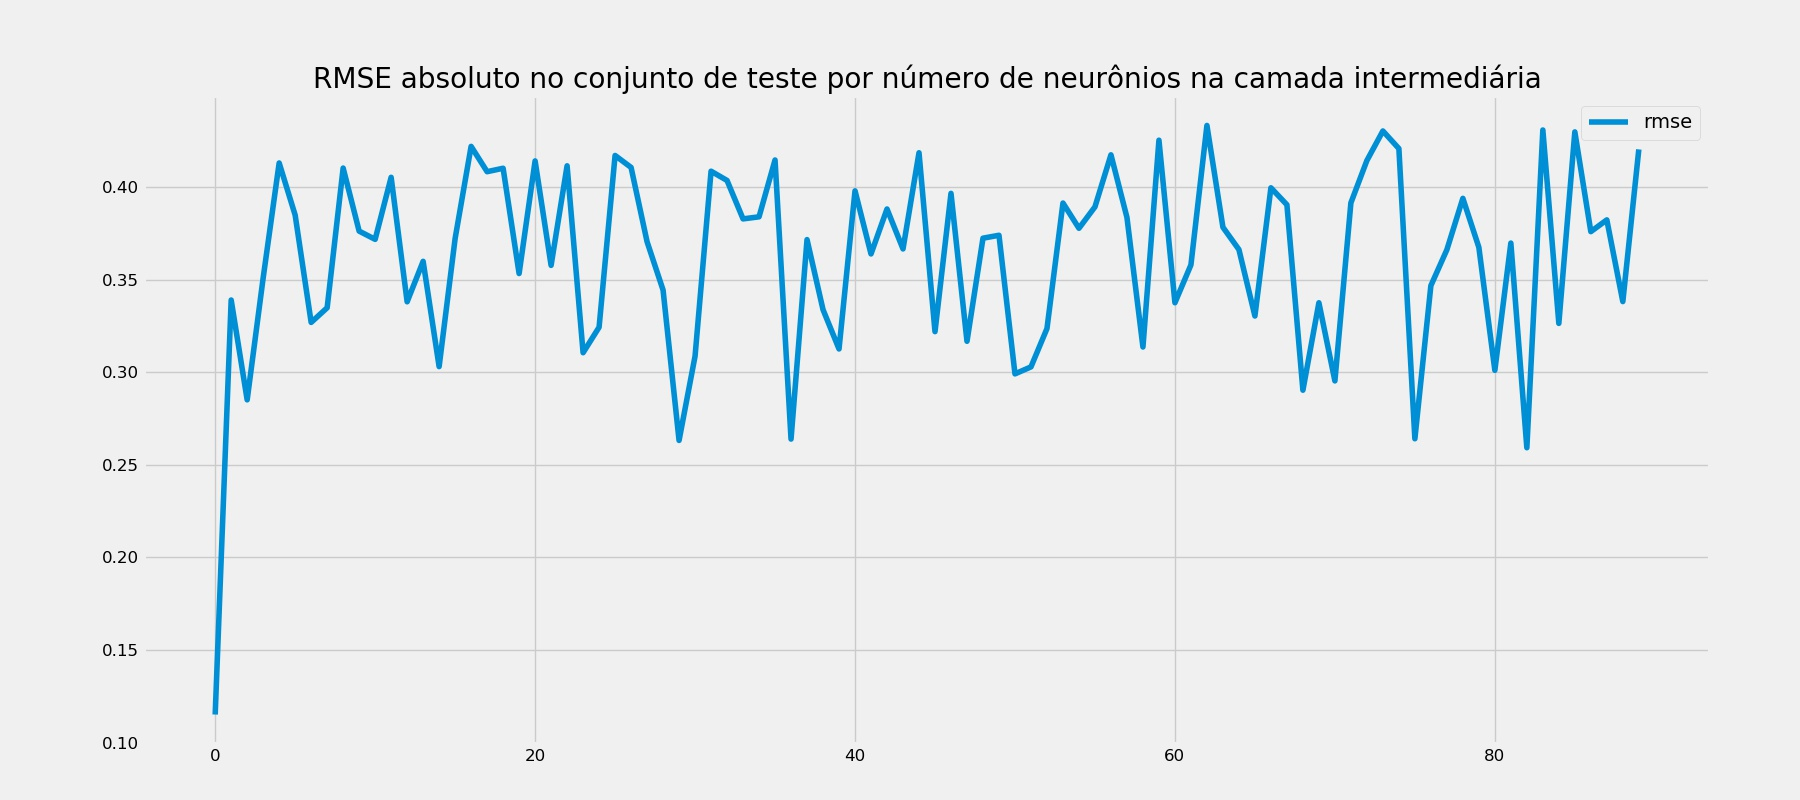
\includegraphics[width=\textwidth]{rmse_test_set_t5.jpg}
				
				\caption[\small{RMSE pelo n�mero de neur�nios no conjunto de teste para previs�o do PLD 5 meses � frente.}]{\label{rmseTestT5} \small{RMSE pelo n�mero de neur�nios no conjunto de teste para previs�o do PLD 5 meses � frente.}}
				
			\end{center}
		}	
	\end{center}	
\end{figure}


\begin{table}[H]	
	\begin{center}
		\caption{Resultados obtidos com as redes no dataset de valida��o para previs�o do PLD 5 meses � frente.}			
		\begin{tabular}{|c|c|c|c|c|c|c|c|}\hline \label{table:tabelaT5}
			
			\textbf{\#neur�nios} & \textbf{RMSE} & \textbf{STD} & \textbf{$a$ (m�dia)} & \textbf{$\epsilon_1$} & \textbf{$b$ (m�dia)} & \textbf{$\epsilon_2$} & \textbf{$\epsilon_3$}\\ \hline \vspace{-1.0mm}34 & 63,022 & 54,479 & 0,956 & 0,000 & -0,014 & 0,000 & 0,001 \\ \hline
			90 & 72,624 & 68,375 & 1,067 & 0,001 & -0,005 & 0,000 & 0,001 \\ \hline
			53 & 62,794 & 56,172 & 0,916 & 0,001 & -0,002 & 0,000 & 0,001 \\ \hline
			86 & 62,563 & 57,758 & 1,033 & 0,000 & -0,038 & 0,001 & 0,001 \\ \hline
			41 & 66,194 & 62,095 & 0,970 & 0,000 & -0,047 & 0,001 & 0,001 \\ \hline
			
		\end{tabular}
	\end{center}
\end{table}

\paragraph{}E com isso o modelo com 34 neur�nios foi escolhido. O treinamento dessa estrutura obteve os seguintes erros pelo n�mero de �pocas:

\begin{figure}[H]
	\begin{center}
		{
			\begin{center}
				
				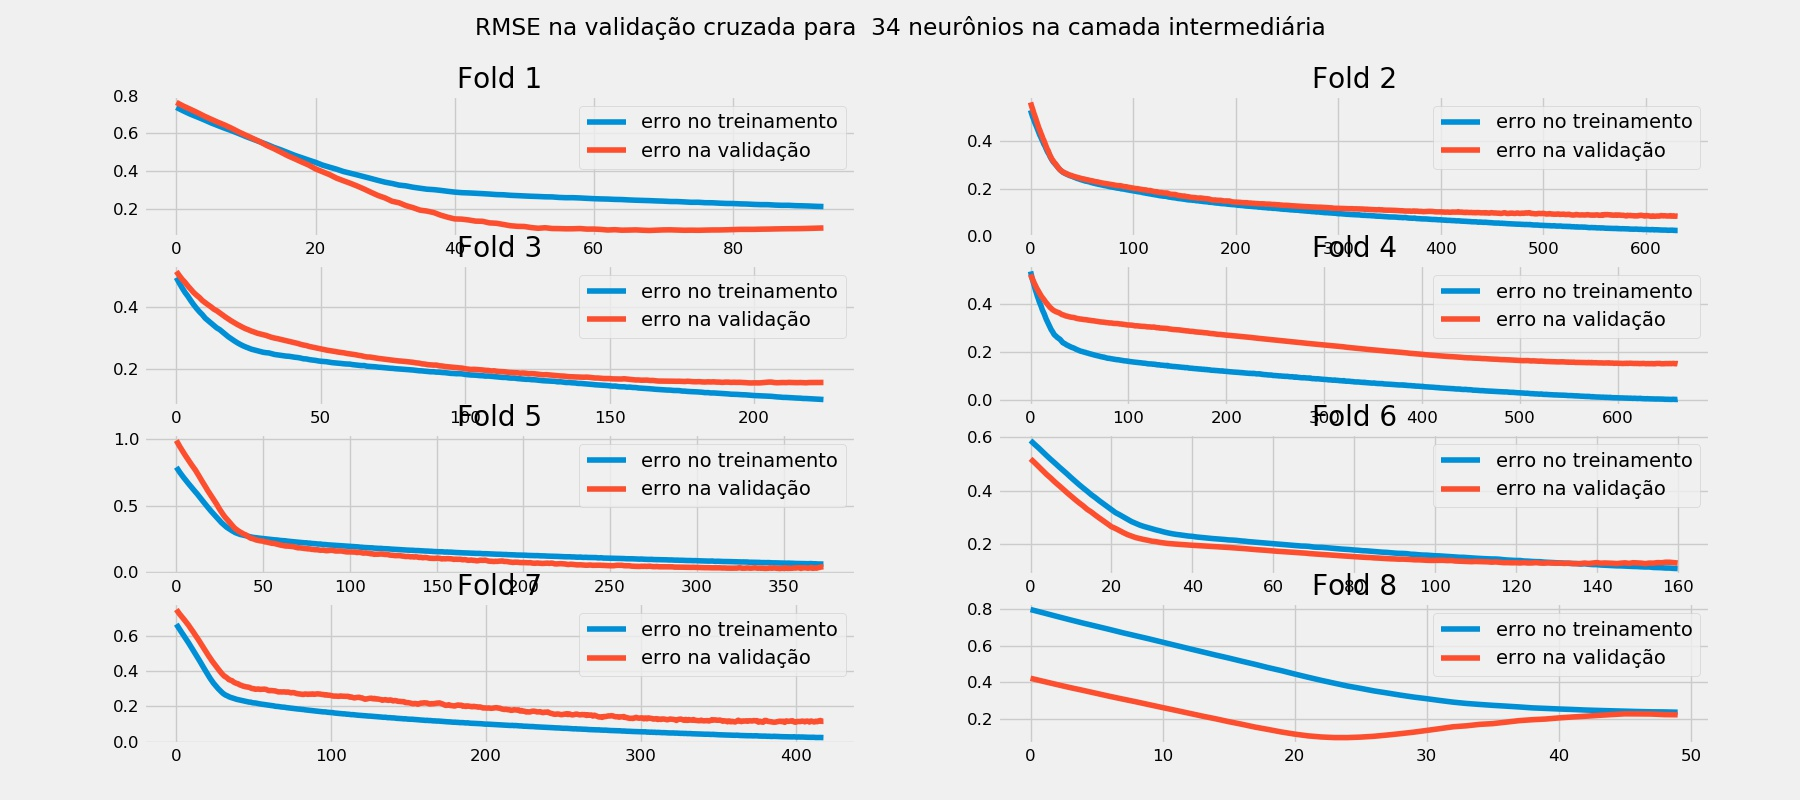
\includegraphics[width=\textwidth]{convergence_t5.jpg}
				
				\caption[\small{Erro pelo n�mero de �pocas e por subconjunto para previs�o do PLD 5 meses � frente.}]{\label{convT5} \small{Erro pelo n�mero de �pocas e por subconjunto para previs�o do PLD 5 meses � frente.}}
				
			\end{center}
		}	
	\end{center}	
\end{figure}

\paragraph{}E obteve-se os seguintes resultados:
\begin{figure}[H]
	\begin{center}
		{
			\begin{center}
				
				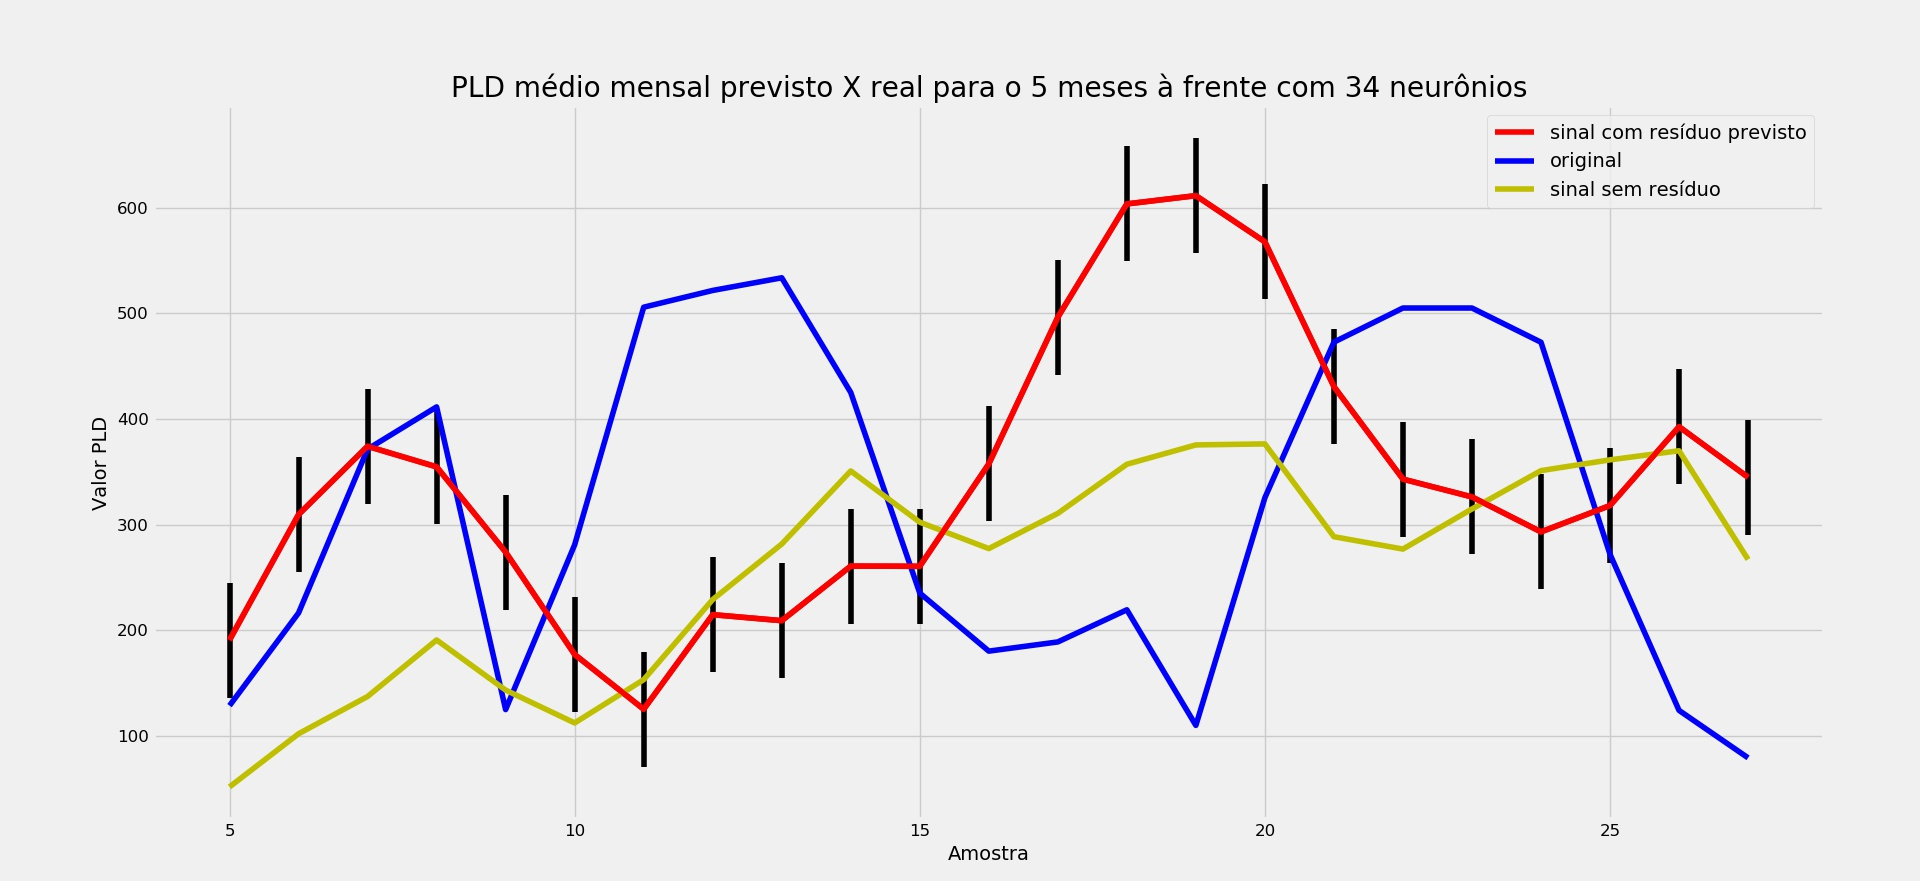
\includegraphics[width=\textwidth]{sinal_completo_t5.jpg}
				
				\caption[\small{Compara��o entre o sinal original e o resultado obtido para previs�o do PLD 5 meses � frente.}]{\label{completoT5} \small{Compara��o entre o sinal original e o resultado obtido para previs�o do PLD 5 meses � frente.}}
				
			\end{center}
		}	
	\end{center}	
\end{figure}

\section{Previs�o para 6 meses � frente}
\begin{figure}[H]
	\begin{center}
		{
			\begin{center}
				
				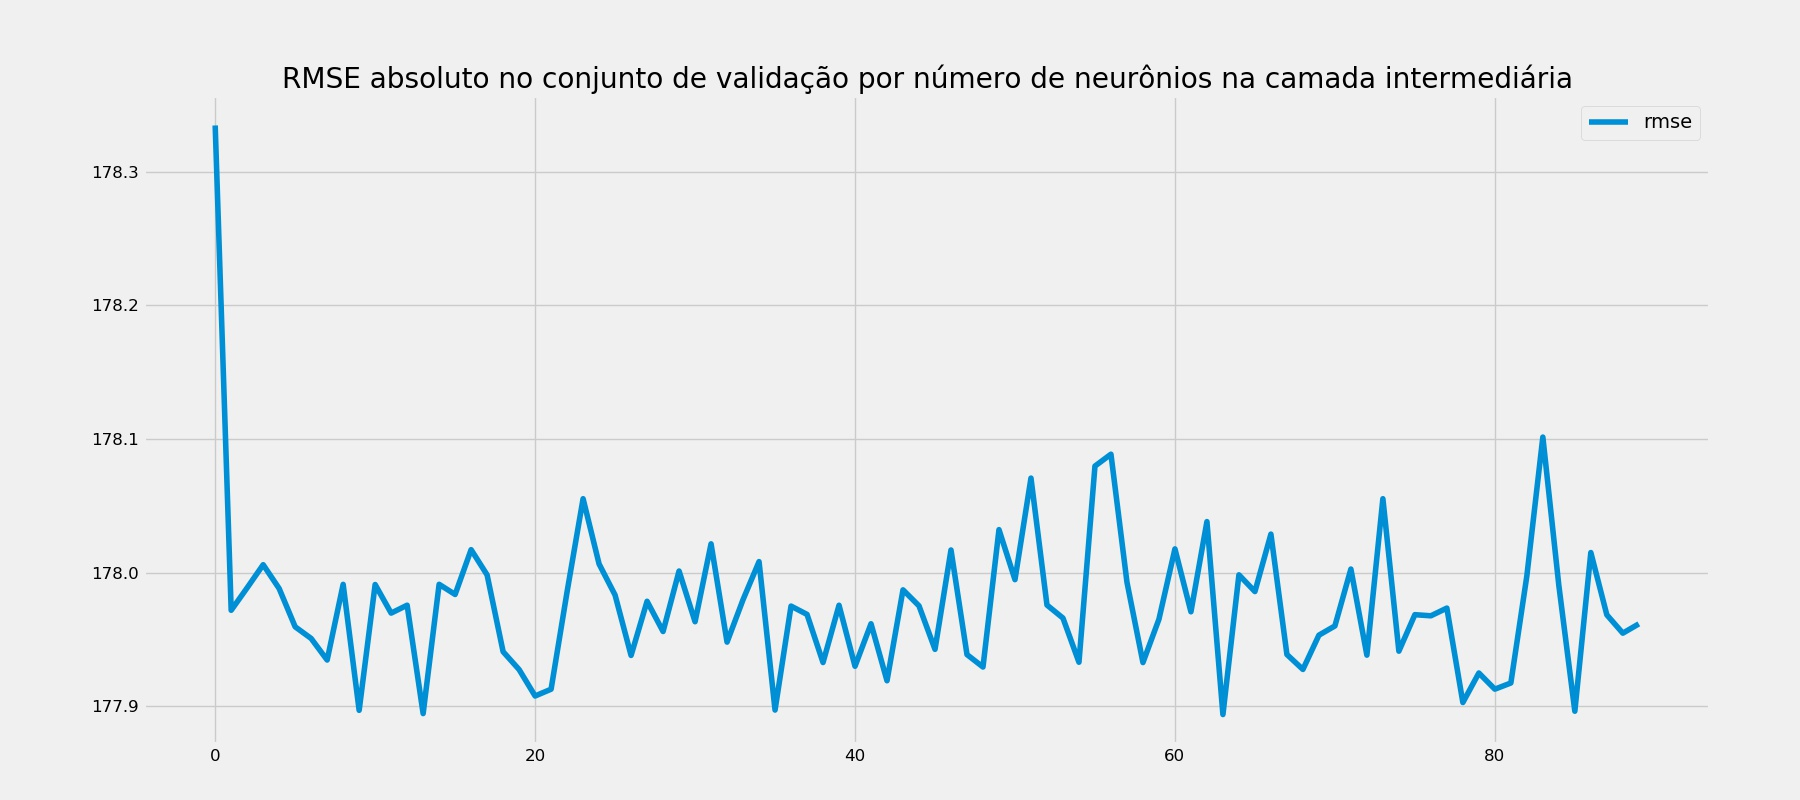
\includegraphics[width=\textwidth]{rmse_val_set_t6.jpg}
				
				\caption[\small{RMSE pelo n�mero de neur�nios no conjunto de valida��o para previs�o do PLD 6 meses � frente.}]{\label{rmseValT6} \small{RMSE pelo n�mero de neur�nios no conjunto de valida��o.}}
				
			\end{center}
		}	
	\end{center}	
\end{figure}


\paragraph{}No conjunto de teste o resultado foi o seguinte:
\begin{figure}[H]
	\begin{center}
		{
			\begin{center}
				
				\includegraphics[width=\textwidth]{rmse_test_set_t6.jpg}
				
				\caption[\small{RMSE pelo n�mero de neur�nios no conjunto de teste para previs�o do PLD 6 meses � frente.}]{\label{rmseTestT6} {RMSE pelo n�mero de neur�nios no conjunto de teste para previs�o do PLD 6 meses � frente.}}
				
			\end{center}
		}	
	\end{center}	
\end{figure}


\begin{table}[H]	
	\begin{center}
		\caption{Resultados obtidos com as redes no dataset de valida��o para previs�o do PLD 6 meses � frente.}			
		\begin{tabular}{|c|c|c|c|c|c|c|c|}\hline \label{table:tabelaT6}
			
			\textbf{\#neur�nios} & \textbf{RMSE} & \textbf{STD} & \textbf{$a$ (m�dia)} & \textbf{$\epsilon_1$} & \textbf{$b$ (m�dia)} & \textbf{$\epsilon_2$} & \textbf{$\epsilon_3$}\\ \hline \vspace{-1.0mm}57 & 88,770 & 79,111 & 0,975 & 0,000 & -0,008 & 0,000 & 0,001 \\ \hline
			20 & 95,084 & 88,687 & 0,953 & 0,001 & -0,007 & 0,000 & 0,001 \\ \hline
			71 & 81,320 & 75,164 & 1,074 & 0,001 & 0,001 & 0,000 & 0,001 \\ \hline
			85 & 73,433 & 70,922 & 0,978 & 0,000 & 0,032 & 0,001 & 0,002 \\ \hline
			17 & 72,576 & 66,944 & 1,089 & 0,002 & -0,028 & 0,001 & 0,003 \\ \hline
		\end{tabular}
	\end{center}
\end{table}

\paragraph{}E com isso o modelo com 57 neur�nios foi escolhido. O treinamento dessa estrutura obteve os seguintes erros pelo n�mero de �pocas:

\begin{figure}[H]
	\begin{center}
		{
			\begin{center}
				
				\includegraphics[width=\textwidth]{convergence_t6.jpg}
				
				\caption[\small{Erro pelo n�mero de �pocas e por subconjunto para previs�o do PLD 6 meses � frente.}]{\label{convT6} \small{Erro pelo n�mero de �pocas e por subconjunto para previs�o do PLD 6 meses � frente.}}
				
			\end{center}
		}	
	\end{center}	
\end{figure}

\paragraph{}E obteve-se os seguintes resultados:
\begin{figure}[H]
	\begin{center}
		{
			\begin{center}
				
				\includegraphics[width=\textwidth]{sinal_completo_t6.jpg}
				
				\caption[\small{Compara��o entre o sinal original e o resultado obtido para previs�o do PLD 6 meses � frente.}]{\label{completoT6} \small{Compara��o entre o sinal original e o resultado obtido para previs�o do PLD 6 meses � frente.}}
				
			\end{center}
		}	
	\end{center}	
\end{figure}

\section{Previs�o para 7 meses � frente}
\begin{figure}[H]
	\begin{center}
		{
			\begin{center}
				
				\includegraphics[width=\textwidth]{rmse_val_set_t7.jpg}
				
				\caption[\small{RMSE pelo n�mero de neur�nios no conjunto de valida��o para previs�o do PLD 7 meses � frente.}]{\label{rmseValT7} \small{RMSE pelo n�mero de neur�nios no conjunto de valida��o para previs�o do PLD 7 meses � frente.}}
				
			\end{center}
		}	
	\end{center}	
\end{figure}


\paragraph{}No conjunto de teste o resultado foi o seguinte:
\begin{figure}[H]
	\begin{center}
		{
			\begin{center}
				
				\includegraphics[width=\textwidth]{rmse_test_set_t7.jpg}
				
				\caption[\small{RMSE pelo n�mero de neur�nios no conjunto de teste.}]{\label{rmseTestT7} \small{RMSE pelo n�mero de neur�nios no conjunto de teste para previs�o do PLD 7 meses � frente.}}
				
			\end{center}
		}	
	\end{center}	
\end{figure}


\begin{table}[H]	
	\begin{center}
		\caption{Resultados obtidos com as redes no dataset de valida��o para previs�o do PLD 7 meses � frente.}			
		\begin{tabular}{|c|c|c|c|c|c|c|c|}\hline \label{table:tabelaT7}
			
			\textbf{\#neur�nios} & \textbf{RMSE} & \textbf{STD} & \textbf{$a$ (m�dia)} & \textbf{$\epsilon_1$} & \textbf{$b$ (m�dia)} & \textbf{$\epsilon_2$} & \textbf{$\epsilon_3$}\\ \hline \vspace{-1.0mm}85 & 81,374 & 74,638 & 1,073 & 0,001 & -0,015 & 0,000 & 0,001 \\ \hline
			59 & 87,220 & 79,156 & 0,963 & 0,000 & 0,034 & 0,001 & 0,001 \\ \hline
			55 & 94,054 & 84,463 & 0,964 & 0,000 & -0,041 & 0,001 & 0,001 \\ \hline
			88 & 88,838 & 80,536 & 1,105 & 0,001 & -0,038 & 0,001 & 0,002 \\ \hline
			45 & 82,782 & 78,053 & 0,891 & 0,001 & -0,048 & 0,001 & 0,002 \\ \hline
		\end{tabular}
	\end{center}
\end{table}

\paragraph{}E com isso o modelo com 85 neur�nios foi escolhido. O treinamento dessa estrutura obteve os seguintes erros pelo n�mero de �pocas:

\begin{figure}[H]
	\begin{center}
		{
			\begin{center}
				
				\includegraphics[width=\textwidth]{convergence_t7.jpg}
				
				\caption[\small{Erro pelo n�mero de �pocas e por subconjunto.}]{\label{convT7} \small{Erro pelo n�mero de �pocas e por subconjunto para previs�o do PLD 7 meses � frente.}}
				
			\end{center}
		}	
	\end{center}	
\end{figure}

\paragraph{}E obteve-se os seguintes resultados:
\begin{figure}[H]
	\begin{center}
		{
			\begin{center}
				
				\includegraphics[width=\textwidth]{sinal_completo_t7.jpg}
				
				\caption[\small{Compara��o entre o sinal original e o resultado obtido para previs�o do PLD 7 meses � frente.}]{\label{completoT7} \small{Compara��o entre o sinal original e o resultado obtido para previs�o do PLD 7 meses � frente.}}
				
			\end{center}
		}	
	\end{center}	
\end{figure}

\section{Previs�o para 8 meses � frente}
\begin{figure}[H]
	\begin{center}
		{
			\begin{center}
				
				\includegraphics[width=\textwidth]{rmse_val_set_t8.jpg}
				
				\caption[\small{RMSE pelo n�mero de neur�nios no conjunto de valida��o para previs�o do PLD 7 meses � frente.}]{\label{rmseValT8} \small{RMSE pelo n�mero de neur�nios no conjunto de valida��o para previs�o do PLD 7 meses � frente.}}
				
			\end{center}
		}	
	\end{center}	
\end{figure}


\paragraph{}No conjunto de teste o resultado foi o seguinte:
\begin{figure}[H]
	\begin{center}
		{
			\begin{center}
				
				\includegraphics[width=\textwidth]{rmse_test_set_t8.jpg}
				
				\caption[\small{RMSE pelo n�mero de neur�nios no conjunto de teste para previs�o do PLD 8 meses � frente.}]{\label{rmseTestT8} \small{RMSE pelo n�mero de neur�nios no conjunto de teste para previs�o do PLD 8 meses � frente.}}
				
			\end{center}
		}	
	\end{center}	
\end{figure}


\begin{table}[H]	
	\begin{center}
		\caption{Resultados obtidos com as redes no dataset de valida��o para previs�o do PLD 8 meses � frente.}			
		\begin{tabular}{|c|c|c|c|c|c|c|c|}\hline \label{table:tabelaT8}
			
			\textbf{\#neur�nios} & \textbf{RMSE} & \textbf{STD} & \textbf{$a$ (m�dia)} & \textbf{$\epsilon_1$} & \textbf{$b$ (m�dia)} & \textbf{$\epsilon_2$} & \textbf{$\epsilon_3$}\\ \hline \vspace{-1.0mm}29 & 93,498 & 61,547 & 1,060 & 0,001 & -0,002 & 0,000 & 0,001 \\ \hline
			24 & 94,052 & 69,505 & 1,055 & 0,001 & -0,035 & 0,001 & 0,002 \\ \hline
			9 & 83,198 & 57,893 & 1,089 & 0,001 & -0,029 & 0,001 & 0,002 \\ \hline
			66 & 86,705 & 61,198 & 1,068 & 0,001 & -0,042 & 0,001 & 0,002 \\ \hline
			51 & 92,674 & 62,083 & 1,036 & 0,001 & 0,060 & 0,002 & 0,003 \\ \hline
		\end{tabular}
	\end{center}
\end{table}

\paragraph{}E com isso o modelo com 29 neur�nios foi escolhido. O treinamento dessa estrutura obteve os seguintes erros pelo n�mero de �pocas:

\begin{figure}[H]
	\begin{center}
		{
			\begin{center}
				
				\includegraphics[width=\textwidth]{convergence_t8.jpg}
				
				\caption[\small{Erro pelo n�mero de �pocas e por subconjunto para previs�o do PLD 8 meses � frente.}]{\label{convT8} \small{Erro pelo n�mero de �pocas e por subconjunto para previs�o do PLD 8 meses � frente.}}
				
			\end{center}
		}	
	\end{center}	
\end{figure}

\paragraph{}E obteve-se os seguintes resultados:
\begin{figure}[H]
	\begin{center}
		{
			\begin{center}
				
				\includegraphics[width=\textwidth]{sinal_completo_t8.jpg}
				
				\caption[\small{Compara��o entre o sinal original e o resultado obtido para previs�o do PLD 8 meses � frente.}]{\label{completoT8} \small{Compara��o entre o sinal original e o resultado obtido para previs�o do PLD 8 meses � frente.}}
				
			\end{center}
		}	
	\end{center}	
\end{figure}

\section{Previs�o para 9 meses � frente}
\begin{figure}[H]
	\begin{center}
		{
			\begin{center}
				
				\includegraphics[width=\textwidth]{rmse_val_set_t9.jpg}
				
				\caption[\small{RMSE pelo n�mero de neur�nios no conjunto de valida��o para previs�o do PLD 9 meses � frente.}]{\label{rmseValT9} \small{RMSE pelo n�mero de neur�nios no conjunto de valida��o para previs�o do PLD 9 meses � frente.}}
				
			\end{center}
		}	
	\end{center}	
\end{figure}


\paragraph{}No conjunto de teste o resultado foi o seguinte:
\begin{figure}[H]
	\begin{center}
		{
			\begin{center}
				
				\includegraphics[width=\textwidth]{rmse_test_set_t9.jpg}
				
				\caption[\small{RMSE pelo n�mero de neur�nios no conjunto de teste para previs�o do PLD 9 meses � frente.}]{\label{rmseTestT9} \small{RMSE pelo n�mero de neur�nios no conjunto de teste para previs�o do PLD 9 meses � frente.}}
				
			\end{center}
		}	
	\end{center}	
\end{figure}


\begin{table}[H]	
	\begin{center}
		\caption{Resultados obtidos com as redes no dataset de valida��o para previs�o do PLD 9 meses � frente.}			
		\begin{tabular}{|c|c|c|c|c|c|c|c|}\hline \label{table:tabelaT9}
			
			\textbf{\#neur�nios} & \textbf{RMSE} & \textbf{STD} & \textbf{$a$ (m�dia)} & \textbf{$\epsilon_1$} & \textbf{$b$ (m�dia)} & \textbf{$\epsilon_2$} & \textbf{$\epsilon_3$}\\ \hline \vspace{-1.0mm}66 & 53,146 & 35,811 & 0,968 & 0,000 & -0,132 & 0,001 & 0,002 \\ \hline
			30 & 81,717 & 66,631 & 1,147 & 0,001 & 0,050 & 0,000 & 0,002 \\ \hline
			39 & 74,664 & 53,134 & 0,996 & 0,000 & -0,220 & 0,002 & 0,002 \\ \hline
			74 & 63,687 & 45,221 & 0,708 & 0,002 & -0,017 & 0,000 & 0,002 \\ \hline
			90 & 93,000 & 79,354 & 0,944 & 0,000 & 0,220 & 0,002 & 0,003 \\ \hline
		\end{tabular}
	\end{center}
\end{table}

\paragraph{}E com isso o modelo com 66 neur�nios foi escolhido. O treinamento dessa estrutura obteve os seguintes erros pelo n�mero de �pocas:

\begin{figure}[H]
	\begin{center}
		{
			\begin{center}
				
				\includegraphics[width=\textwidth]{convergence_t9.jpg}
				
				\caption[\small{Erro pelo n�mero de �pocas e por subconjunto para previs�o do PLD 9 meses � frente.}]{\label{convT9} \small{Erro pelo n�mero de �pocas e por subconjunto para previs�o do PLD 9 meses � frente.}}
				
			\end{center}
		}	
	\end{center}	
\end{figure}

\paragraph{}E obteve-se os seguintes resultados:
\begin{figure}[H]
	\begin{center}
		{
			\begin{center}
				
				\includegraphics[width=\textwidth]{sinal_completo_t9.jpg}
				
				\caption[\small{Compara��o entre o sinal original e o resultado obtido para previs�o do PLD 9 meses � frente.}]{\label{completoT9} \small{Compara��o entre o sinal original e o resultado obtido para previs�o do PLD 9 meses � frente.}}
				
			\end{center}
		}	
	\end{center}	
\end{figure}

\section{Previs�o para 10 meses � frente}
\begin{figure}[H]
	\begin{center}
		{
			\begin{center}
				
				\includegraphics[width=\textwidth]{rmse_val_set_t10.jpg}
				
				\caption[\small{RMSE pelo n�mero de neur�nios no conjunto de valida��o para previs�o do PLD 10 meses � frente.}]{\label{rmseValT10} \small{RMSE pelo n�mero de neur�nios no conjunto de valida��o para previs�o do PLD 10 meses � frente.}}
				
			\end{center}
		}	
	\end{center}	
\end{figure}


\paragraph{}No conjunto de teste o resultado foi o seguinte:
\begin{figure}[H]
	\begin{center}
		{
			\begin{center}
				
				\includegraphics[width=\textwidth]{rmse_test_set_t10.jpg}
				
				\caption[\small{RMSE pelo n�mero de neur�nios no conjunto de teste.}]{\label{rmseTestT10} \small{RMSE pelo n�mero de neur�nios no conjunto de teste para previs�o do PLD 10 meses � frente.}}
				
			\end{center}
		}	
	\end{center}	
\end{figure}


\begin{table}[H]	
	\begin{center}
		\caption{Resultados obtidos com as redes no dataset de valida��o para previs�o do PLD 10 meses � frente.}			
		\begin{tabular}{|c|c|c|c|c|c|c|c|}\hline \label{table:tabelaT10}
			
			\textbf{\#neur�nios} & \textbf{RMSE} & \textbf{STD} & \textbf{$a$ (m�dia)} & \textbf{$\epsilon_1$} & \textbf{$b$ (m�dia)} & \textbf{$\epsilon_2$} & \textbf{$\epsilon_3$}\\ \hline \vspace{-1.0mm}74 & 47,276 & 24,496 & 0,979 & 0,000 & 0,092 & 0,002 & 0,002 \\ \hline
			82 & 50,150 & 38,221 & 0,794 & 0,002 & -0,065 & 0,002 & 0,004 \\ \hline
			86 & 71,629 & 49,838 & 0,744 & 0,003 & -0,061 & 0,001 & 0,004 \\ \hline
			55 & 47,440 & 34,009 & 1,408 & 0,005 & 0,011 & 0,000 & 0,005 \\ \hline
			32 & 41,108 & 27,709 & 1,073 & 0,001 & 0,181 & 0,004 & 0,005 \\ \hline
		\end{tabular}
	\end{center}
\end{table}

\paragraph{}E com isso o modelo com 74 neur�nios foi escolhido. O treinamento dessa estrutura obteve os seguintes erros pelo n�mero de �pocas:

\begin{figure}[H]
	\begin{center}
		{
			\begin{center}
				
				\includegraphics[width=\textwidth]{convergence_t10.jpg}
				
				\caption[\small{Erro pelo n�mero de �pocas e por subconjunto para previs�o do PLD 10 meses � frente.}]{\label{convT10} \small{Erro pelo n�mero de �pocas e por subconjunto para previs�o do PLD 10 meses � frente.}}
				
			\end{center}
		}	
	\end{center}	
\end{figure}

\paragraph{}E obteve-se os seguintes resultados:
\begin{figure}[H]
	\begin{center}
		{
			\begin{center}
				
				\includegraphics[width=\textwidth]{sinal_completo_t10.jpg}
				
				\caption[\small{Compara��o entre o sinal original e o resultado obtido para previs�o do PLD 10 meses � frente.}]{\label{completoT10} \small{Compara��o entre o sinal original e o resultado obtido para previs�o do PLD 10 meses � frente.}}
				
			\end{center}
		}	
	\end{center}	
\end{figure}
   % ---------------------------------------------------------------
   % Ap�ndice B
   % ---------------------------------------------------------------
   \chapter{Encaderna��o do Projeto de Gradua��o}
   \label{ApendiceB}
   \begin{figure}
\begin{center}
\parbox[htb]{13.0cm}
  {
  \begin{center}
  \includegraphics[scale=1.0]{Capa_do_Projeto_Final.eps}
  \caption[\small{Encaderna��o do projeto de gradua��o.}]{\label{FigPFC} \small{Encaderna��o do projeto de gradua��o.}}
  \end{center}
  }
\end{center}
\end{figure}
   % ---------------------------------------------------------------
   % Ap�ndice C
   % ---------------------------------------------------------------
   \chapter{O que � um anexo}
   \label{ApendiceC}
   \paragraph{}Documenta��o n�o elaborada pelo autor, ou elaborada pelo autor mas constituindo parte de outro projeto.   

\backmatter

\end{document}
